%-------------------------------------------------------------------------------
%                                PREAMBLE
%-------------------------------------------------------------------------------
\documentclass[usenames,dvipsnames,svgnames,10pt,aspectratio=169]{beamer}
\usefonttheme{professionalfonts}

% This theme uses TIKZ: compile twice with PDFLaTeX or LuaLaTeX.
%
%  Options:
%  - [clean]:    clean slides, i.e. logos and footbar are removed
%  - [kth]:      footbar style inspierd to the official KTH template
%  - [nicewave]: a different style of wave is used (not approved by FLOW)
%
\usetheme{flow}

\usepackage{hyperref,graphicx,lmodern}
\usepackage[utf8]{inputenc}
\usepackage{media9}
\usepackage{xcolor}
\usepackage{stmaryrd}
\usepackage{nicefrac}
\usepackage{multimedia}
\usepackage{multicol}
\usepackage{upgreek}
\usepackage[]{bm}
\usepackage[]{url}

\DeclareMathOperator{\sinc}{sinc}
\DeclareMathAlphabet{\mathcal}{OMS}{cmsy}{m}{n}
\DeclareMathAlphabet\mathbfcal{OMS}{cmsy}{b}{n}
\DeclareMathOperator*{\minimize}{minimize~}
\DeclareMathOperator*{\subjectto}{subject~to~}

\graphicspath{{imgs/}}
\setbeamertemplate{blocks}[rounded][shadow=true]

\DeclareMathOperator{\trace}{tr}

%-------------------------------------------------------------------------------
%                                TITLE PAGE
%-------------------------------------------------------------------------------
\title[Nonlinear Physics] % Short title used in footline
{
	Nonlinear physics, dynamical \\ systems and chaos theory
}

\author[J.-Ch.~Loiseau] % Presenting author in short form used in footline
{
	Jean-Christophe Loiseau
}
% - Give the names in the same order as the appear in the paper.
% - Underline the presenting author.

\institute[unused]
{
	\url{jean-christophe.loiseau@ensam.eu} \\
	DynFluid, \\
	Arts et M\'etiers ParisTech, France
}
% Keep it simple, no one is interested in your street address.

% University logo(s)
\logot{
\includegraphics[width=.128\paperwidth]{DynFluid_logo}}  % Top logo
\logob{
\includegraphics[width=0.128\paperwidth]{ENSAM_logo}} % Bottom logo
% \logoc[{
\includegraphics[width=.128\paperwidth]{limsi}}]{
\includegraphics[width=.128\paperwidth]{limsi}} % Corner logo
%
% Cover image: \cvrimg{x position}{y position}{cover image}
\cvrimg{.77}{.8}{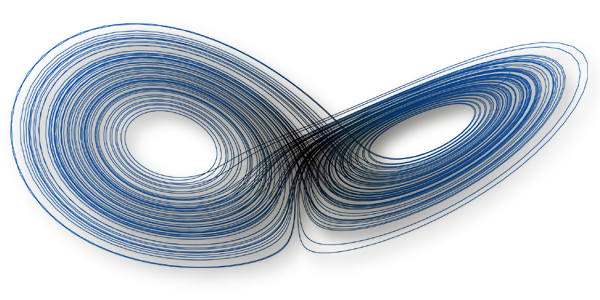
\includegraphics[width=.4\paperwidth]{cover.png}}

\date[unused]{ENSAM, Master 2, 2018--2019}

\begin{document}

\titleframe % Print the title as the first slide

%-------------------------------------------------------------------------------
%                           PRESENTATION SLIDES
%-------------------------------------------------------------------------------

\begin{frame}[t, c]{Today's menu}{Fractal geometry, chaos and strange attractors}
	\centering

	\begin{minipage}{.48\textwidth}
		\begin{itemize}
			\item Fractal geometry is the \emph{geometry of nature}.
			\medskip
			\item It is closely connected to chaotic dynamical systems.
			\medskip
			\item Formalized by B.\ Mandelbrot during the late 70's.
		\end{itemize}
	\end{minipage}%
	\hfill
	\begin{minipage}{.48\textwidth}
		\centering
		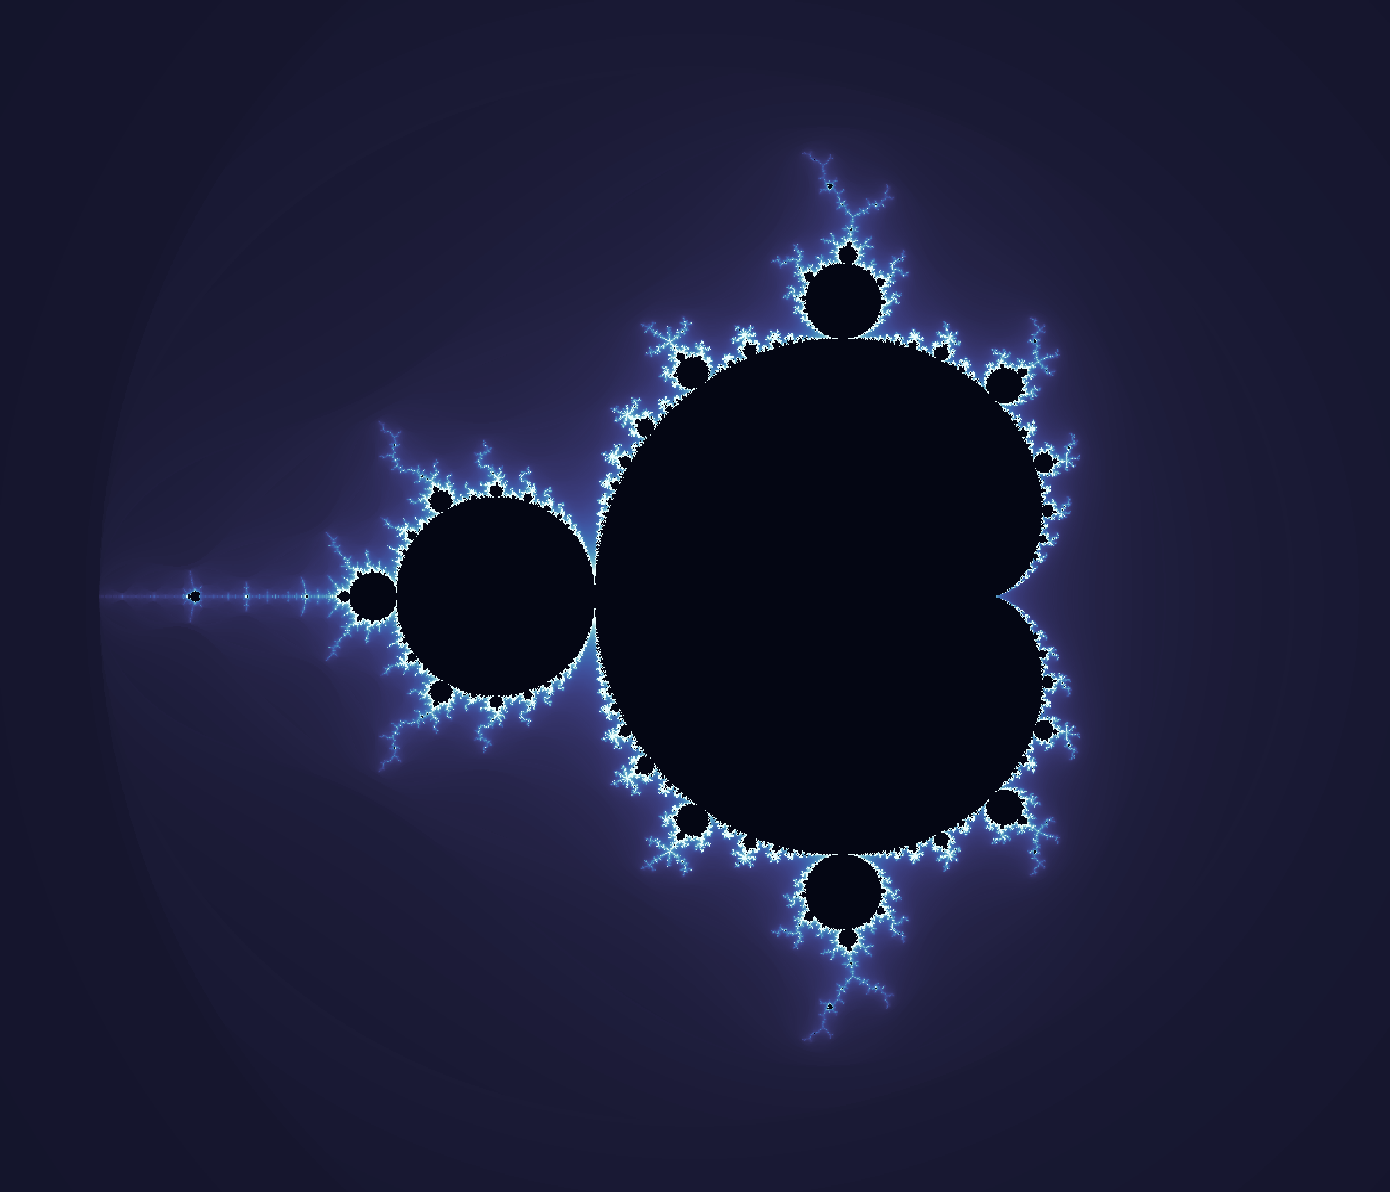
\includegraphics[width=.9\columnwidth]{Mandelbrot_set}
	\end{minipage}

	\vspace{1cm}
\end{frame}

\begin{frame}[t, c]{Examples of fractal objects in nature}{}
	\centering
	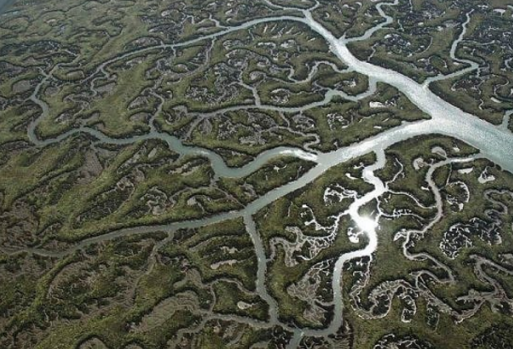
\includegraphics[height=.66\textheight]{image_1}

	\vspace{1cm}
\end{frame}

\begin{frame}[t, c]{Examples of fractal objects in nature}{}
	\centering
	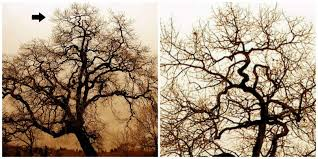
\includegraphics[height=.66\textheight]{image_2}

	\vspace{1cm}
\end{frame}

\begin{frame}[t, c]{Examples of fractal objects in nature}{}
	\centering
	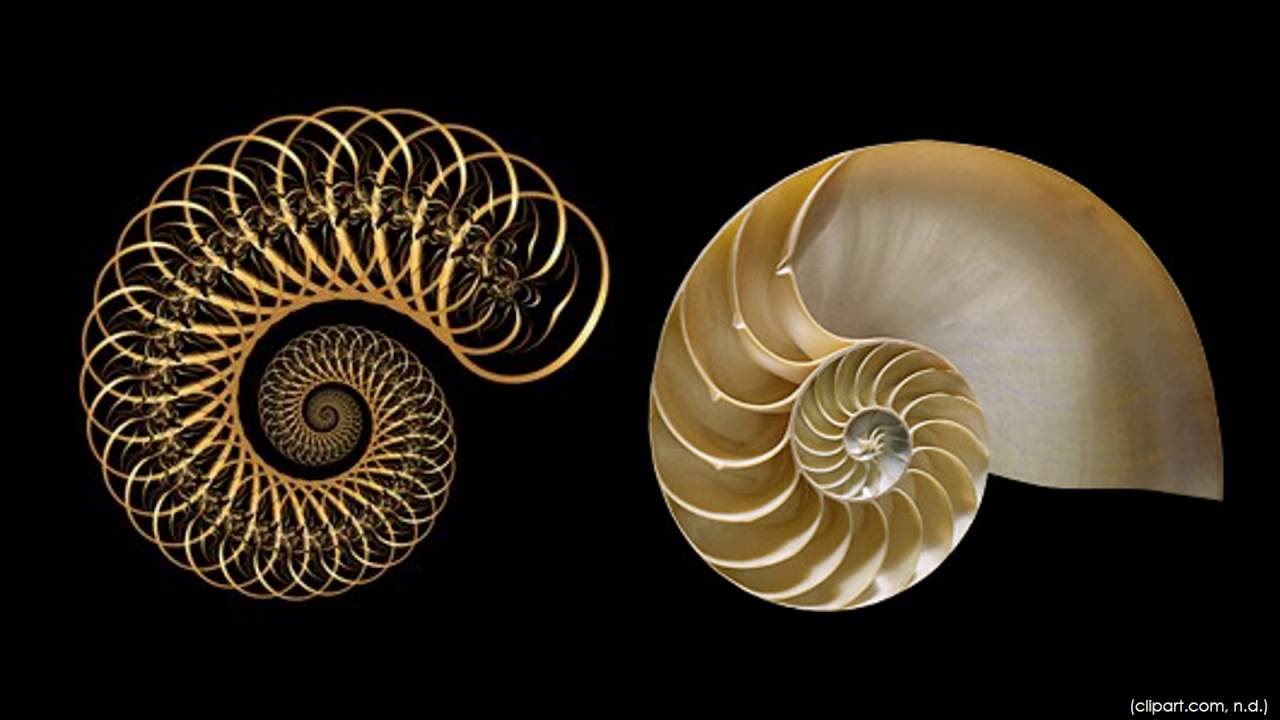
\includegraphics[height=.66\textheight]{image_3}

	\vspace{1cm}
\end{frame}

\begin{frame}[t, c]{Examples of fractal objects in nature}{}
	\centering
	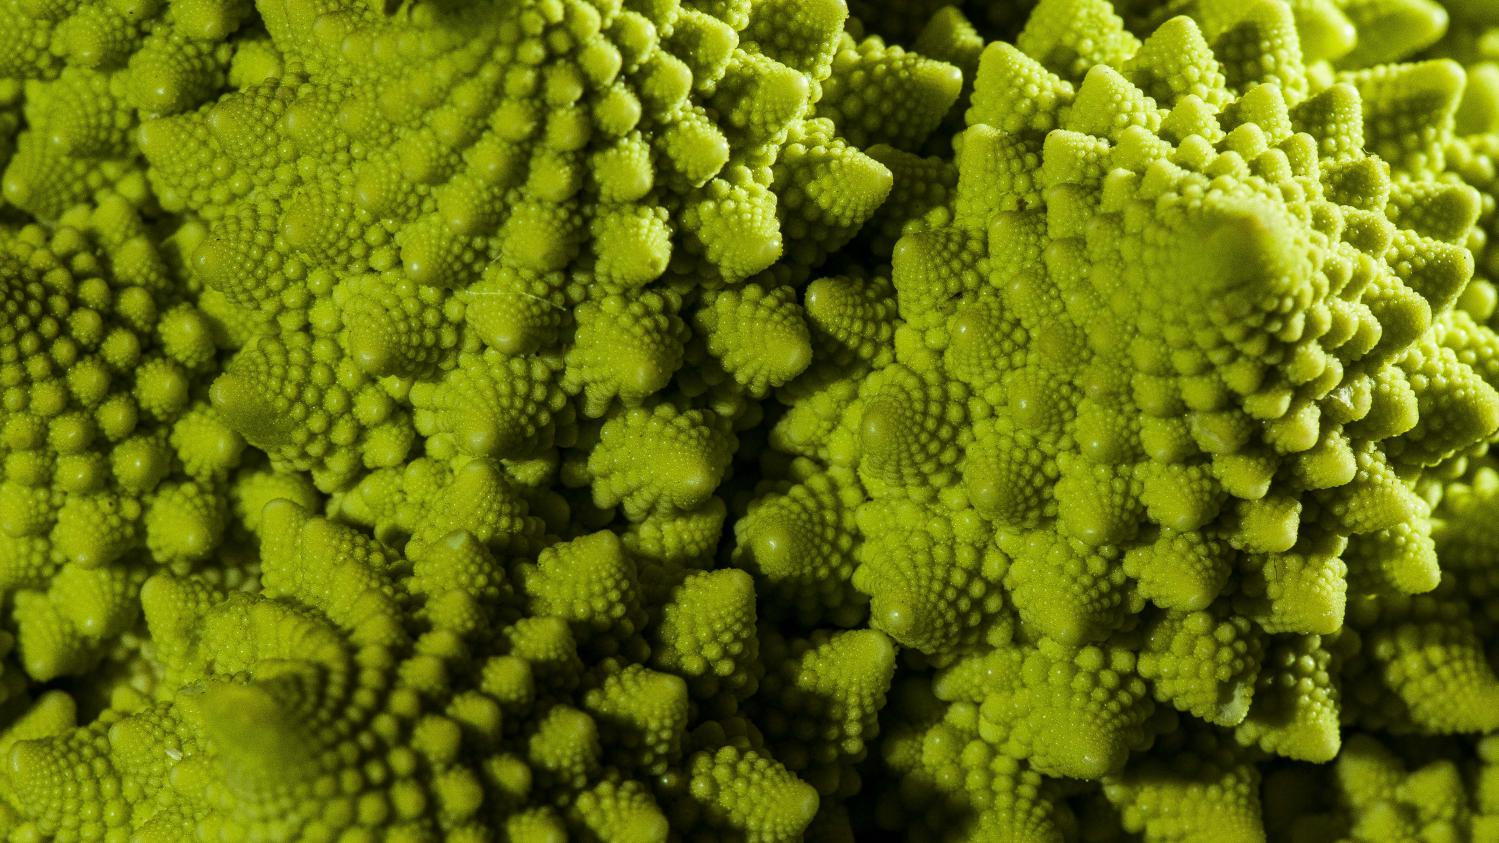
\includegraphics[height=.66\textheight]{image_4}

	\vspace{1cm}
\end{frame}

\begin{frame}[t, c]{Examples of fractal objects in nature}{}
	\centering
	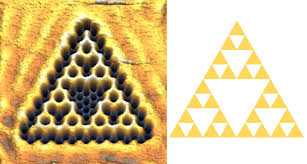
\includegraphics[height=.66\textheight]{image_5}

	\vspace{1cm}
\end{frame}

%-------------------------------------------------------------------------------
%                           QUICK DIVE INTO FRACTAL GEOMETRY
%-------------------------------------------------------------------------------


\begin{frame}[t, c]{}
	\centering
	\vspace{1cm}

	{\Large \textbf{A quick dive into fractal geometry}}

	\bigskip

	{\textgre{\textbf{Cantor set, Koch snow flake and non-integer dimensions}}}

\end{frame}

\begin{frame}[t, c]{Koch snow flake}{A finite area within an infinite perimeter?}
	Koch snow flake can easily be constructed by starting with an equilateral triangle as follows:
	\begin{enumerate}
		\item Divide the line segment into three segments of equal length.
		\item Draw an equilateral triangle that has the middle segment from step 1 as its based points outward.
		\item Remove the line segment that is the base of the triangle from step 2.
	\end{enumerate}

	\vspace{1cm}
\end{frame}

\begin{frame}[t, c]{Koch snow flake}{A finite area within an infinite perimeter?}
	\centering
	\begin{minipage}{.48\textwidth}
		\begin{itemize}
			\item At the 0\textsuperscript{th} iteration:
			\begin{itemize}
				\item[$\hookrightarrow$] $N_0 = 3$
				\item[$\hookrightarrow$] $S_0 = 1$
			\end{itemize}

			\bigskip

			\item We'll work out the area later.
		\end{itemize}
	\end{minipage}%
	\hfill
	\begin{minipage}{.48\textwidth}
		\centering
		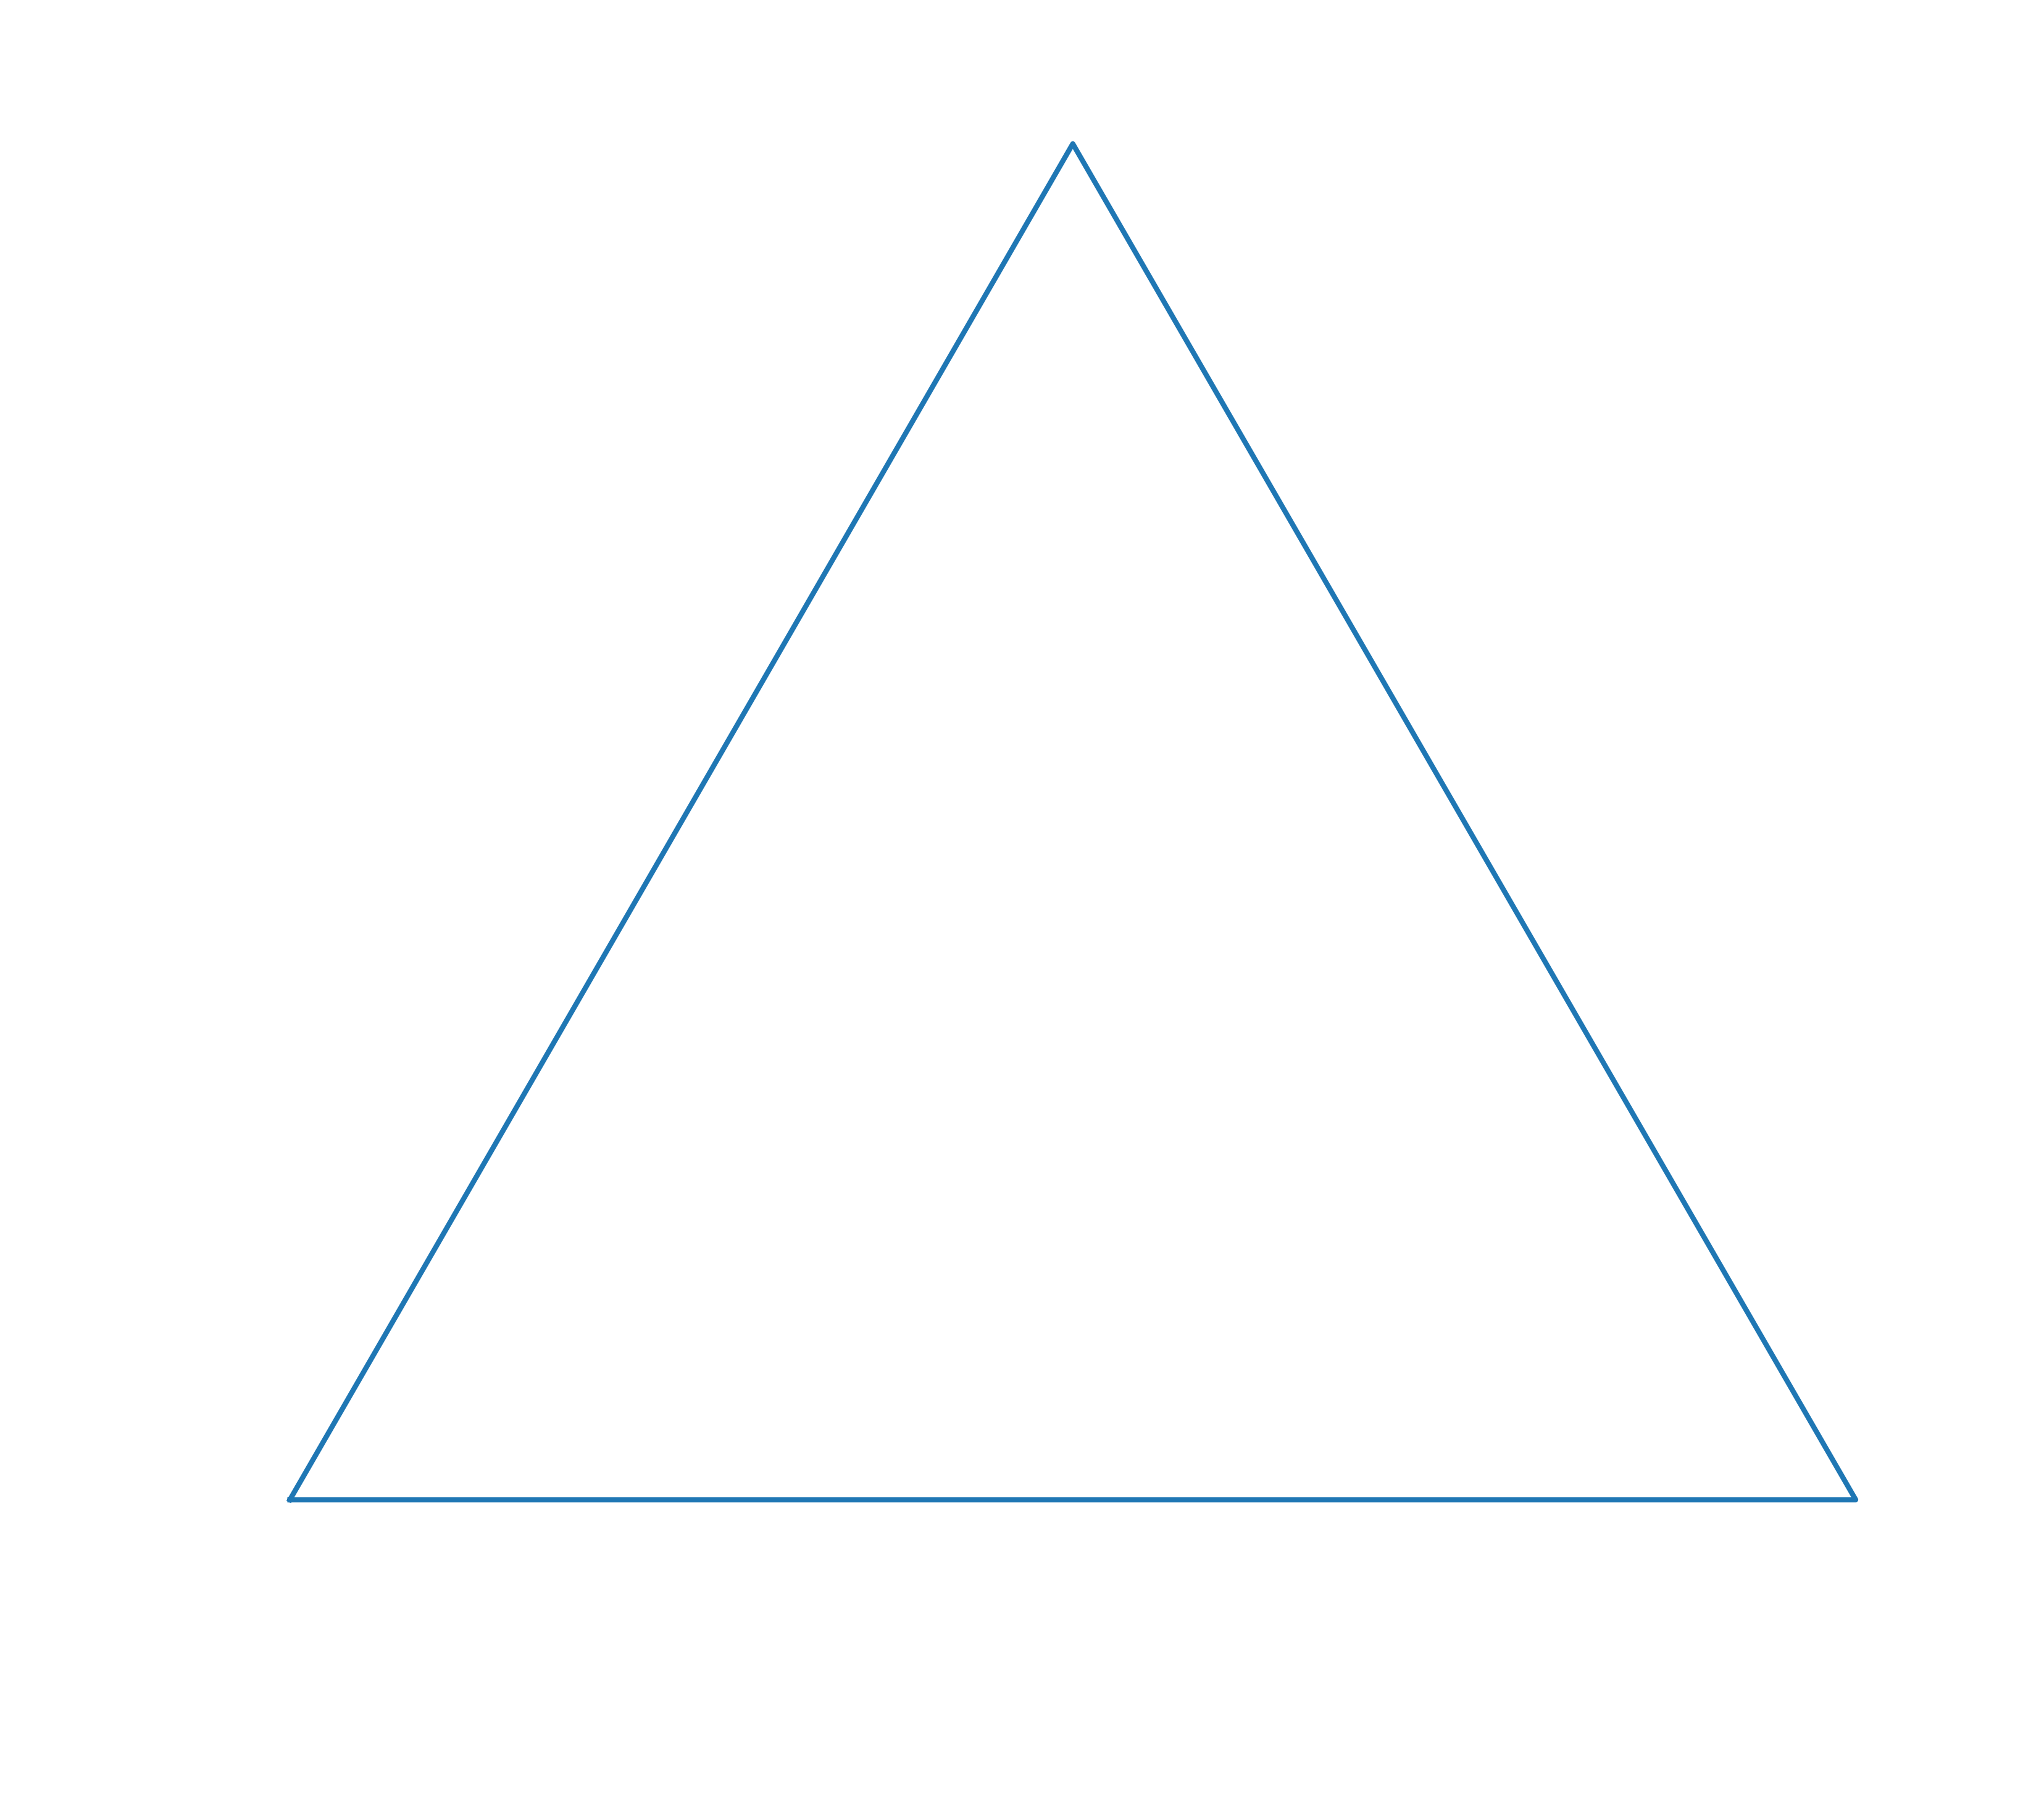
\includegraphics[width=.8\textwidth]{koch_0_it}
	\end{minipage}

	\vspace{1cm}
\end{frame}

\begin{frame}[t, c]{Koch snow flake}{A finite area within an infinite perimeter?}
	\centering
	\begin{minipage}{.48\textwidth}
		\begin{itemize}
			\item At the 1\textsuperscript{st} iteration:
			\begin{itemize}
				\item[$\hookrightarrow$] $N_1 = 3 \times 4$
				\item[$\hookrightarrow$] $S_1 = \nicefrac{1}{3}$
			\end{itemize}

			\bigskip

			\item We'll work out the area later.
		\end{itemize}
	\end{minipage}%
	\hfill
	\begin{minipage}{.48\textwidth}
		\centering
		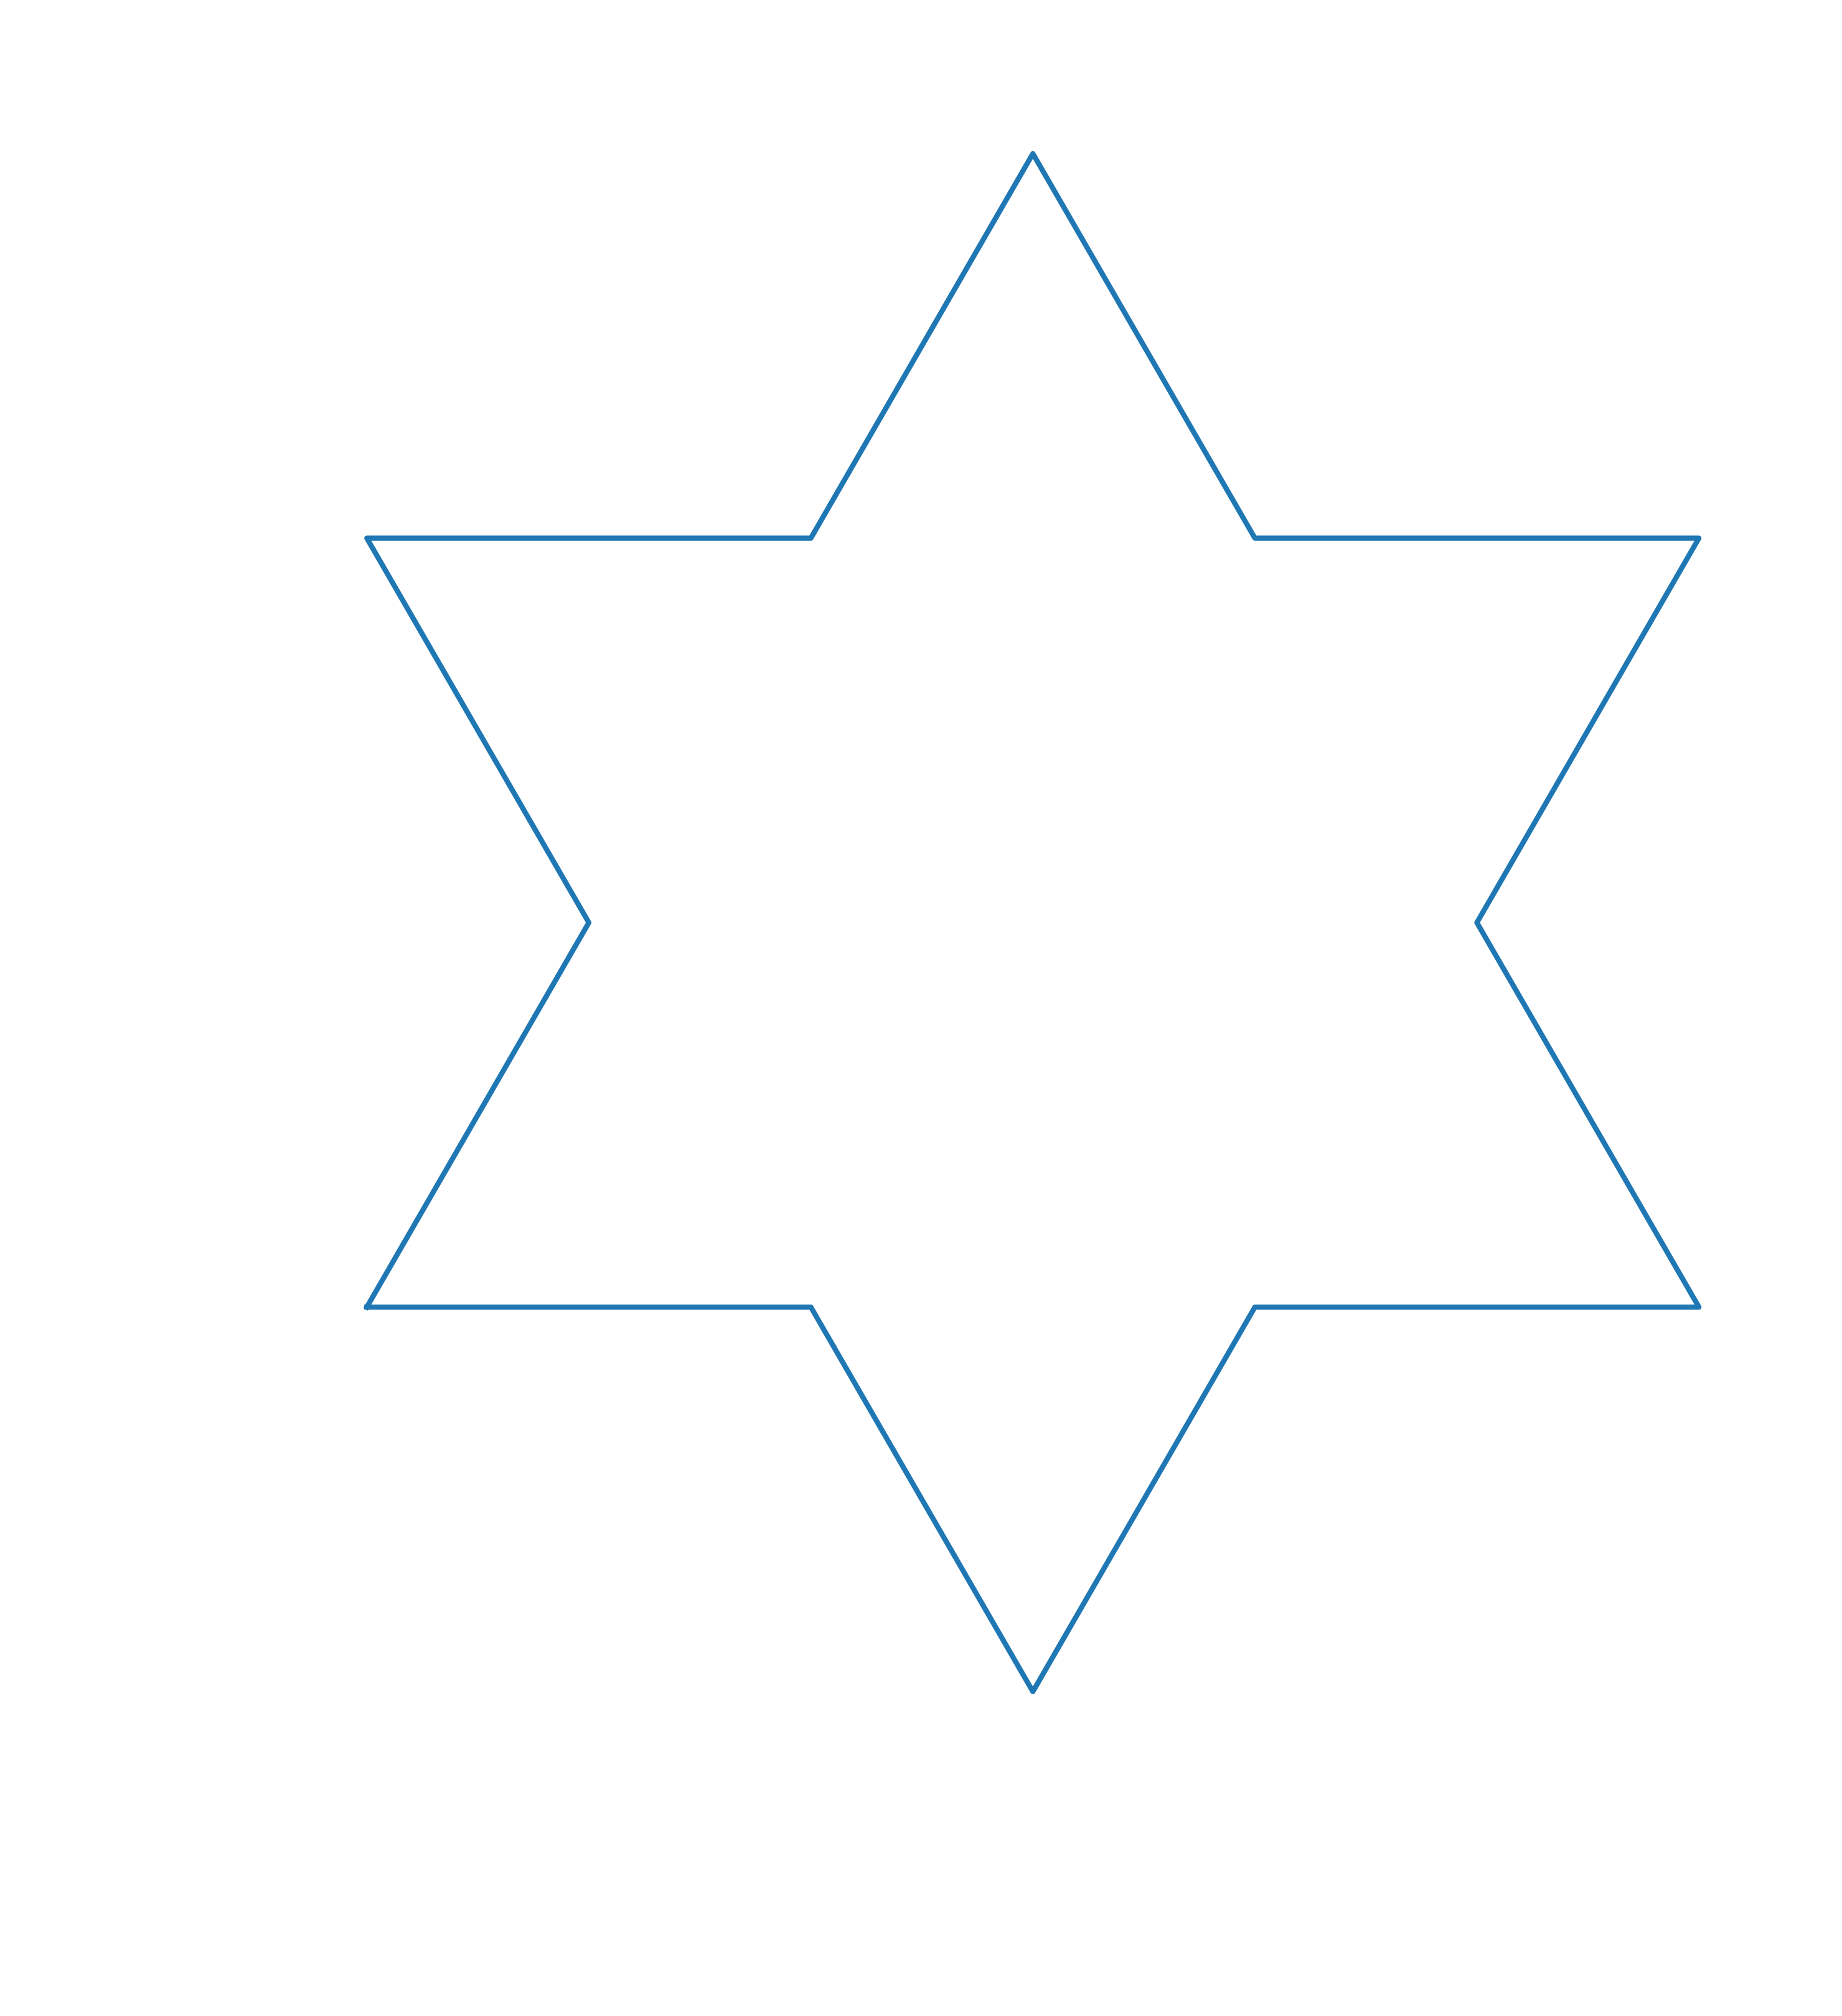
\includegraphics[width=.8\textwidth]{koch_1_it}
	\end{minipage}

	\vspace{1cm}
\end{frame}

\begin{frame}[t, c]{Koch snow flake}{A finite area within an infinite perimeter?}
	\centering
	\begin{minipage}{.48\textwidth}
		\begin{itemize}
			\item At the 2\textsuperscript{nd} iteration:
			\begin{itemize}
				\item[$\hookrightarrow$] $N_2 = 3 \times 4^2$
				\item[$\hookrightarrow$] $S_2 = \nicefrac{1}{3^2}$
			\end{itemize}

			\bigskip

			\item We'll work out the area later.
		\end{itemize}
	\end{minipage}%
	\hfill
	\begin{minipage}{.48\textwidth}
		\centering
		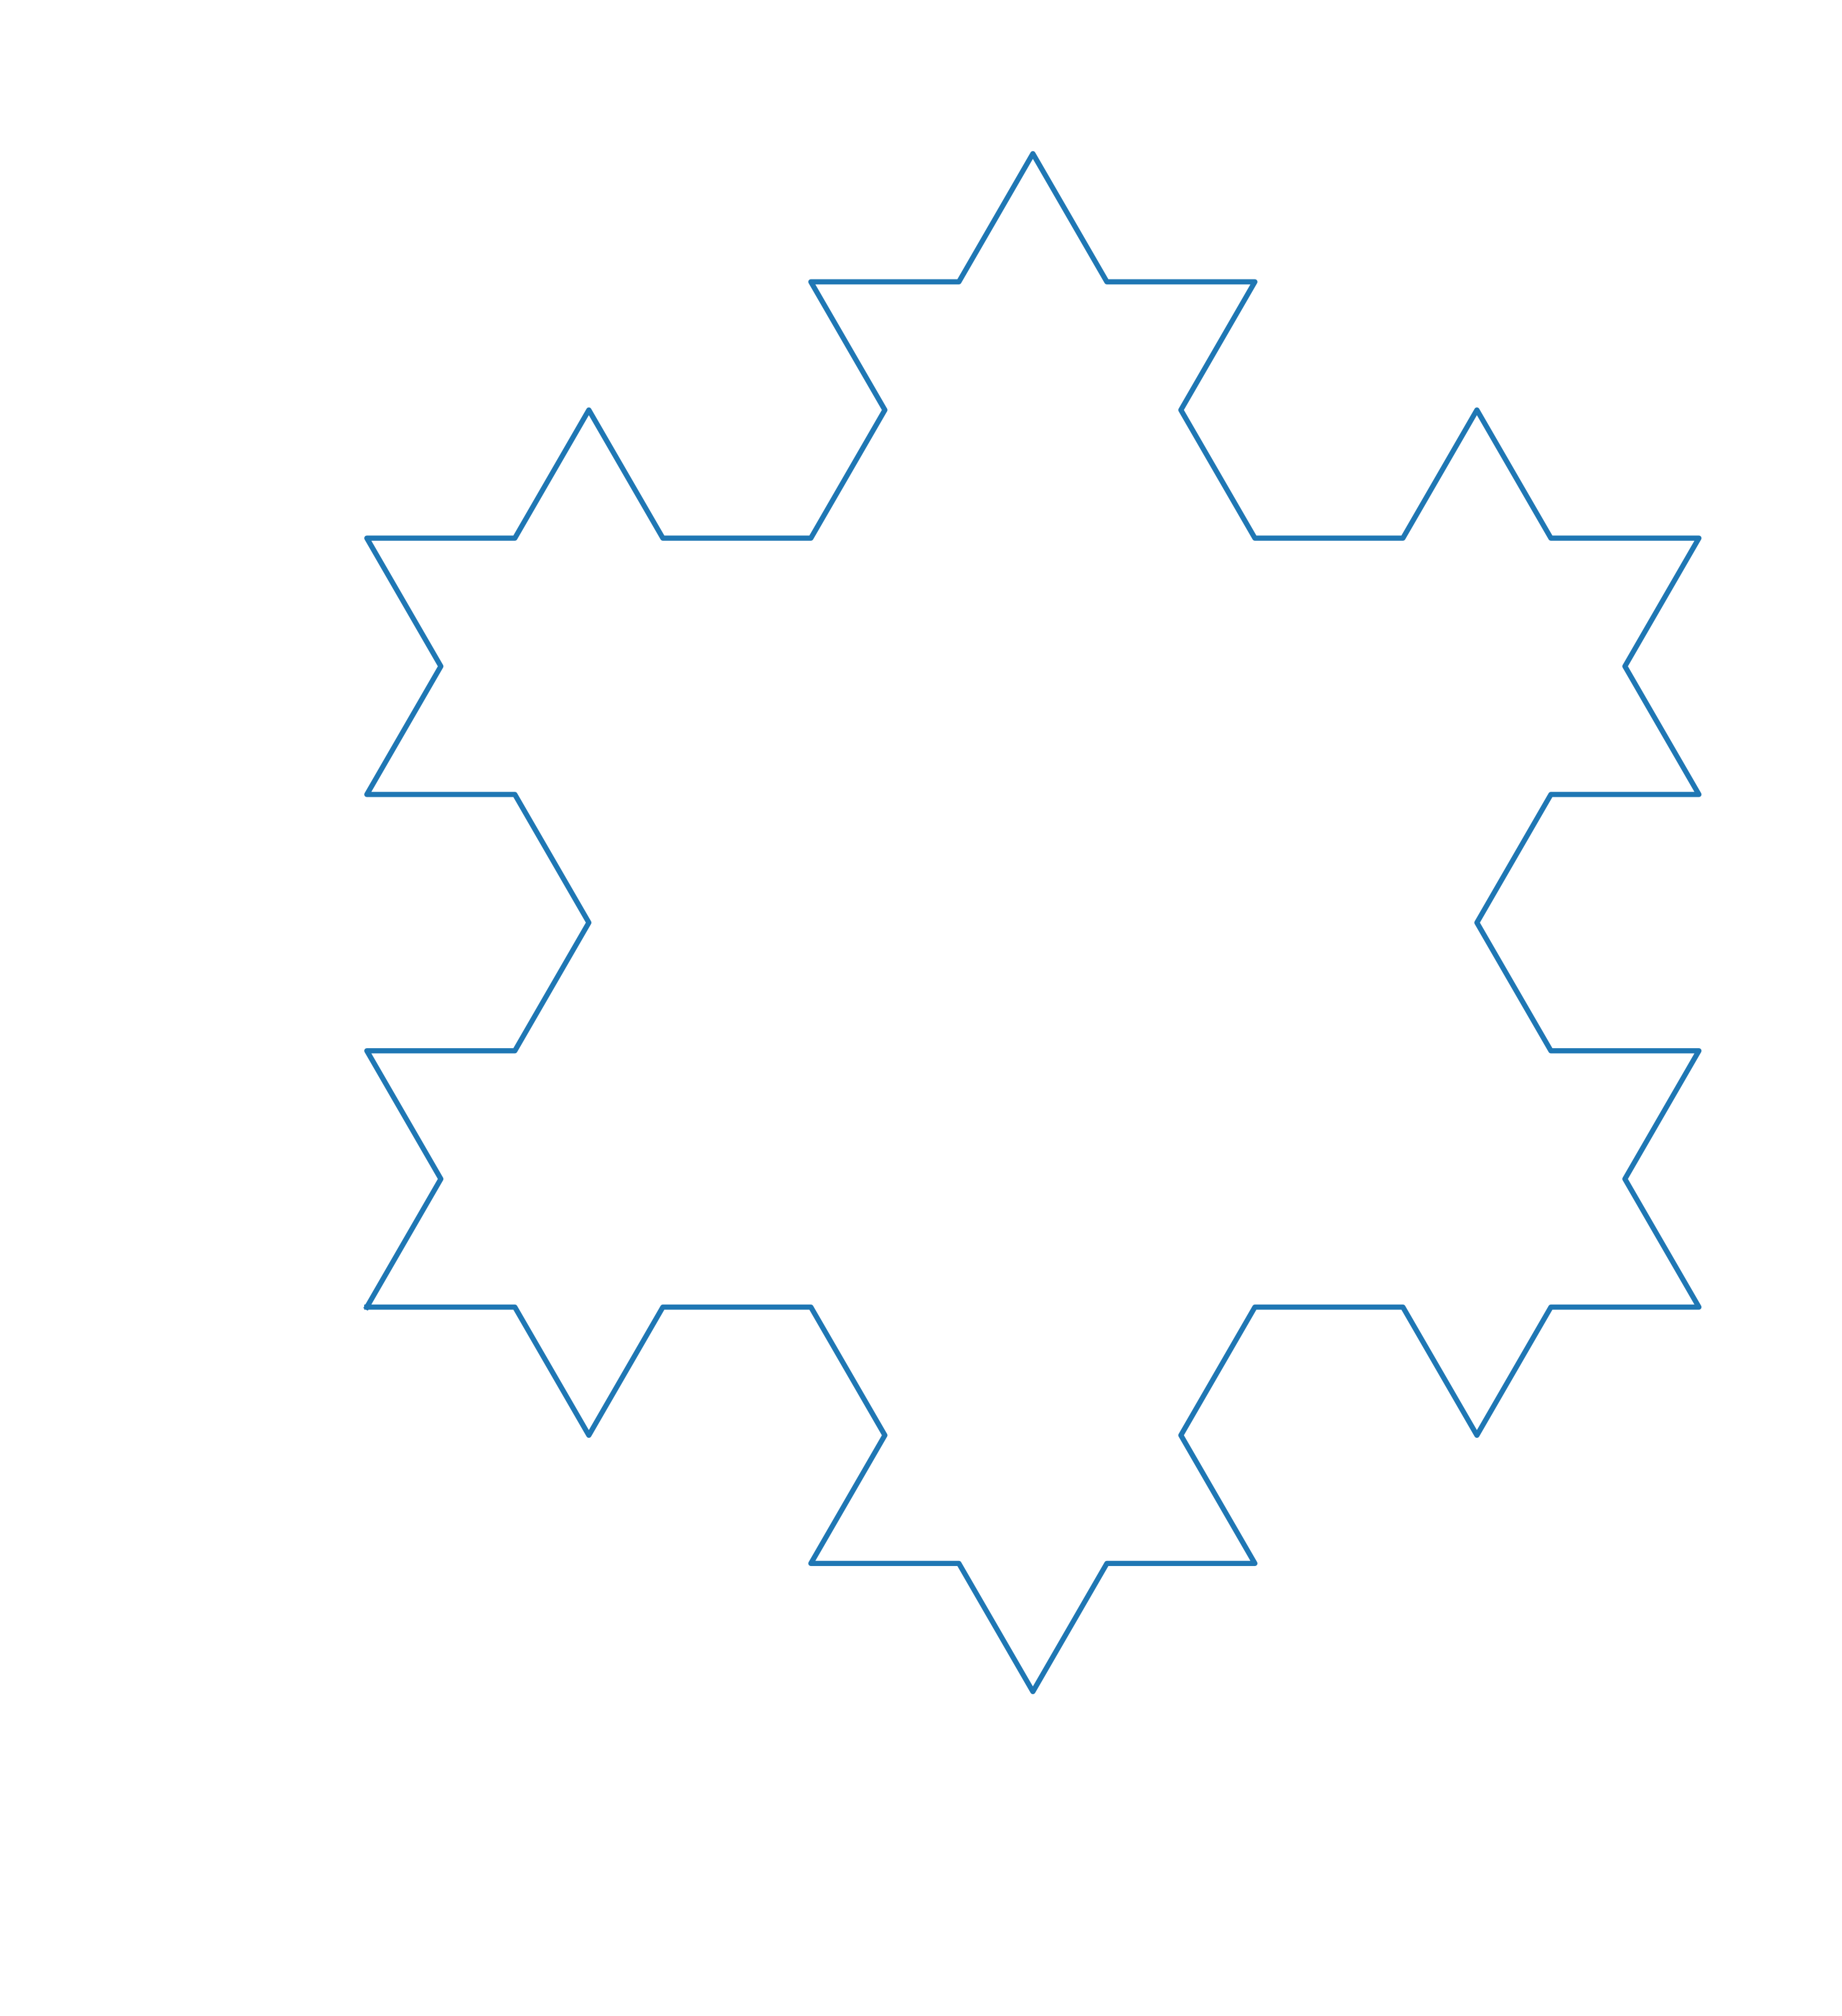
\includegraphics[width=.8\textwidth]{koch_2_it}
	\end{minipage}

	\vspace{1cm}
\end{frame}

\begin{frame}[t, c]{Koch snow flake}{A finite area within an infinite perimeter?}
	\centering
	\begin{minipage}{.48\textwidth}
		\begin{itemize}
			\item At the 3\textsuperscript{rd} iteration:
			\begin{itemize}
				\item[$\hookrightarrow$] $N_3 = 3 \times 4^3$
				\item[$\hookrightarrow$] $S_3 = \nicefrac{1}{3^3}$
			\end{itemize}

			\bigskip

			\item We'll work out the area later.
		\end{itemize}
	\end{minipage}%
	\hfill
	\begin{minipage}{.48\textwidth}
		\centering
		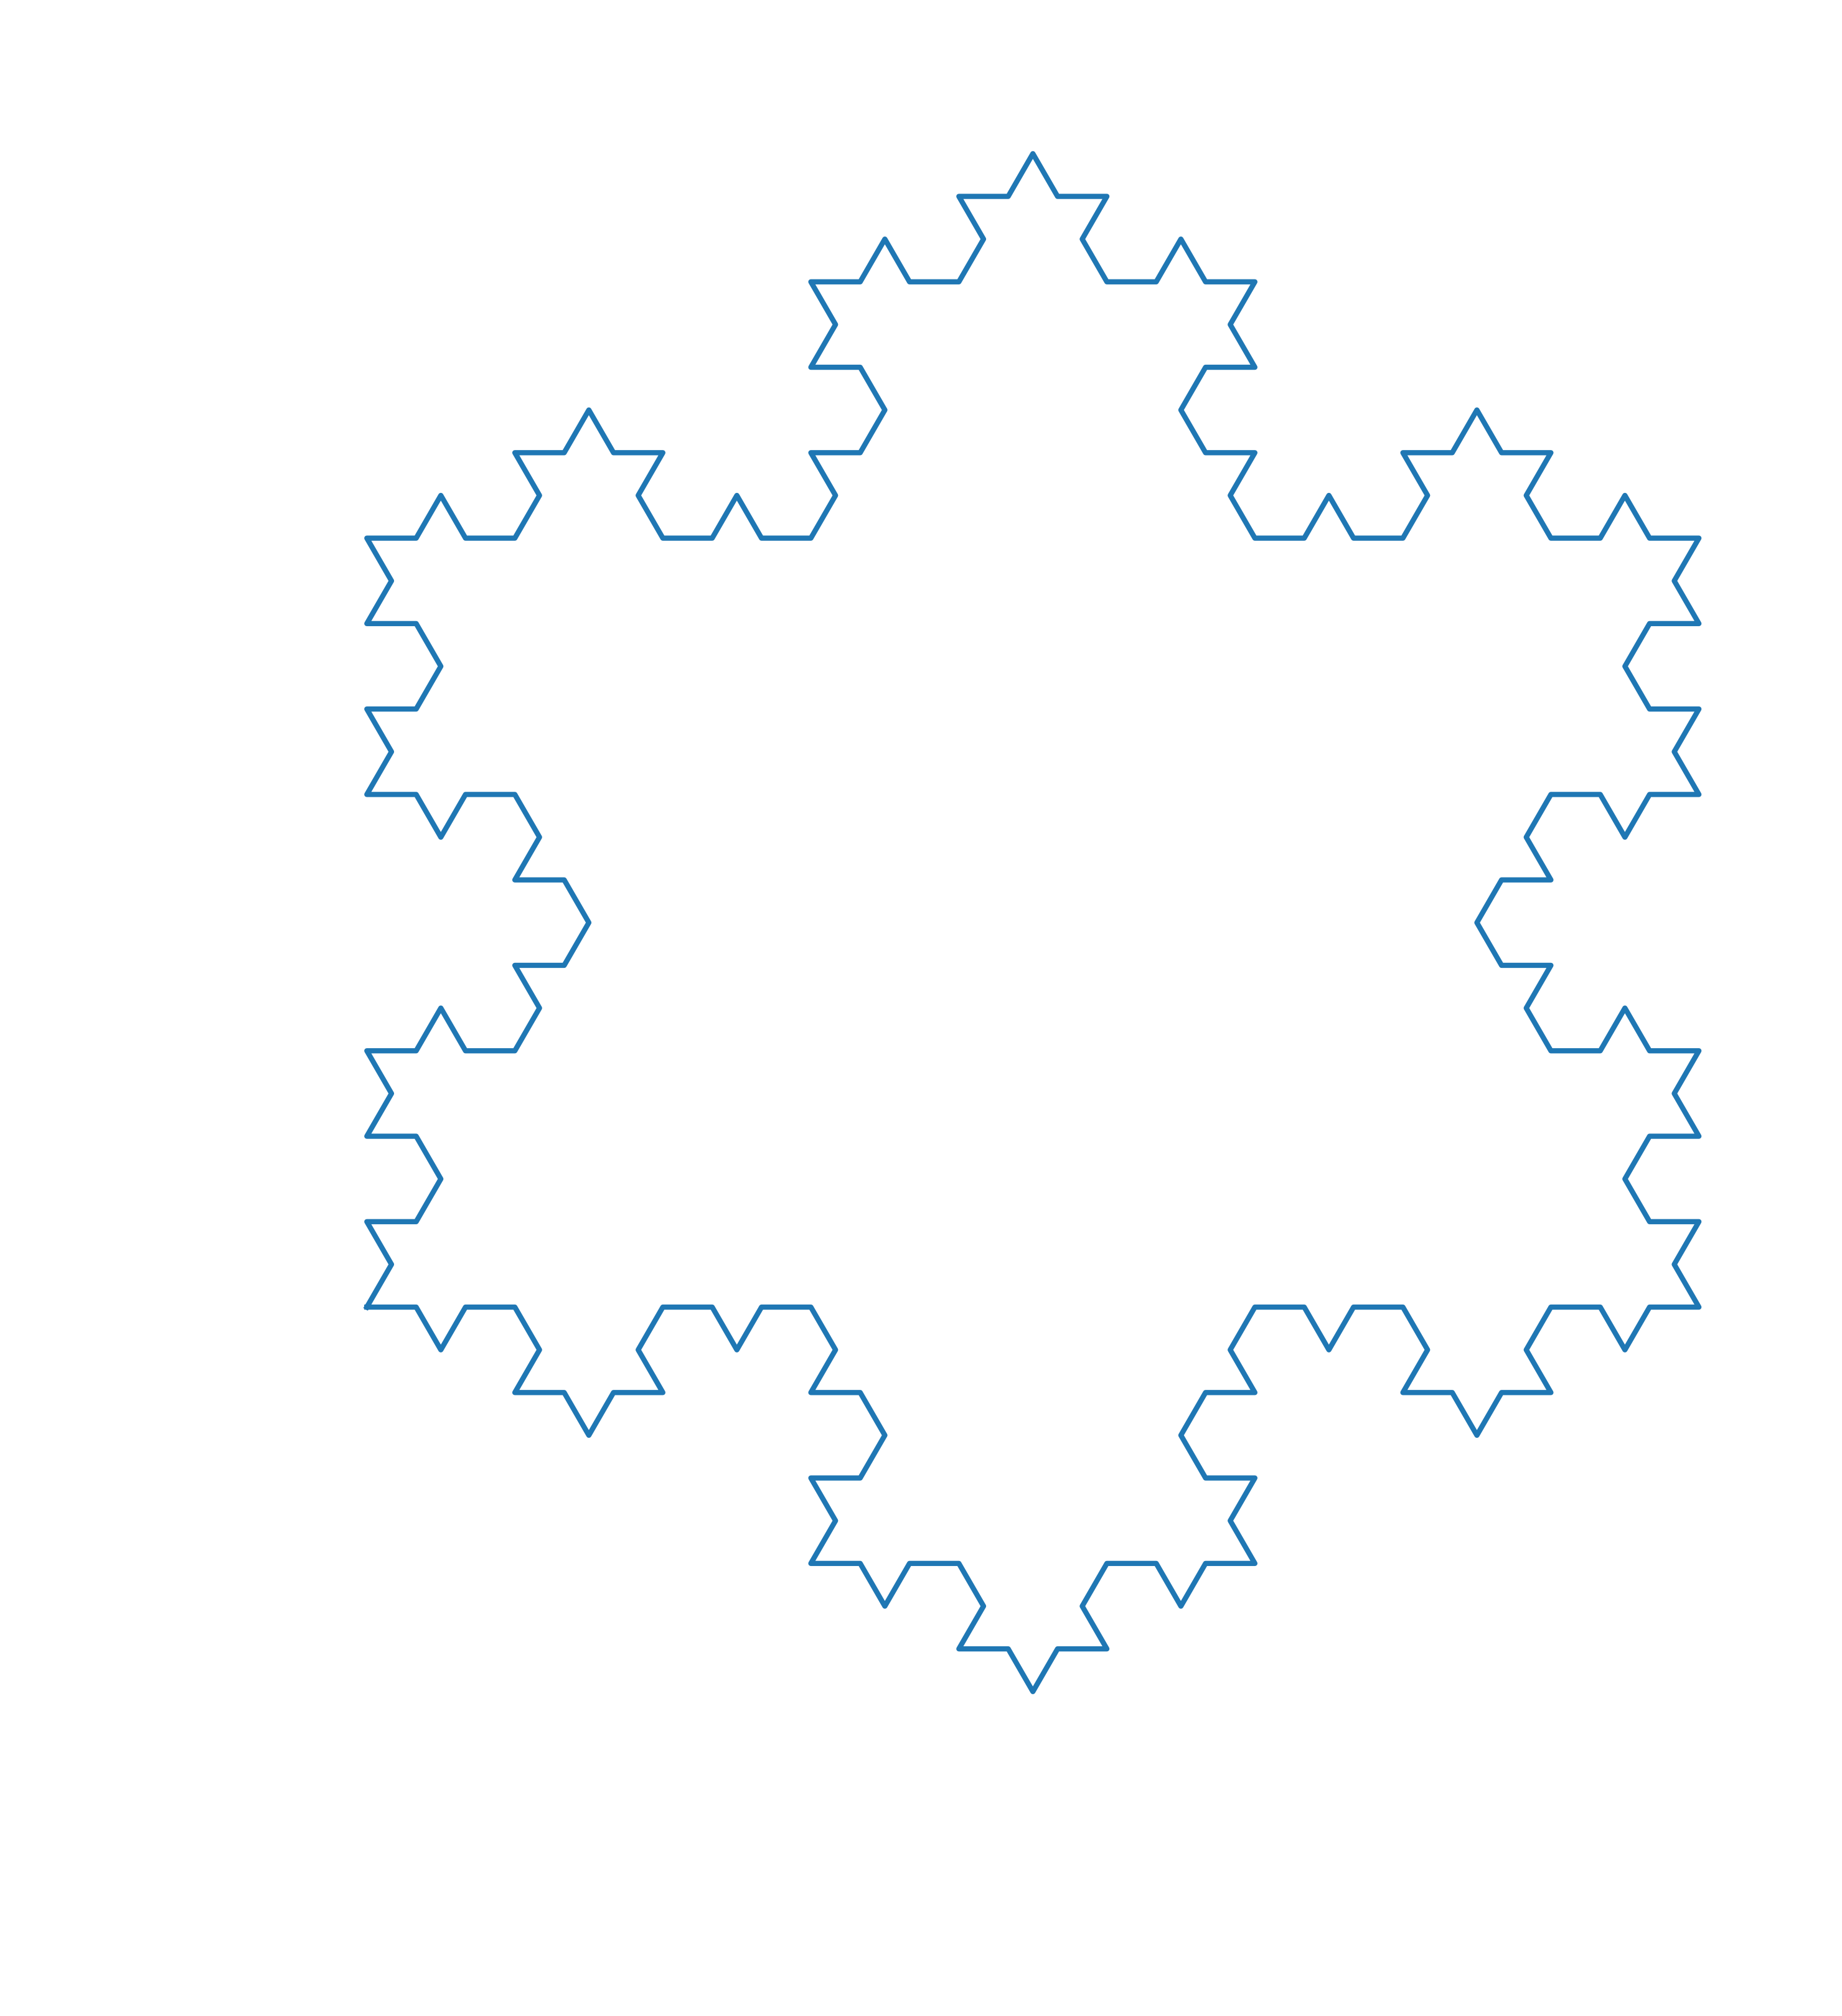
\includegraphics[width=.8\textwidth]{koch_3_it}
	\end{minipage}

	\vspace{1cm}
\end{frame}

\begin{frame}[t, c]{Koch snow flake}{A finite area within an infinite perimeter?}
	\centering
	\begin{minipage}{.48\textwidth}
		\begin{itemize}
			\item At the 4\textsuperscript{th} iteration:
			\begin{itemize}
				\item[$\hookrightarrow$] $N_4 = 3 \times 4^4$
				\item[$\hookrightarrow$] $S_4 = \nicefrac{1}{3^4}$
			\end{itemize}

			\bigskip

			\item We'll work out the area later.
		\end{itemize}
	\end{minipage}%
	\hfill
	\begin{minipage}{.48\textwidth}
		\centering
		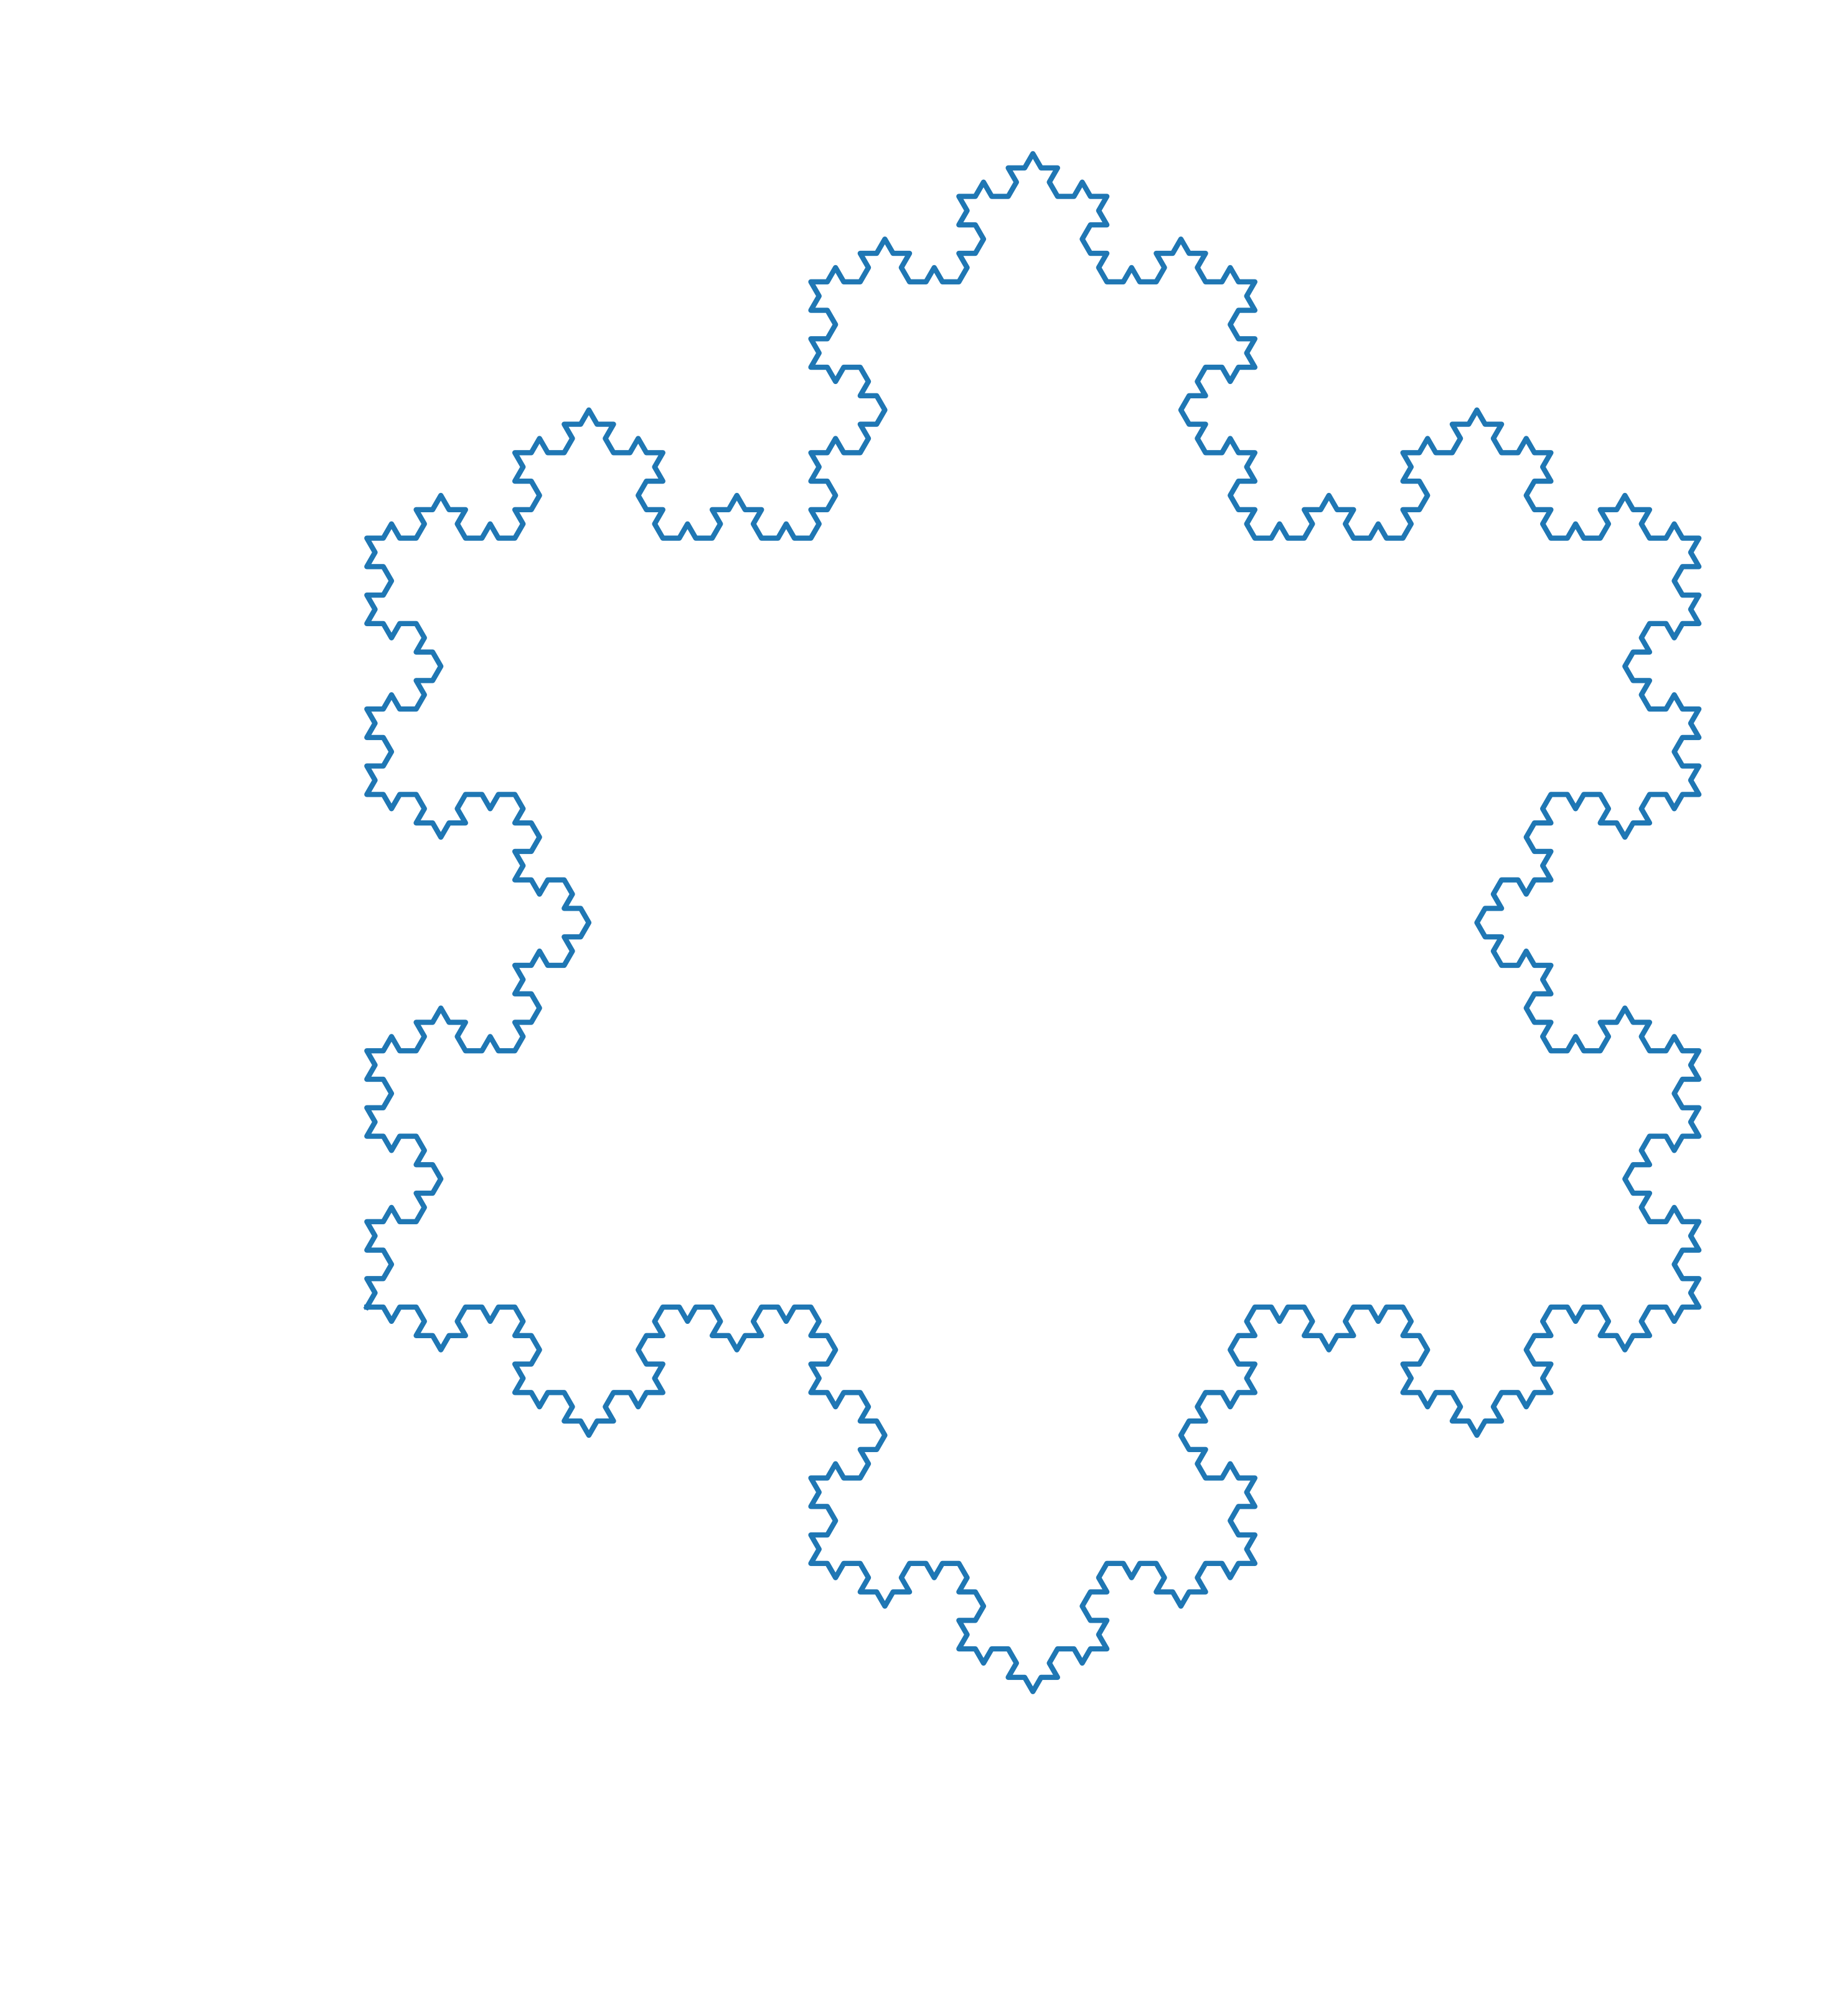
\includegraphics[width=.8\textwidth]{koch_4_it}
	\end{minipage}

	\vspace{1cm}
\end{frame}

\begin{frame}[t, c]{Koch snow flake}{A finite area within an infinite perimeter?}
	\centering
	\begin{minipage}{.48\textwidth}
		\begin{itemize}
			\item At the 5\textsuperscript{th} iteration:
			\begin{itemize}
				\item[$\hookrightarrow$] $N_5 = 3 \times 4^5$
				\item[$\hookrightarrow$] $S_5 = \nicefrac{1}{3^5}$
			\end{itemize}

			\bigskip

			\item We'll work out the area later.
		\end{itemize}
	\end{minipage}%
	\hfill
	\begin{minipage}{.48\textwidth}
		\centering
		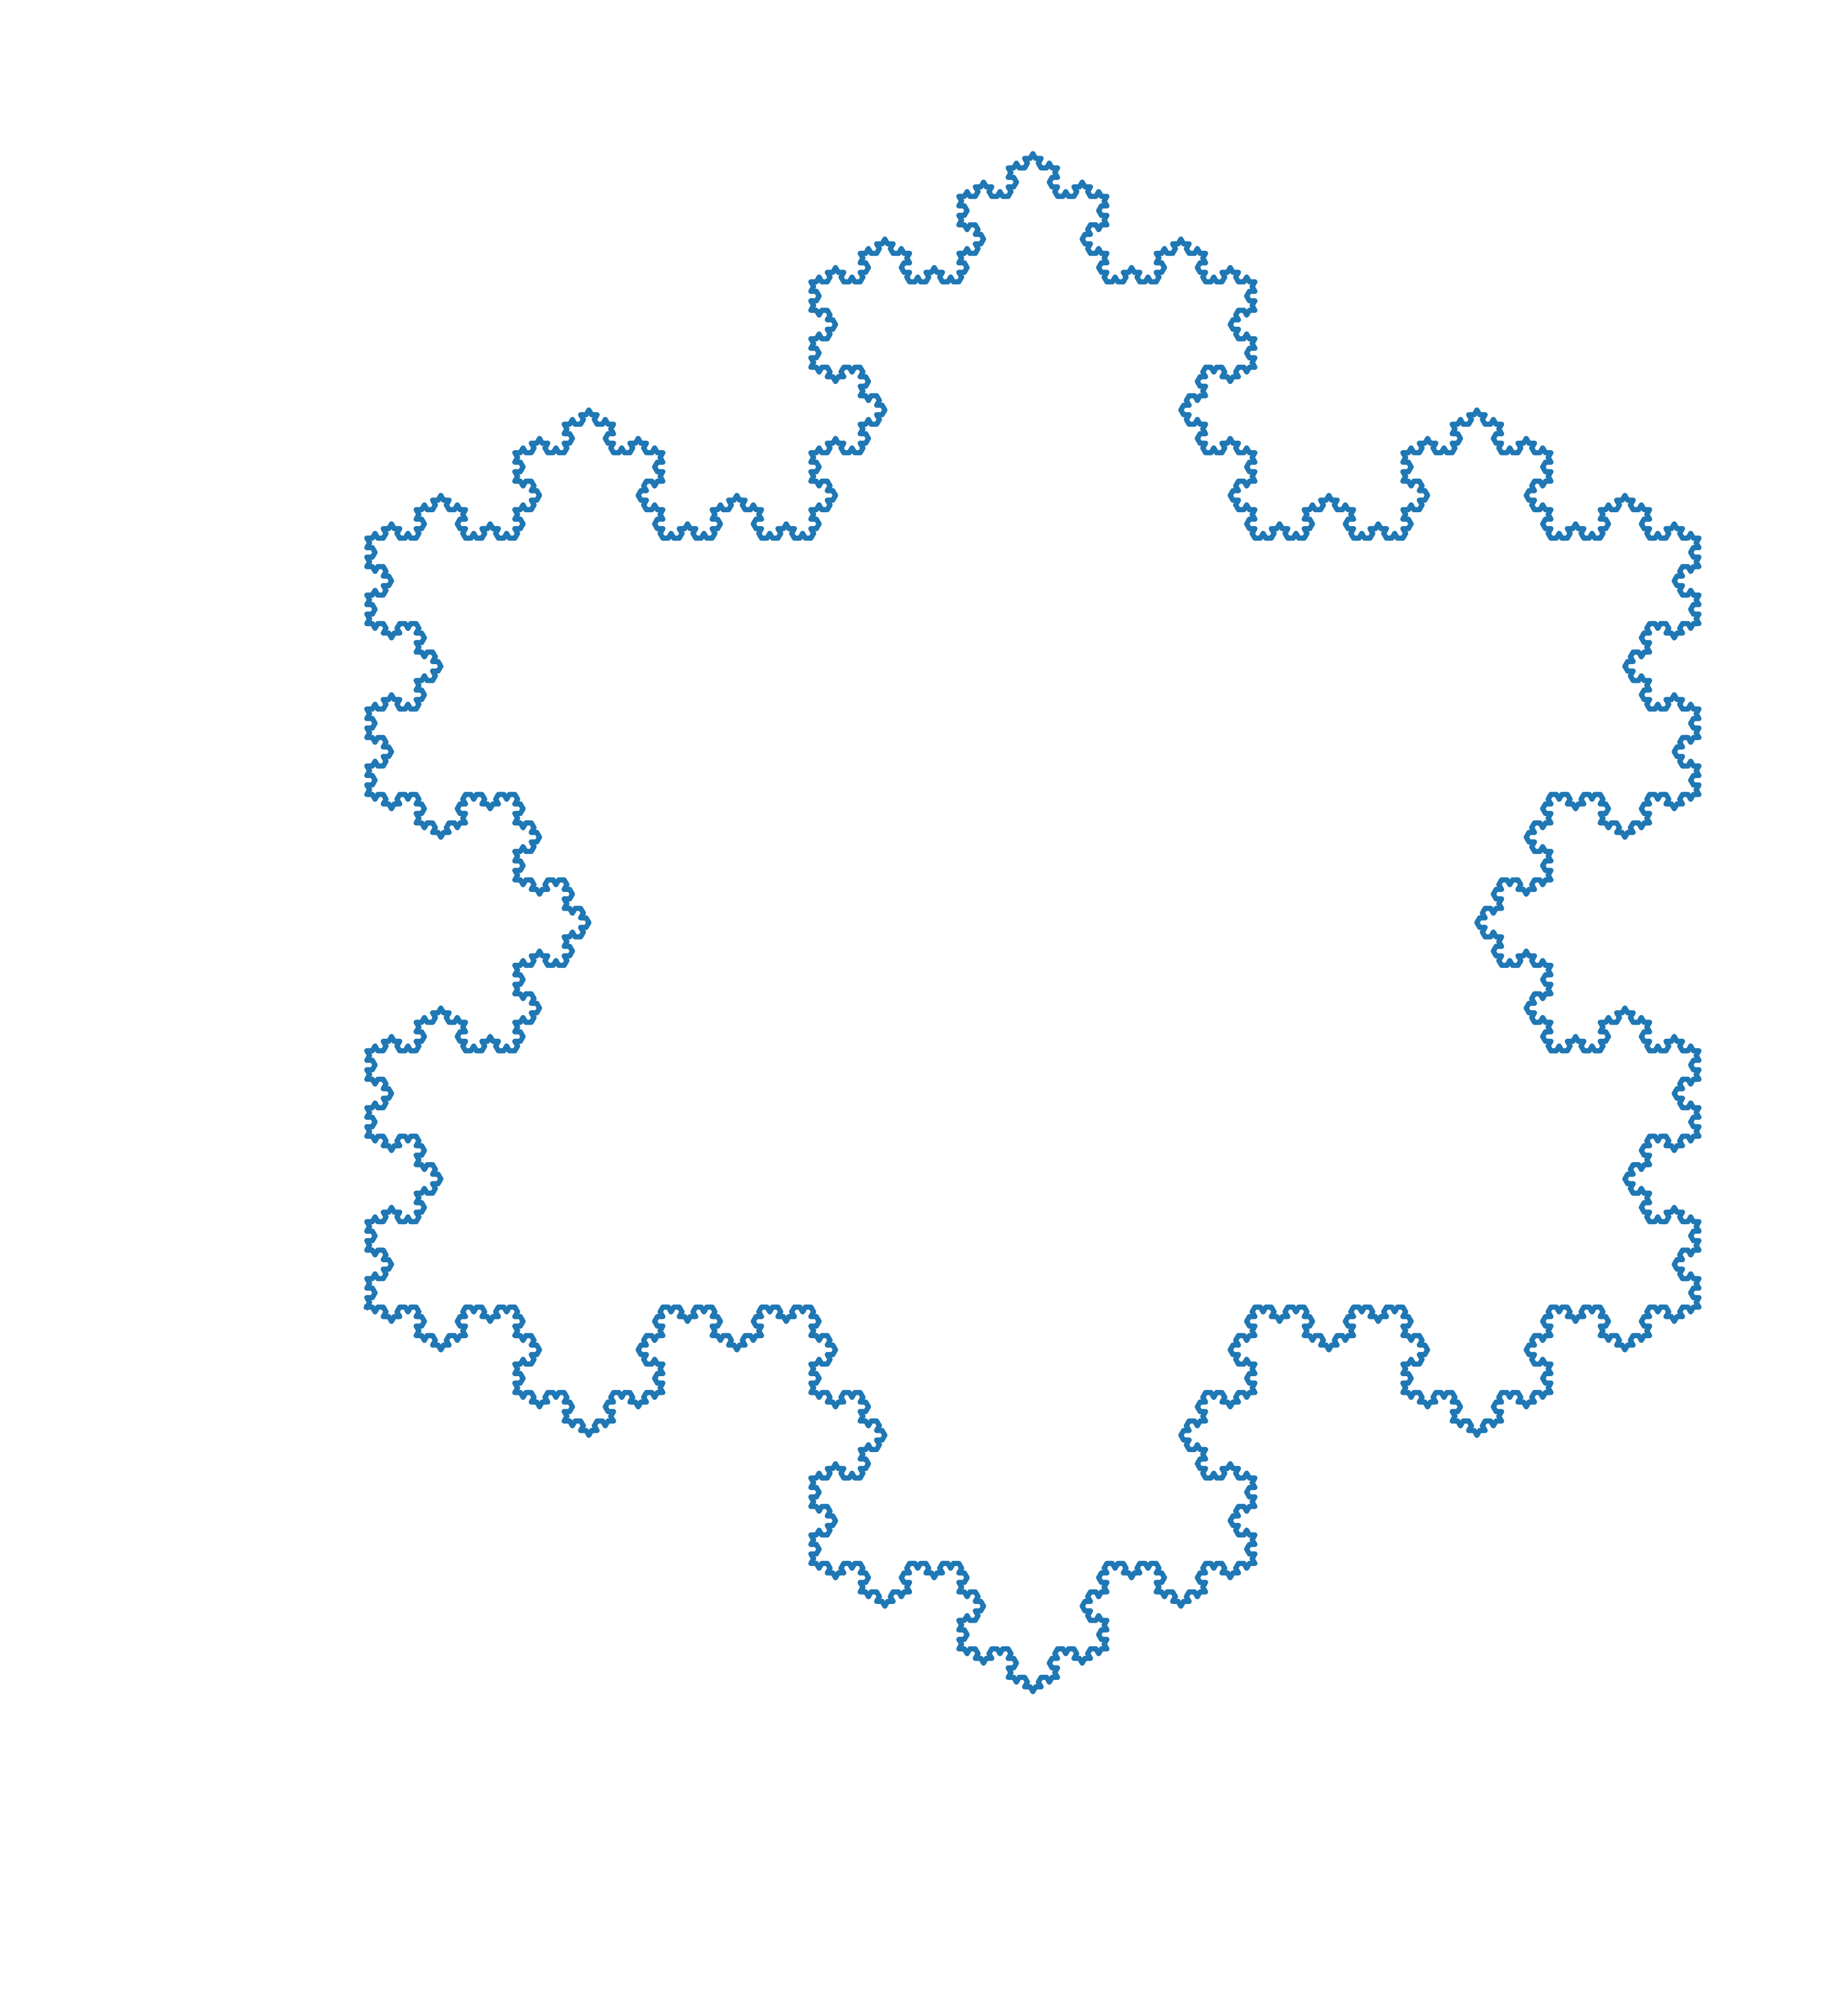
\includegraphics[width=.8\textwidth]{koch_5_it}
	\end{minipage}

	\vspace{1cm}
\end{frame}

\begin{frame}[t, c]{Koch snow flake}{A finite area within an infinite perimeter?}
	\centering
	\begin{minipage}{.48\textwidth}
		\begin{itemize}
			\item At the 6\textsuperscript{th} iteration:
			\begin{itemize}
				\item[$\hookrightarrow$] $N_6 = 3 \times 4^6$
				\item[$\hookrightarrow$] $S_6 = \nicefrac{1}{3^6}$
			\end{itemize}

			\bigskip

			\item We'll work out the area later.
		\end{itemize}
	\end{minipage}%
	\hfill
	\begin{minipage}{.48\textwidth}
		\centering
		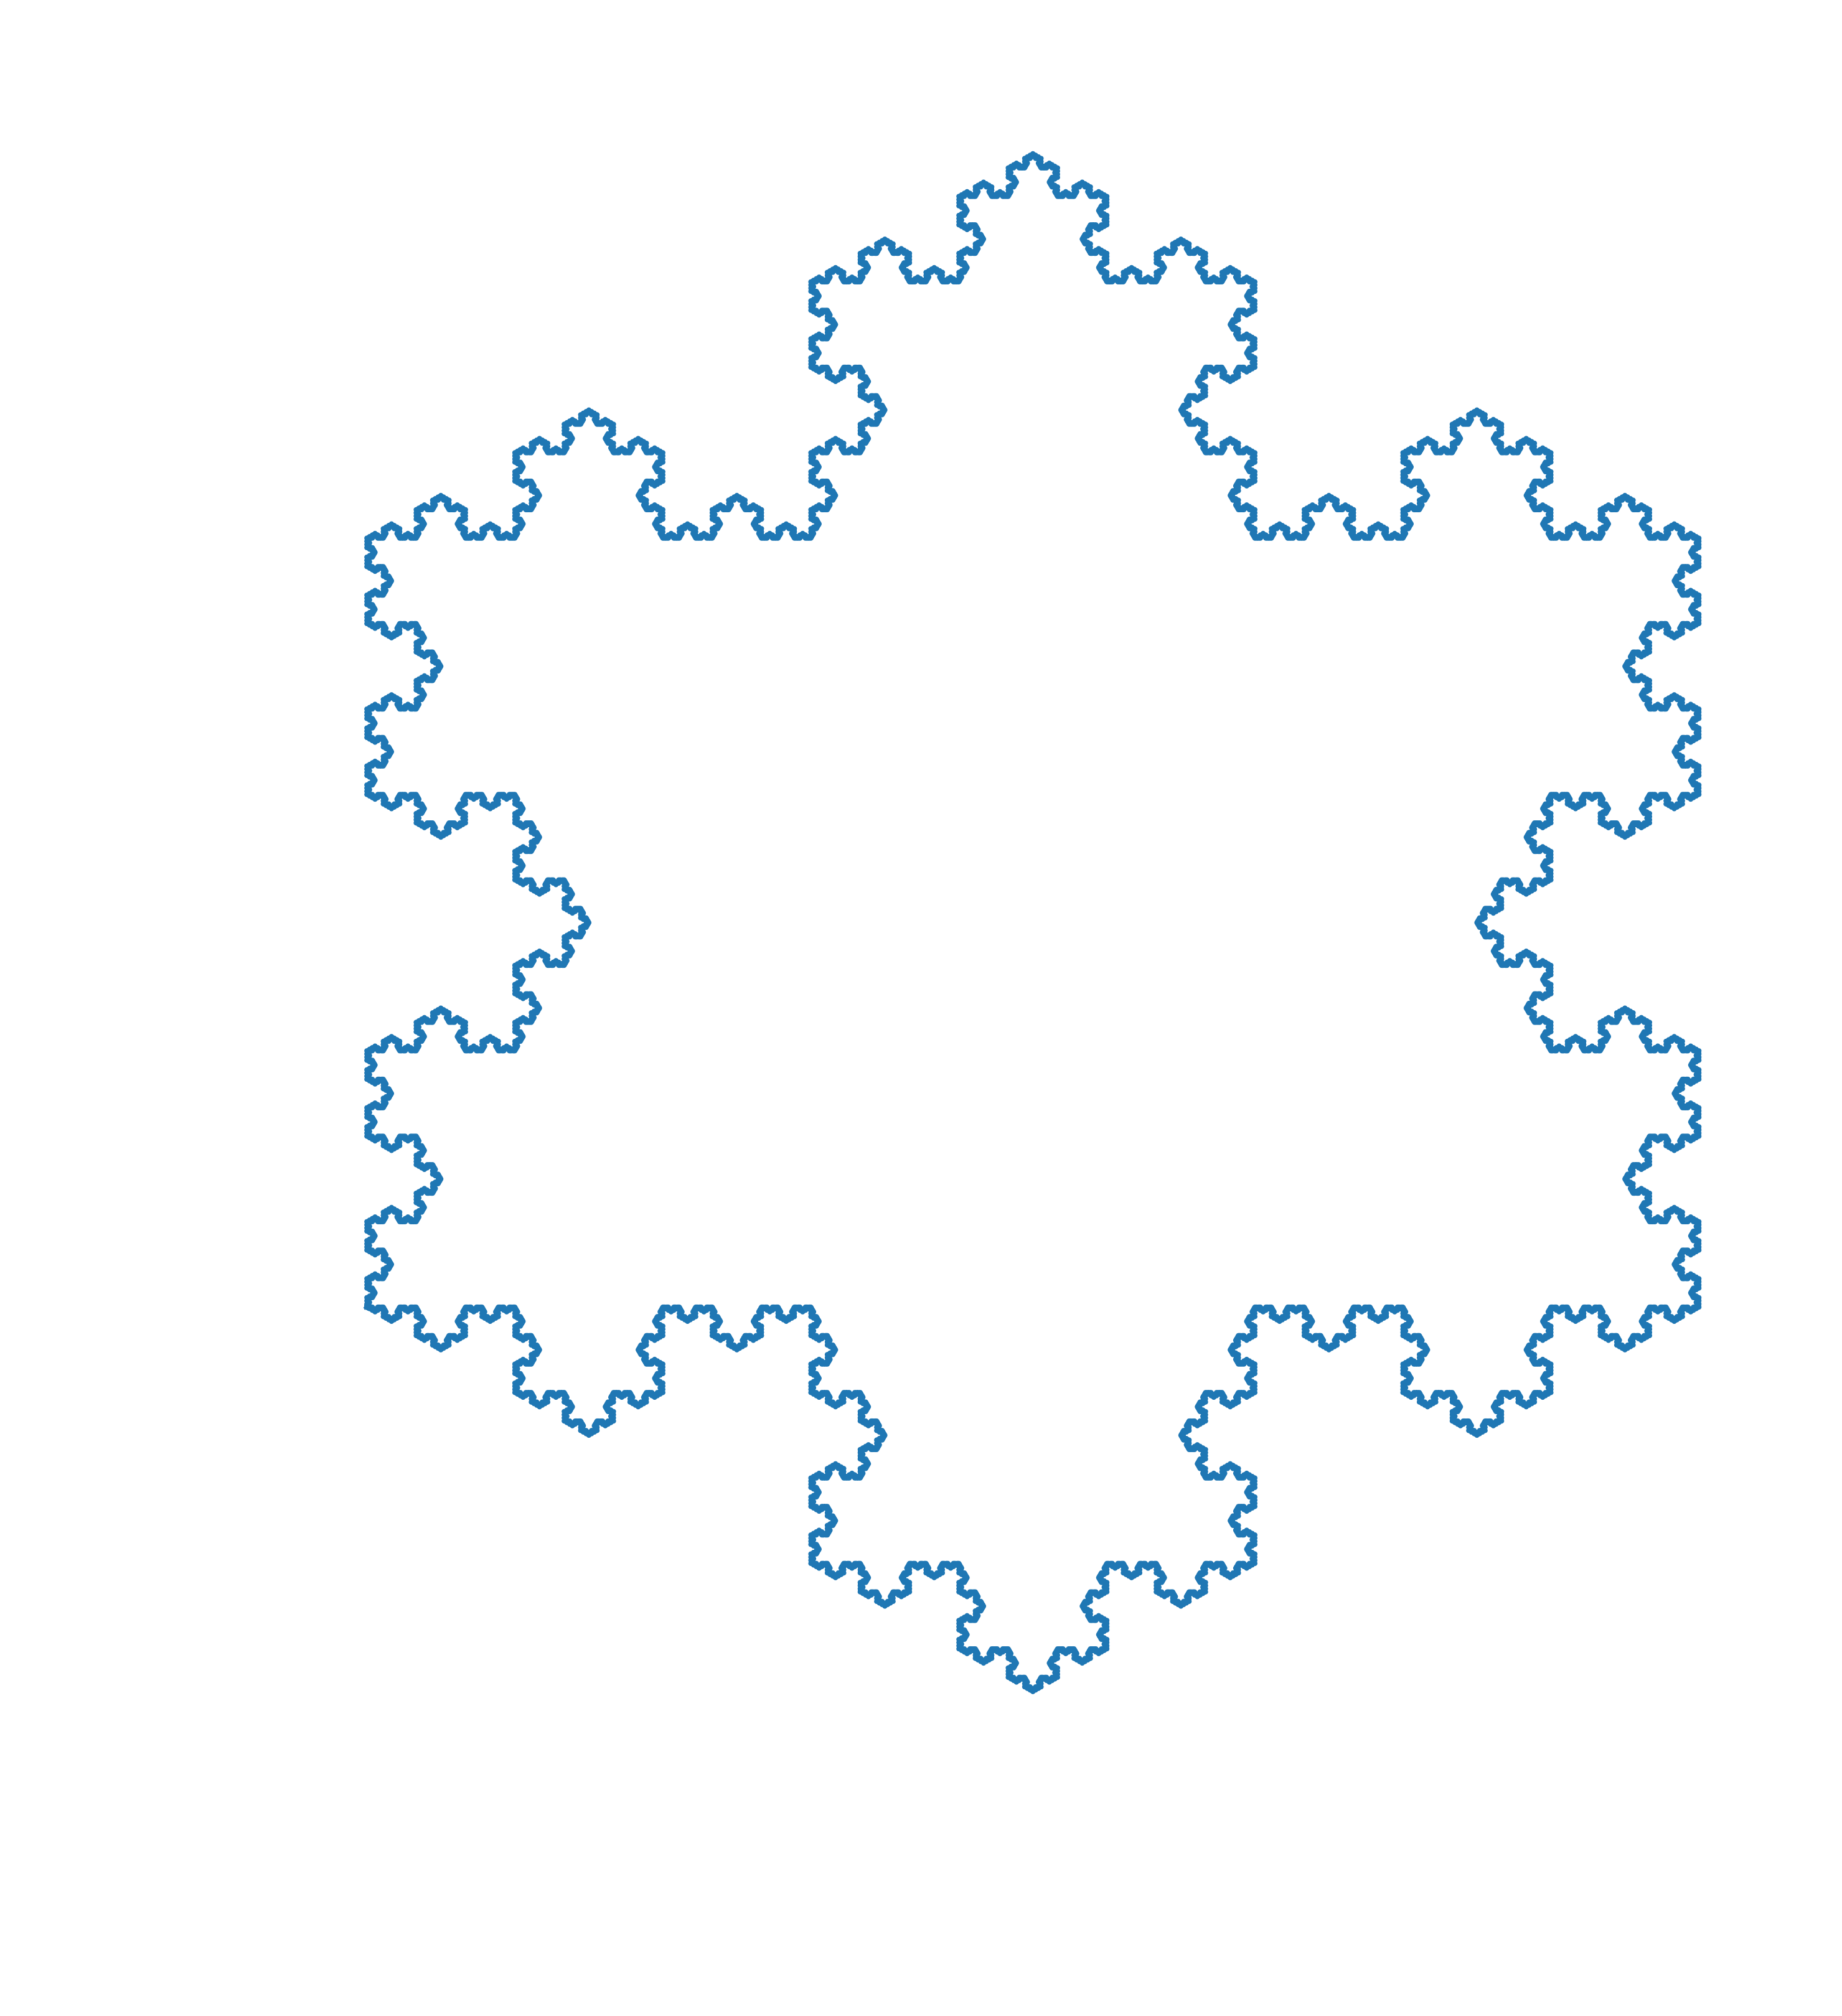
\includegraphics[width=.8\textwidth]{koch_6_it}
	\end{minipage}

	\vspace{1cm}
\end{frame}

\begin{frame}[t, c]{Koch snow flake}{A finite area within an infinite perimeter?}
	\centering
	\begin{minipage}{.48\textwidth}
		\begin{itemize}
			\item At the 7\textsuperscript{th} iteration:
			\begin{itemize}
				\item[$\hookrightarrow$] $N_7 = 3 \times 4^7$
				\item[$\hookrightarrow$] $S_7 = \nicefrac{1}{3^7}$
			\end{itemize}

			\bigskip

			\item We'll work out the area later.
		\end{itemize}
	\end{minipage}%
	\hfill
	\begin{minipage}{.48\textwidth}
		\centering
		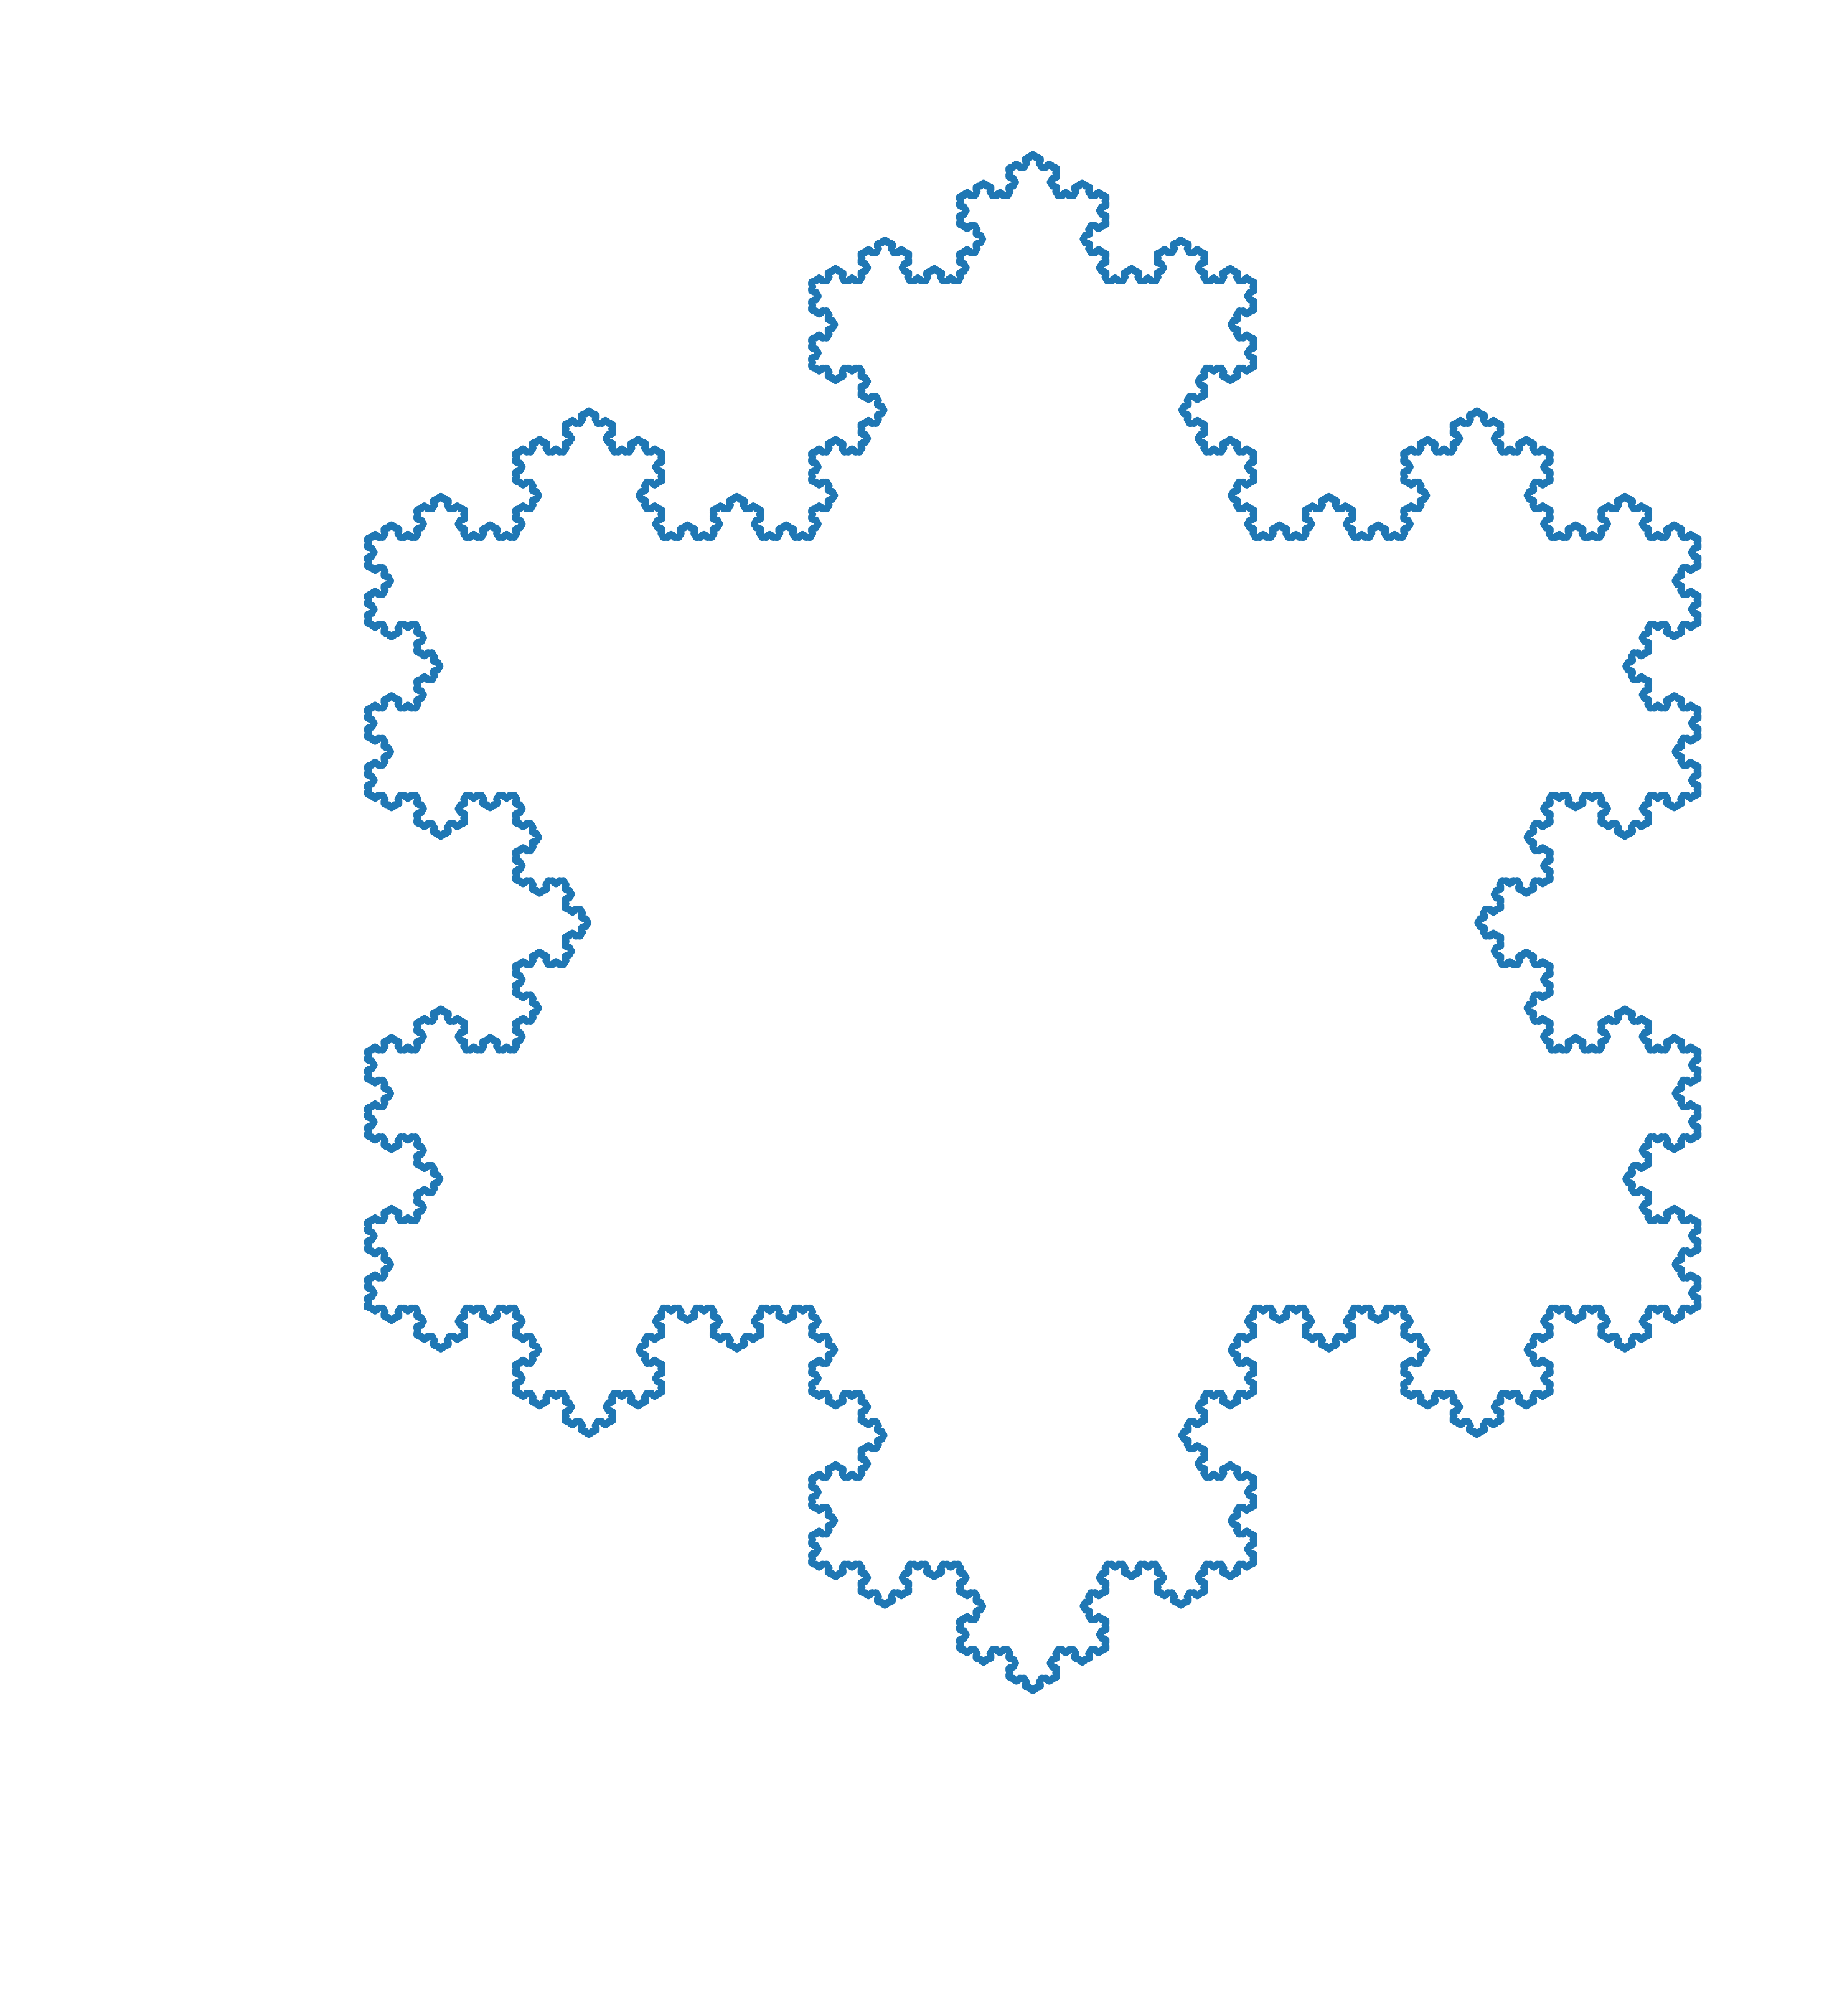
\includegraphics[width=.8\textwidth]{koch_7_it}
	\end{minipage}

	\vspace{1cm}
\end{frame}

\begin{frame}[t, c]{Koch snow flake}{A fnite area within an infinite perimeter?}
	\begin{itemize}
		\item The perimeter at the n\textsuperscript{th} iteration is given by
		$$
		P_n = N_n \times S_n = 3 \displaystyle \left( \frac{4}{3} \right)^n.
		$$
		\item Quite clearly, one has
		$$
		\lim_{n \to \infty} P_n = \infty,
		$$
		i.e.\ as $n \to \infty$, the perimeter of the curve goes to infinity.
	\end{itemize}

	\vspace{1cm}
\end{frame}

\begin{frame}[t, c]{Koch snow flake}{A finite area within an infinite perimeter?}
	\begin{itemize}
		\item The area at the n\textsuperscript{th} iteration is given by
		$$
		A_n = \displaystyle \frac{a_0}{5} \left( 8 - 3 \left( \frac{4}{9} \right)^n \right),
		$$
		with $a_0$ the area of the initial triangle.
		\medskip
		\item Quite clearly, one has
		$$
		\lim_{n \to \infty} A_n = \displaystyle \frac{8}{5} a_0.
		$$
		\item Suprisingly, the area remains finite despite the perimeter going to infinity...
	\end{itemize}

	\vspace{1cm}
\end{frame}

\begin{frame}[t, c]{How to define the dimension of a (self-similar) object?}{Disgression}
	\centering
	\Large{Au tableau.}

	\vspace{1cm}
\end{frame}

\begin{frame}[t, c]{Hausdorff dimension of well-known fractals}{Koch snowflake}
	\begin{minipage}{.48\textwidth}
		\centering
		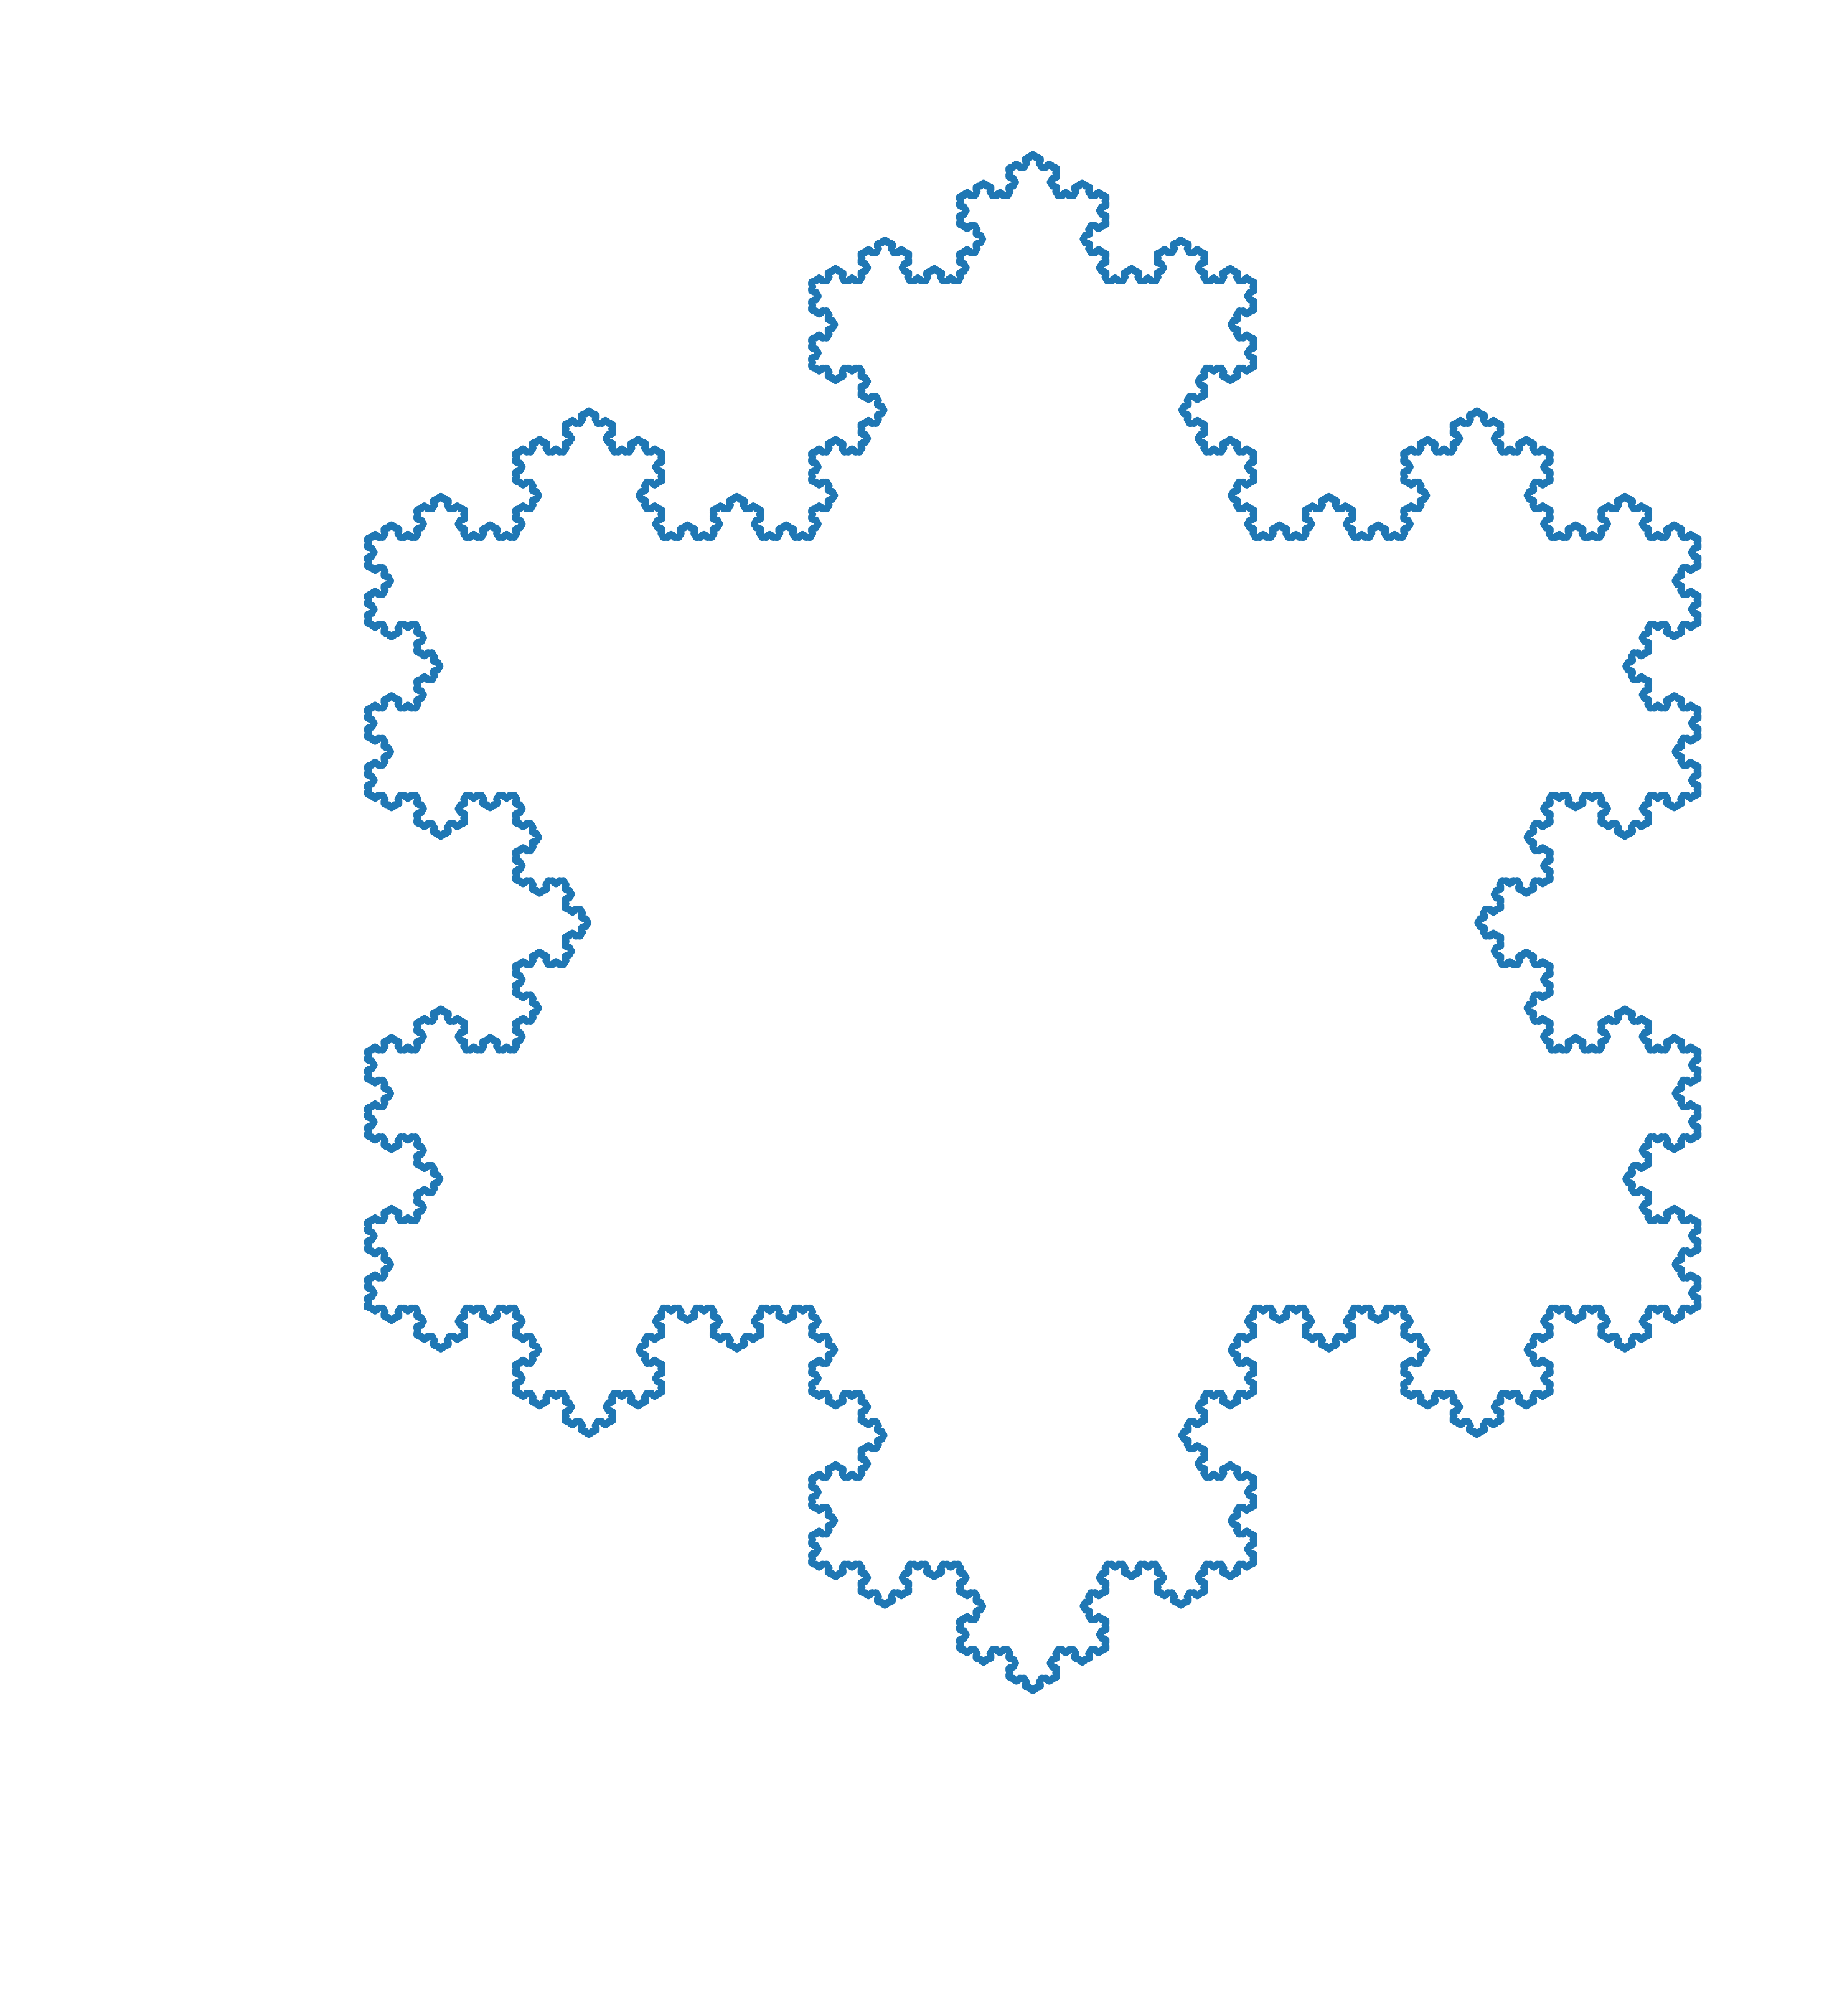
\includegraphics[width=.8\columnwidth]{koch_7_it}
	\end{minipage}%
	\hfill
	\begin{minipage}{.48\textwidth}
		\centering
		Hausdorff dimension
		$$
		\begin{aligned}
			D & = \displaystyle \frac{\ln(4)}{\ln(3)} \\
			& \simeq 1.2619
		\end{aligned}
		$$
	\end{minipage}
	\vspace{1cm}
\end{frame}

\begin{frame}[t, c]{Hausdorff dimension of well-known fractals}{Sierpinski triangle}
	\begin{minipage}{.48\textwidth}
		\centering
		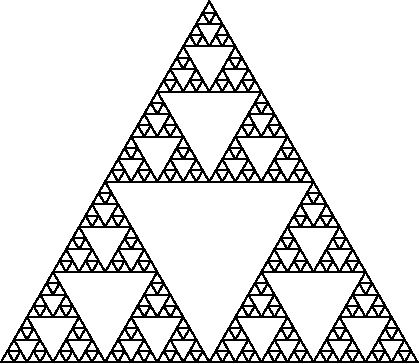
\includegraphics[width=.8\columnwidth]{sierpinski}
	\end{minipage}%
	\hfill
	\begin{minipage}{.48\textwidth}
		\centering
		Hausdorff dimension
		$$
		\begin{aligned}
			D & = \displaystyle \frac{\ln(3)}{\ln(2)} \\
			& \simeq 1.5849
		\end{aligned}
		$$
	\end{minipage}

	\vspace{1cm}
\end{frame}

\begin{frame}[t, c]{Hausdorff dimension of well-known fractals}{Feigenbaum tree}
	\begin{minipage}{.48\textwidth}
		\centering
		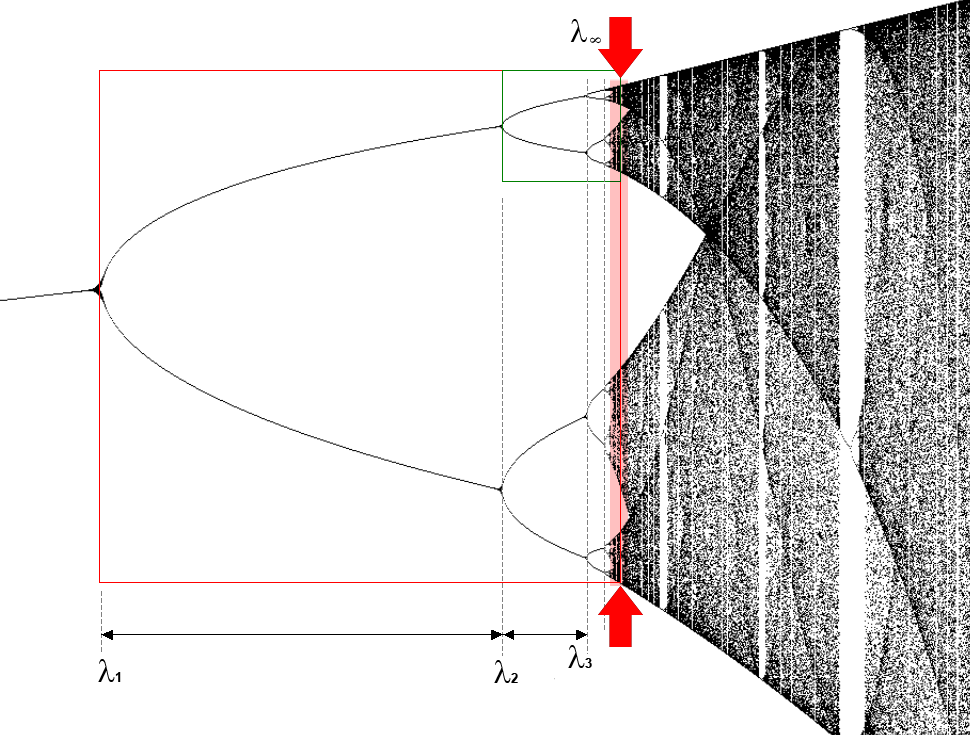
\includegraphics[width=.8\columnwidth]{Feigenbaum_attractor}
	\end{minipage}%
	\hfill
	\begin{minipage}{.48\textwidth}
		\centering
		Hausdorff dimension
		$$
		D \simeq 0.538
		$$
	\end{minipage}

	\vspace{1cm}
\end{frame}

\begin{frame}[t, c]{Hausdorff dimension of well-known fractals}{R\"ossler attractor}
	\begin{minipage}{.48\textwidth}
		\centering
		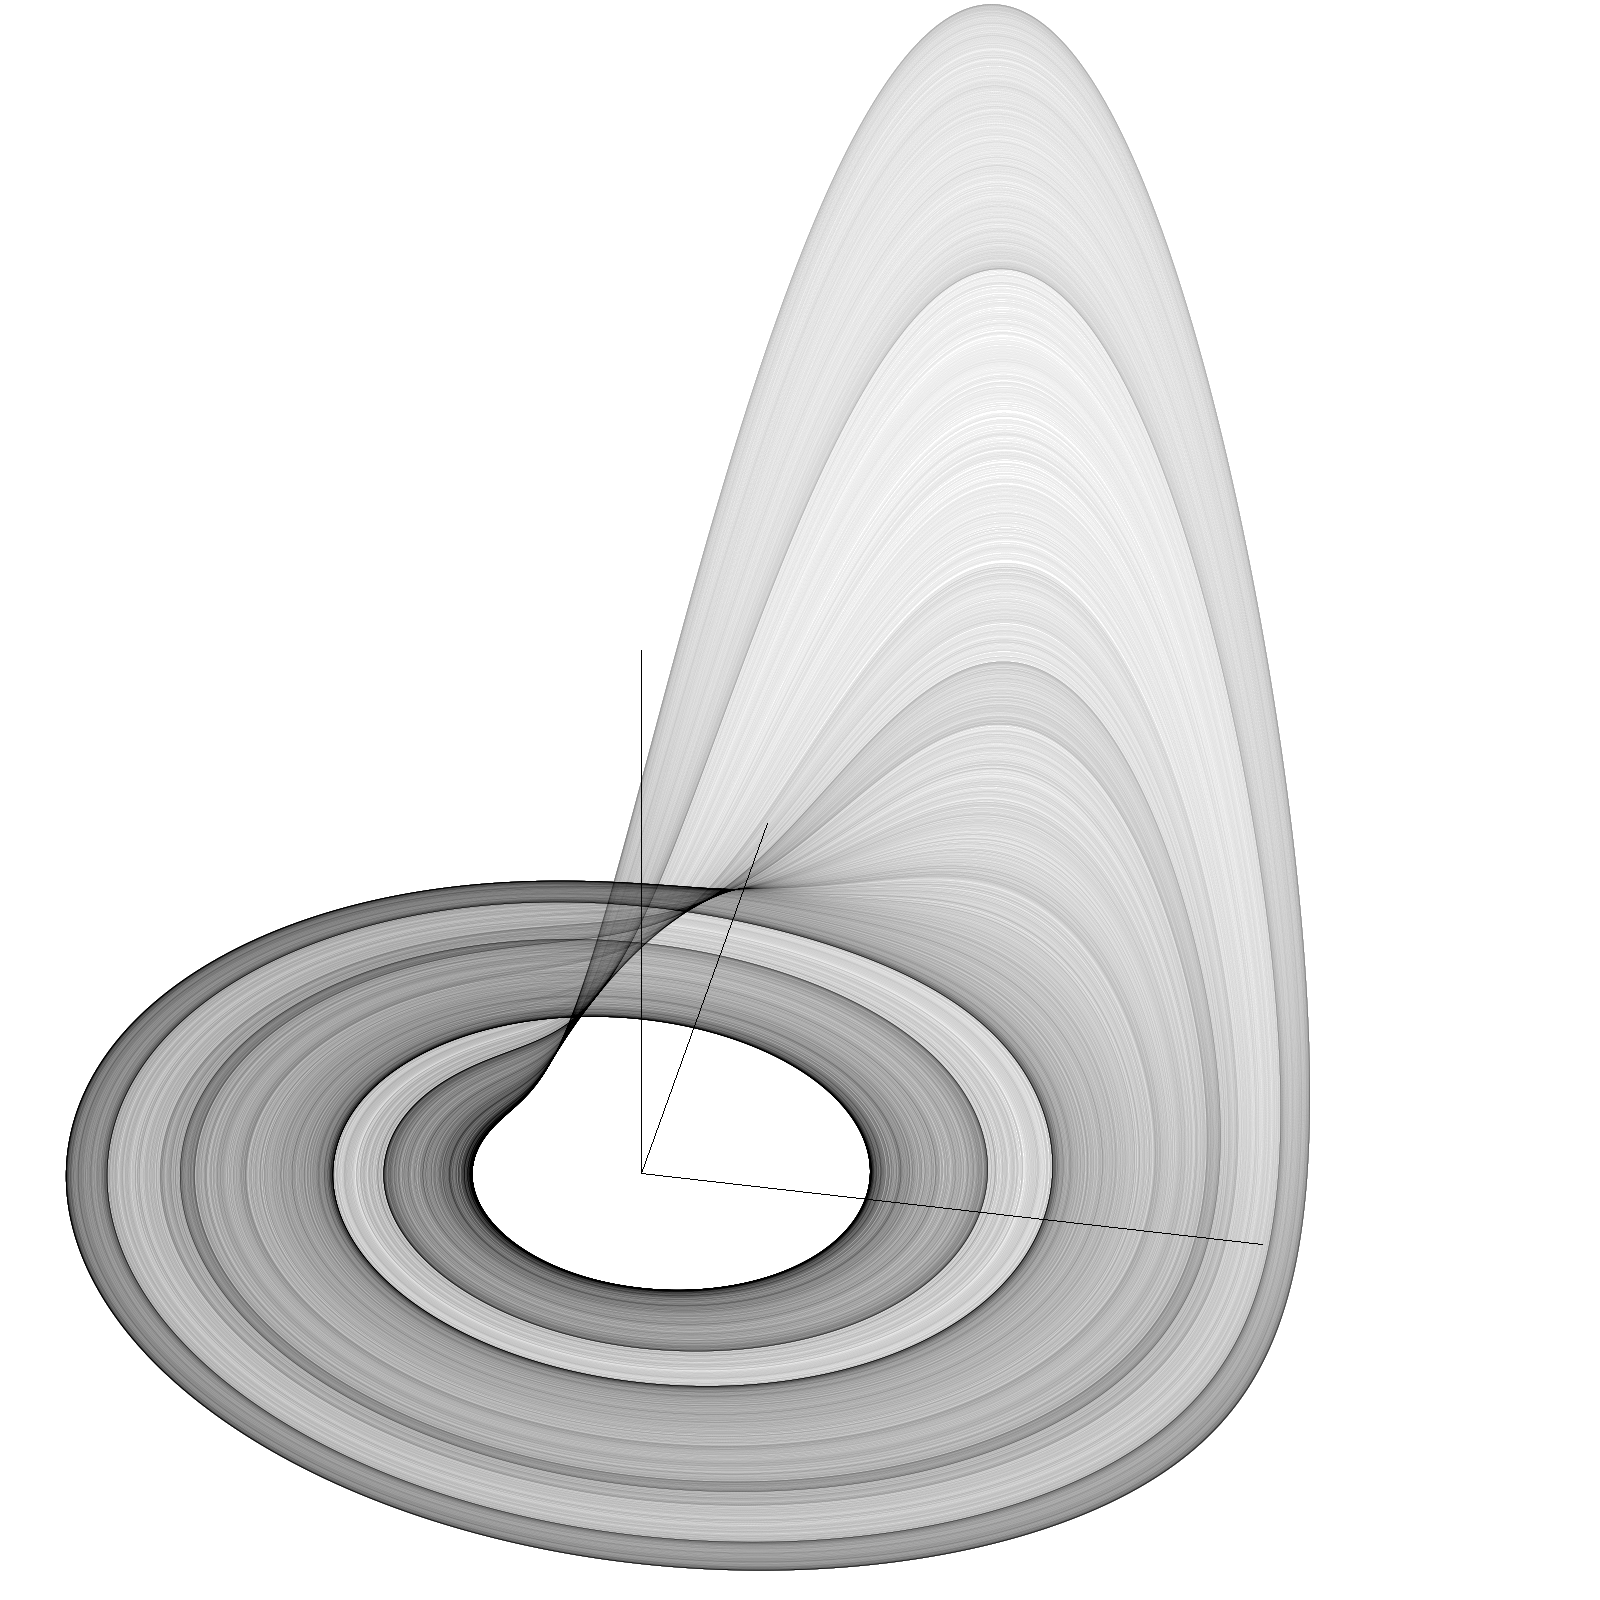
\includegraphics[width=.8\columnwidth]{Roessler_attractor}
	\end{minipage}%
	\hfill
	\begin{minipage}{.48\textwidth}
		\centering
		Hausdorff dimension
		$$
		D \simeq 2.01 \pm 0.01
		$$
	\end{minipage}

	\vspace{1cm}
\end{frame}

\begin{frame}[t, c]{Hausdorff dimension of well-known fractals}{Lorenz attractor}
	\begin{minipage}{.48\textwidth}
		\centering
		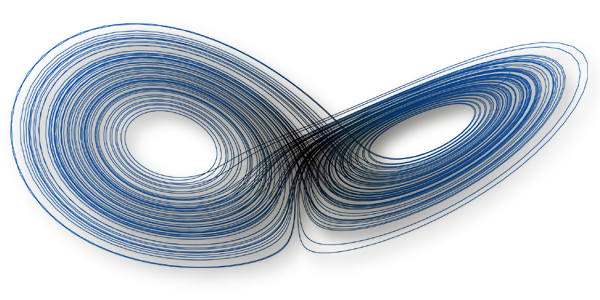
\includegraphics[width=.8\columnwidth]{cover}
	\end{minipage}%
	\hfill
	\begin{minipage}{.48\textwidth}
		\centering
		Hausdorff dimension
		$$
		D \simeq 2.06 \pm 0.01
		$$
	\end{minipage}

	\vspace{1cm}
\end{frame}


%-------------------------------------------------------------------------------
%                           MANDELBROT AND JULA SETS
%-------------------------------------------------------------------------------


\begin{frame}[t, c]{}
	\centering
	\vspace{1cm}

	{\Large \textbf{Mandelbrot and Julia sets}}

	\bigskip

	{\textgre{\textbf{Beautiful computer visualizations}}}

\end{frame}

\begin{frame}[t, c]{Julia sets}{Preliminaries}
	\begin{itemize}
		\item Named after \emph{Gaston Julia} and \emph{Pierre Fatou}, French mathematicians from the early 20\textsuperscript{th} century.
		\medskip
		\item Consider a function
		$$
		f(x) = \displaystyle \frac{P(x)}{Q(x)}
		$$
		with $P$ and $Q$ two polynomials without common divisors.
		\medskip
		\item The filled-in Julia set $J_f$ is the set of points $x \in \mathbb{C}$ for which
		$$
		\left\{
		\begin{aligned}
			& z_0 = x \\
			\lim_{n \to \infty} & z_{n+1} = f(z_n) < \infty.
		\end{aligned}
		\right.
		$$
		\begin{itemize}
			\item[$\hookrightarrow$] The true Julia set $J$ is the boundry of the filled-in set.
		\end{itemize}
	\end{itemize}
	\vspace{1cm}
\end{frame}

\begin{frame}[t, c]{Julia sets}{Preliminaries}
	\begin{minipage}{.48\textwidth}
		\begin{itemize}
			\item Let us consider
			$$f(z) = z^2 - 1.$$

			\medskip

			\item The corresponding filled-in Julia set is a \emph{connected set}.
			\begin{itemize}
				\item[$\hookrightarrow$] Also called the \emph{Fatou set} of $f(z)$.
			\end{itemize}
		\end{itemize}
	\end{minipage}%
	\hfill
	\begin{minipage}{.48\textwidth}
		\centering
		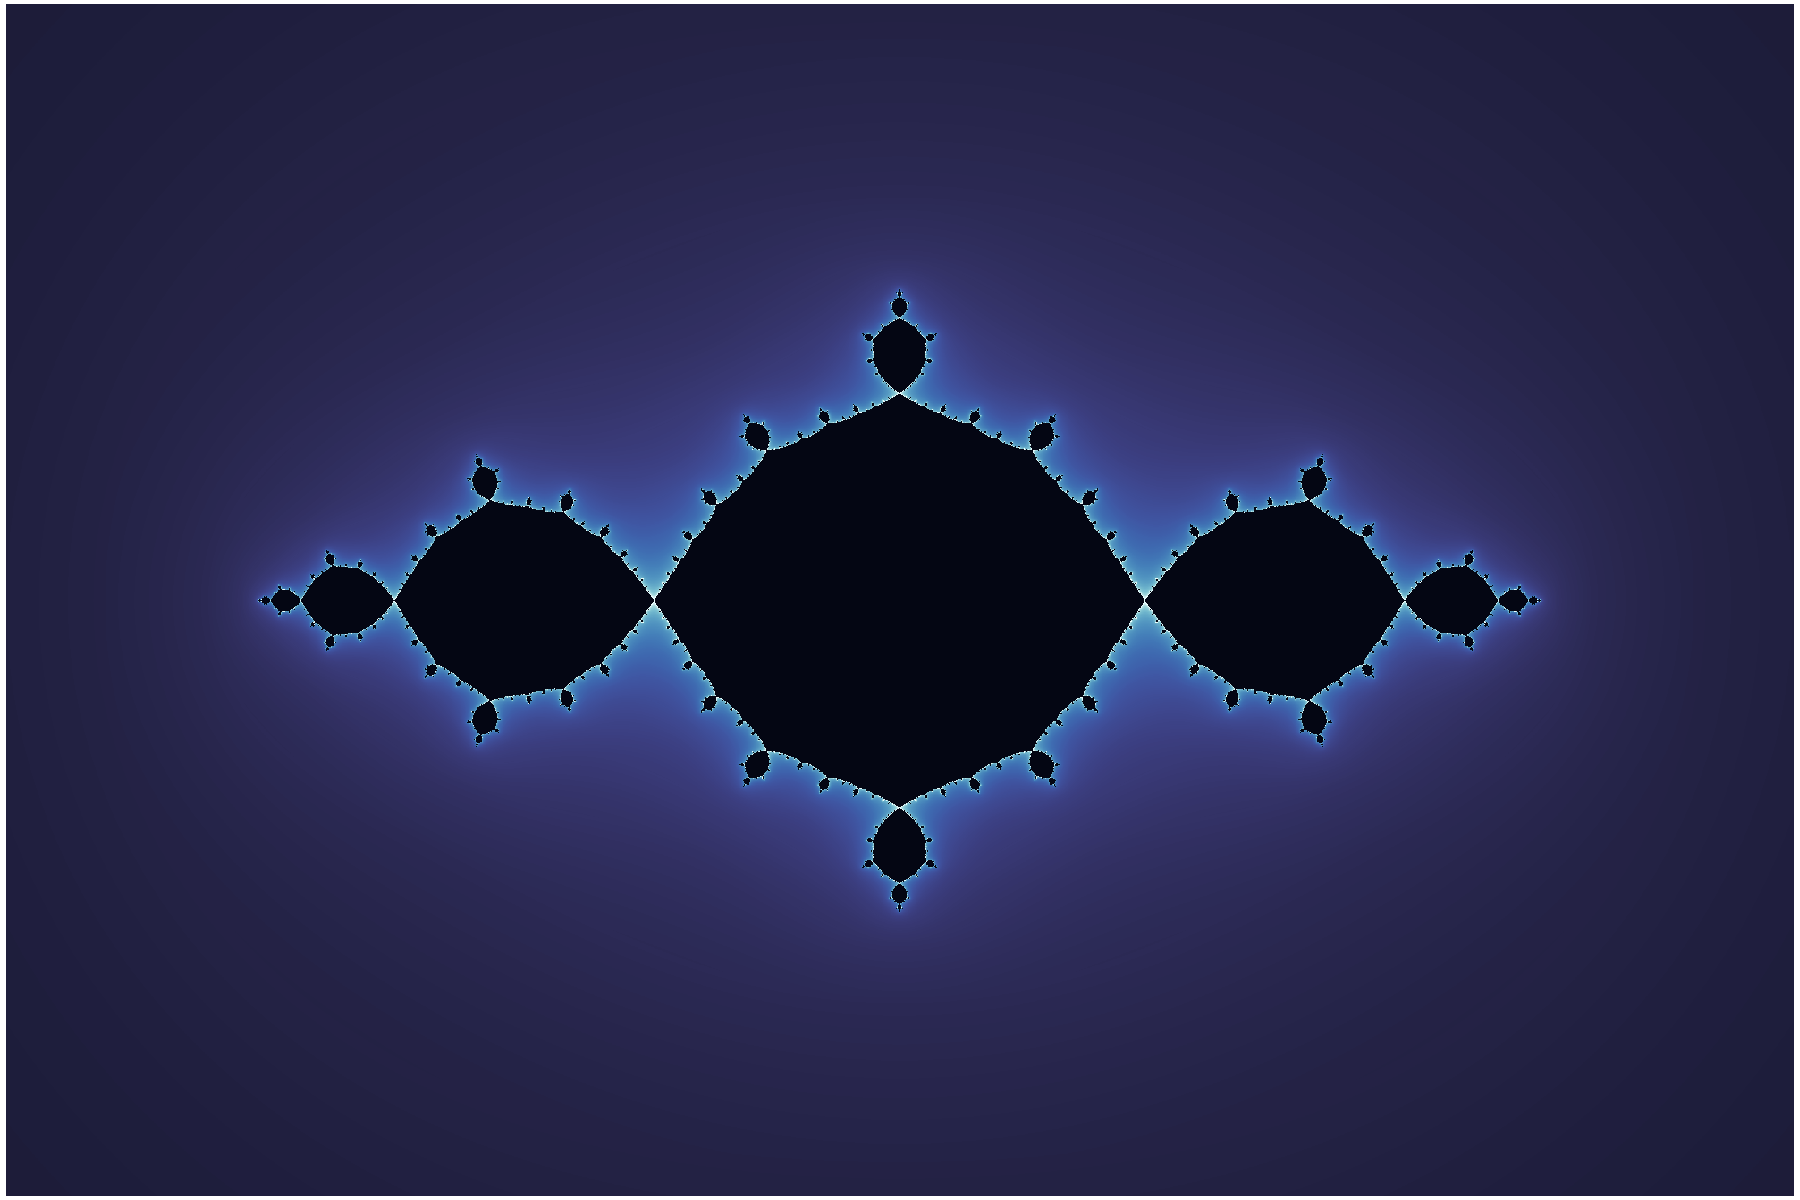
\includegraphics[width=\columnwidth]{Julia_set_1} \\
		\medskip
		Julia set for $c = -1$.
	\end{minipage}

	\vspace{1cm}
\end{frame}

\begin{frame}[t, c]{Julia sets}{Preliminaries}
	\begin{minipage}{.48\textwidth}
		\centering
		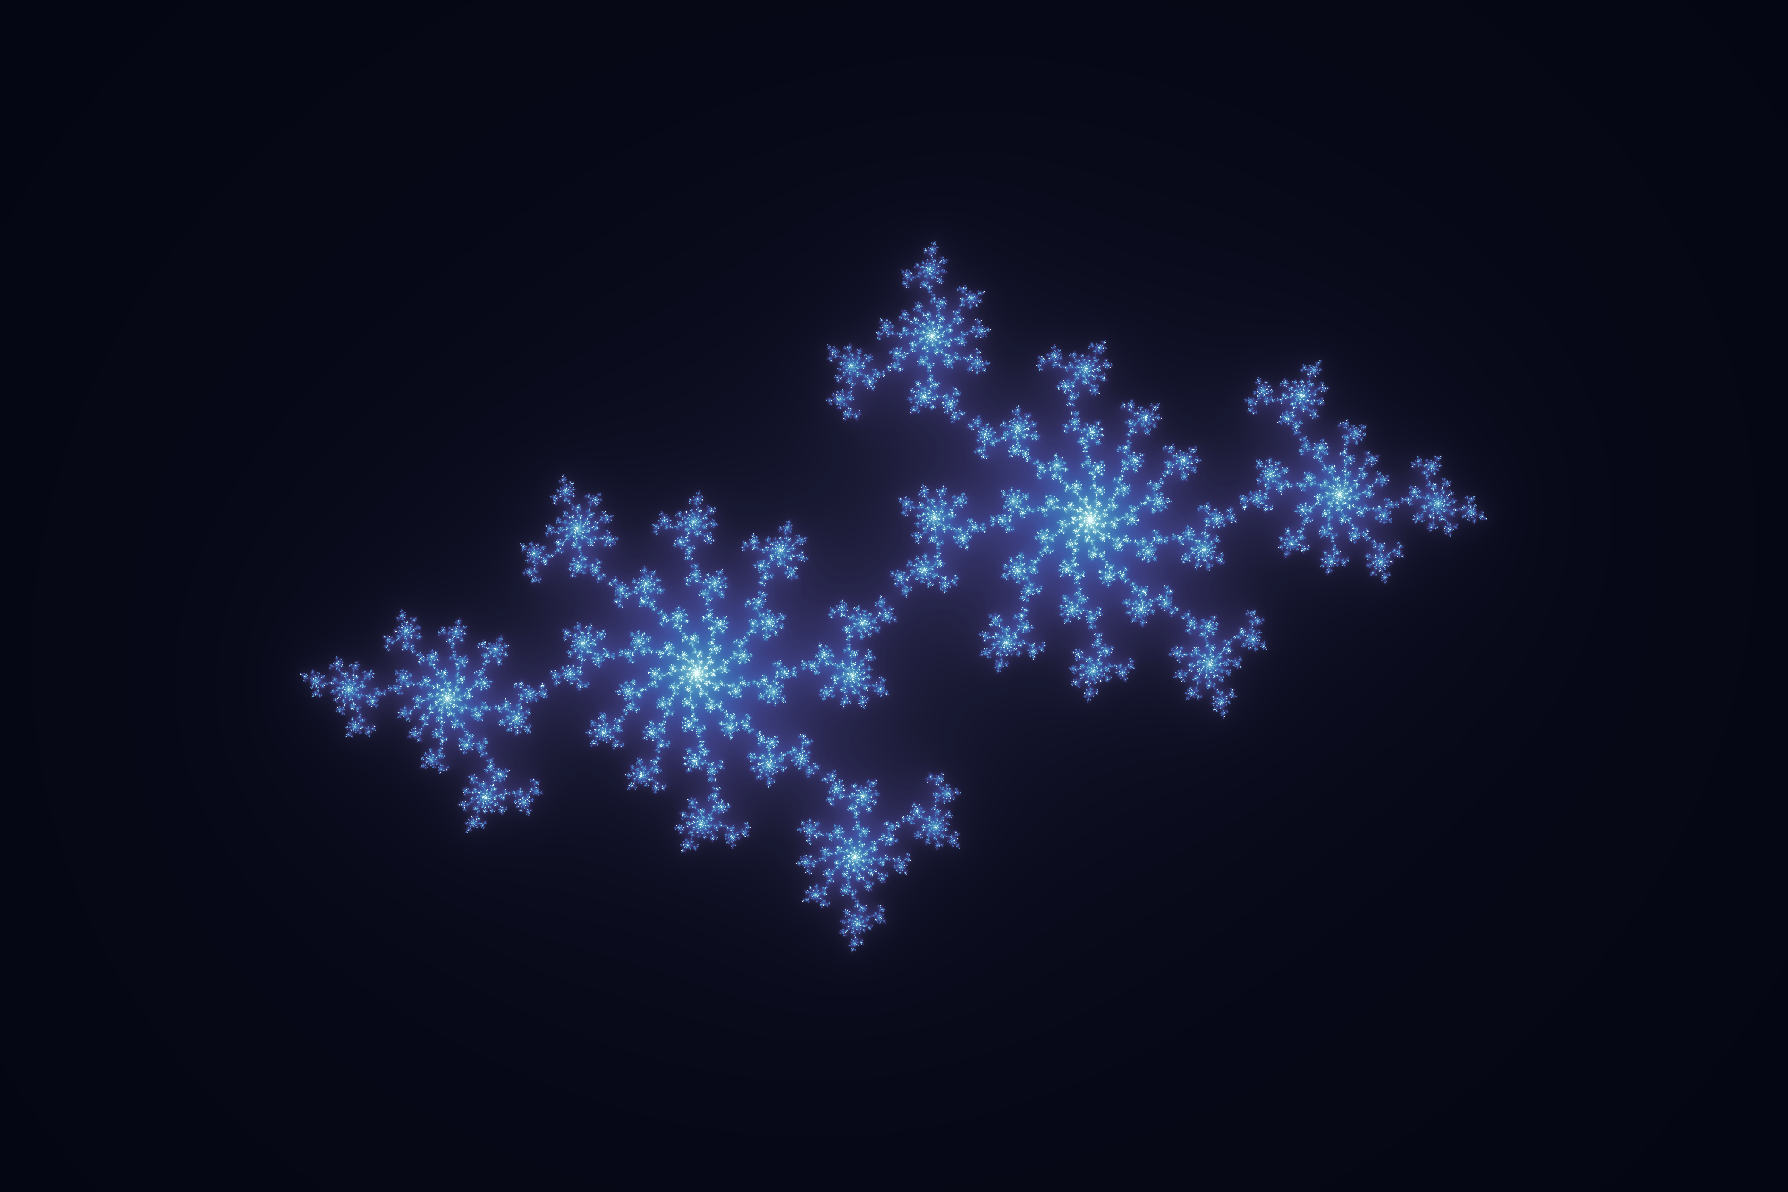
\includegraphics[width=\columnwidth]{Julia_set_2} \\
		\medskip
		Julia set for $c = - 0.70176 - i0.3842$.
	\end{minipage}%
	\hfill
	\begin{minipage}{.48\textwidth}
		\begin{itemize}
		\item Let us consider
		$$f(z) = z^2 - (0.7016 - i0.3842).$$

		\medskip

		\item The corresponding Julia set is a \emph{disconnected set}.
		\begin{itemize}
			\item[$\hookrightarrow$] Also called the \emph{Cantor set} of $f(z)$.
			\item[$\hookrightarrow$] Sometime called \emph{Fatou dust}.
		\end{itemize}
	\end{itemize}
	\end{minipage}

	\vspace{1cm}
\end{frame}

\begin{frame}[t, c]{Julia sets}{Preliminaries}
	\centering
	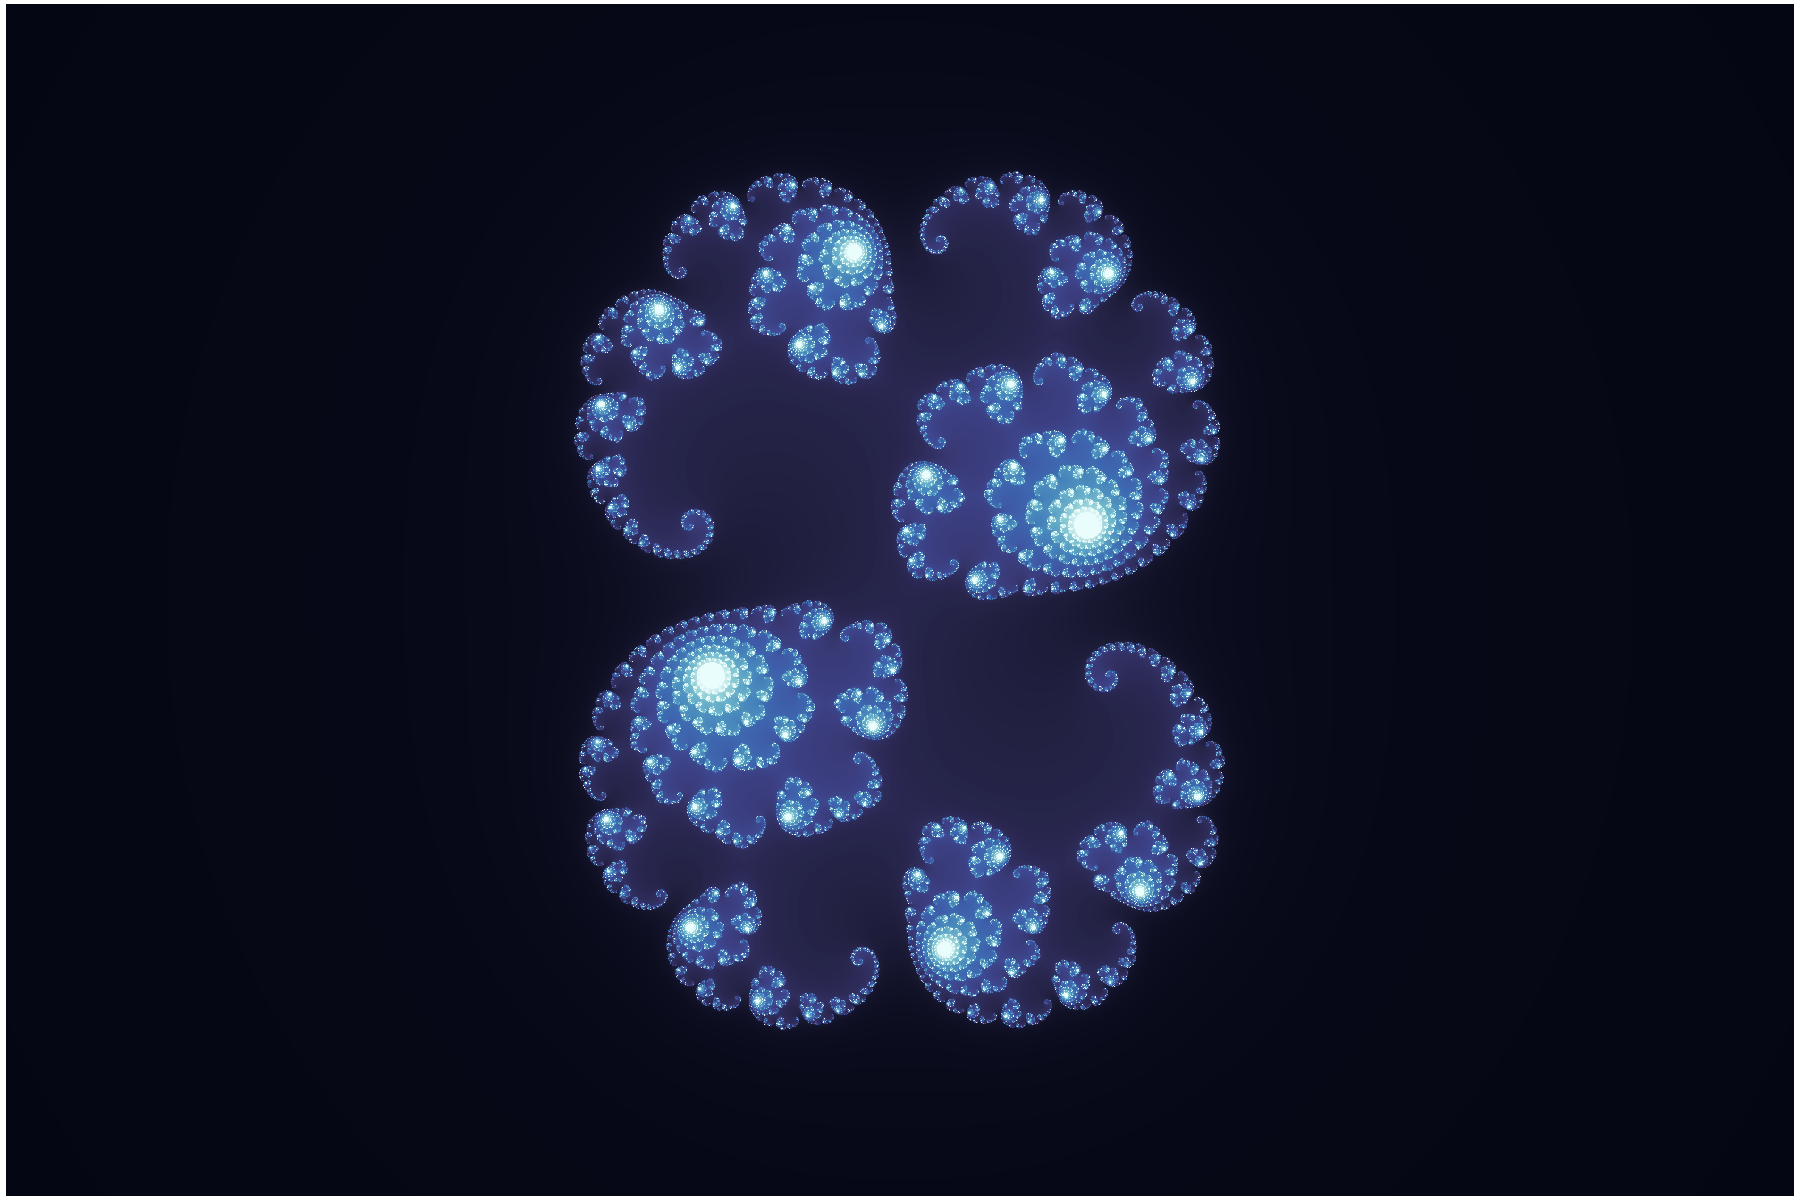
\includegraphics[width=.6\textwidth]{Julia_set_3} \\
	\medskip
	Julia set for $c = 0.285 + i0.01$.

	\vspace{1cm}
\end{frame}

\begin{frame}[t, c]{Julia sets}{Preliminaries}
	\centering
	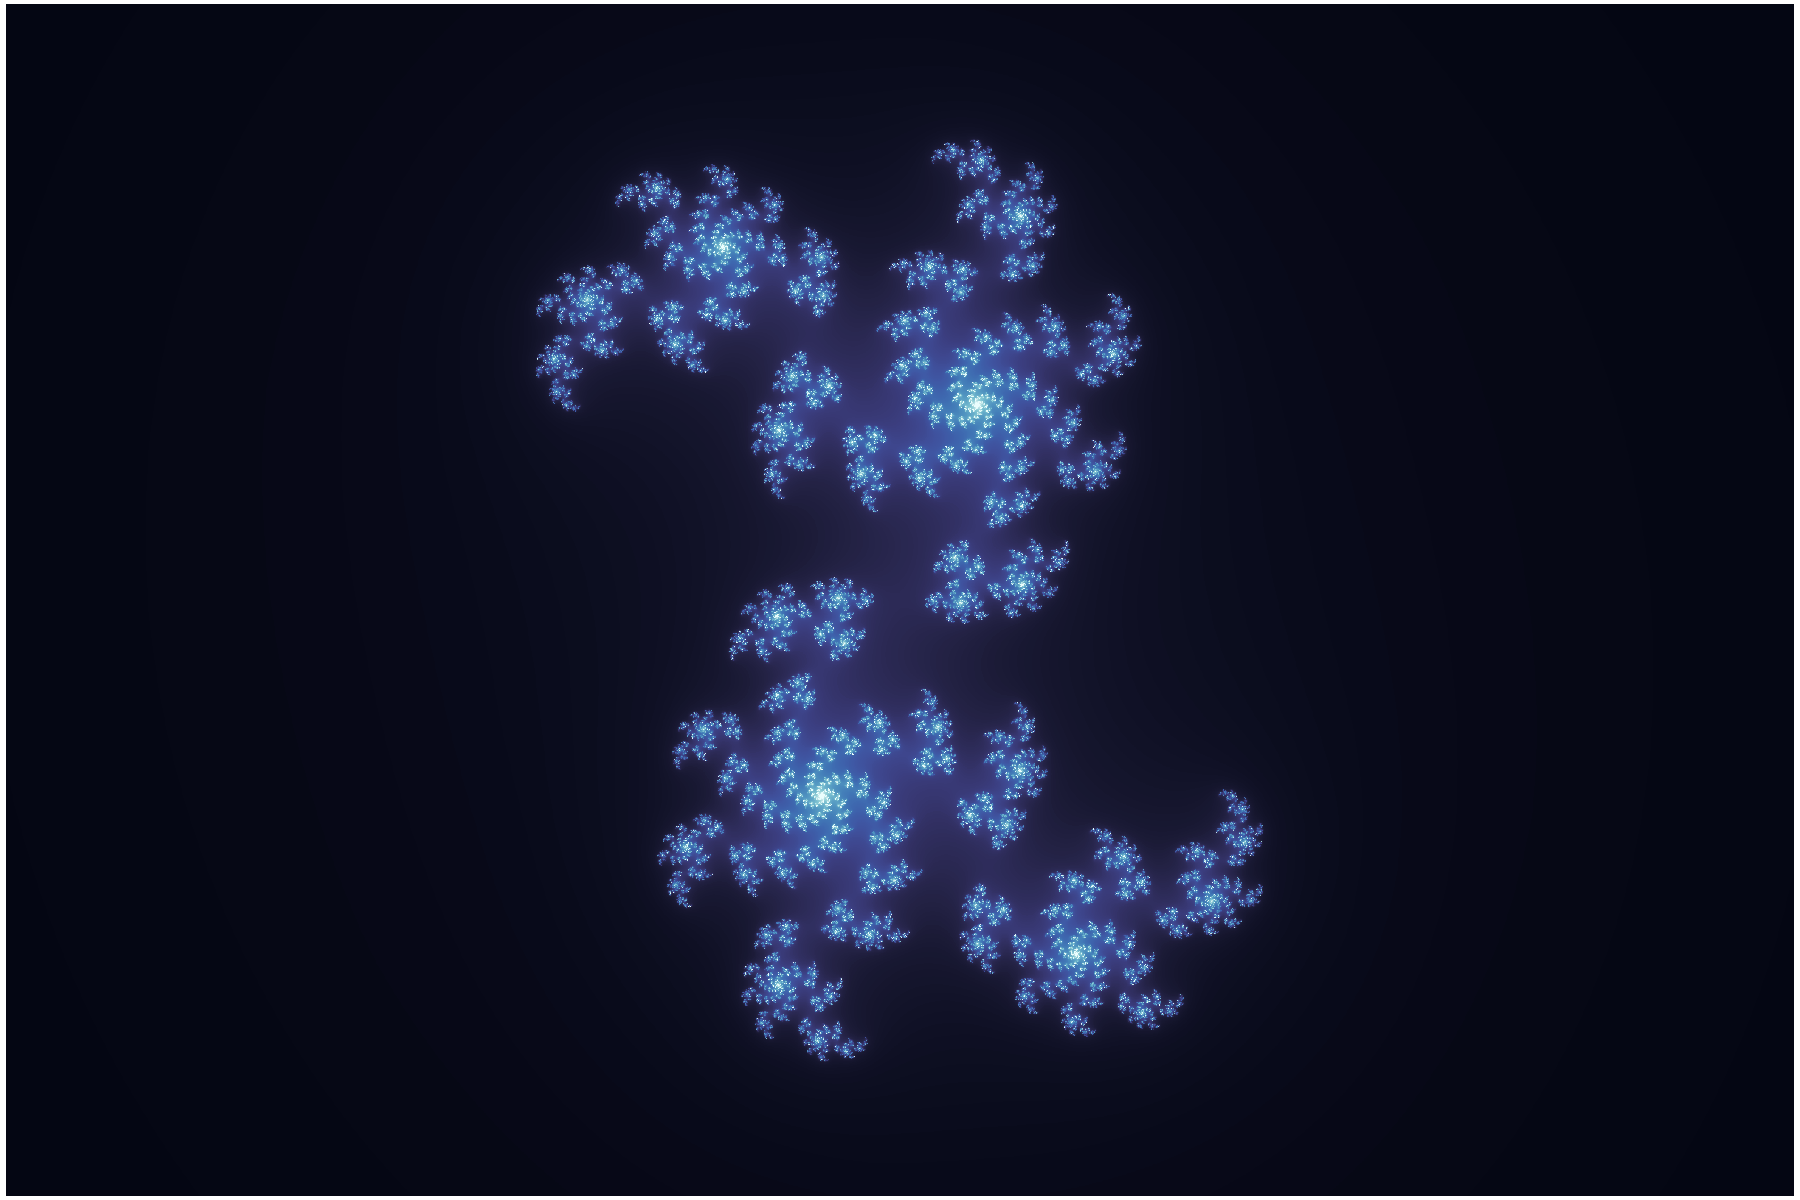
\includegraphics[width=.6\textwidth]{Julia_set_4} \\
	\medskip
	Julia set for $c = 0.4 + i0.3$.
	\vspace{1cm}
\end{frame}

\begin{frame}[t, c]{Julia sets}{Preliminaries}
	\centering
	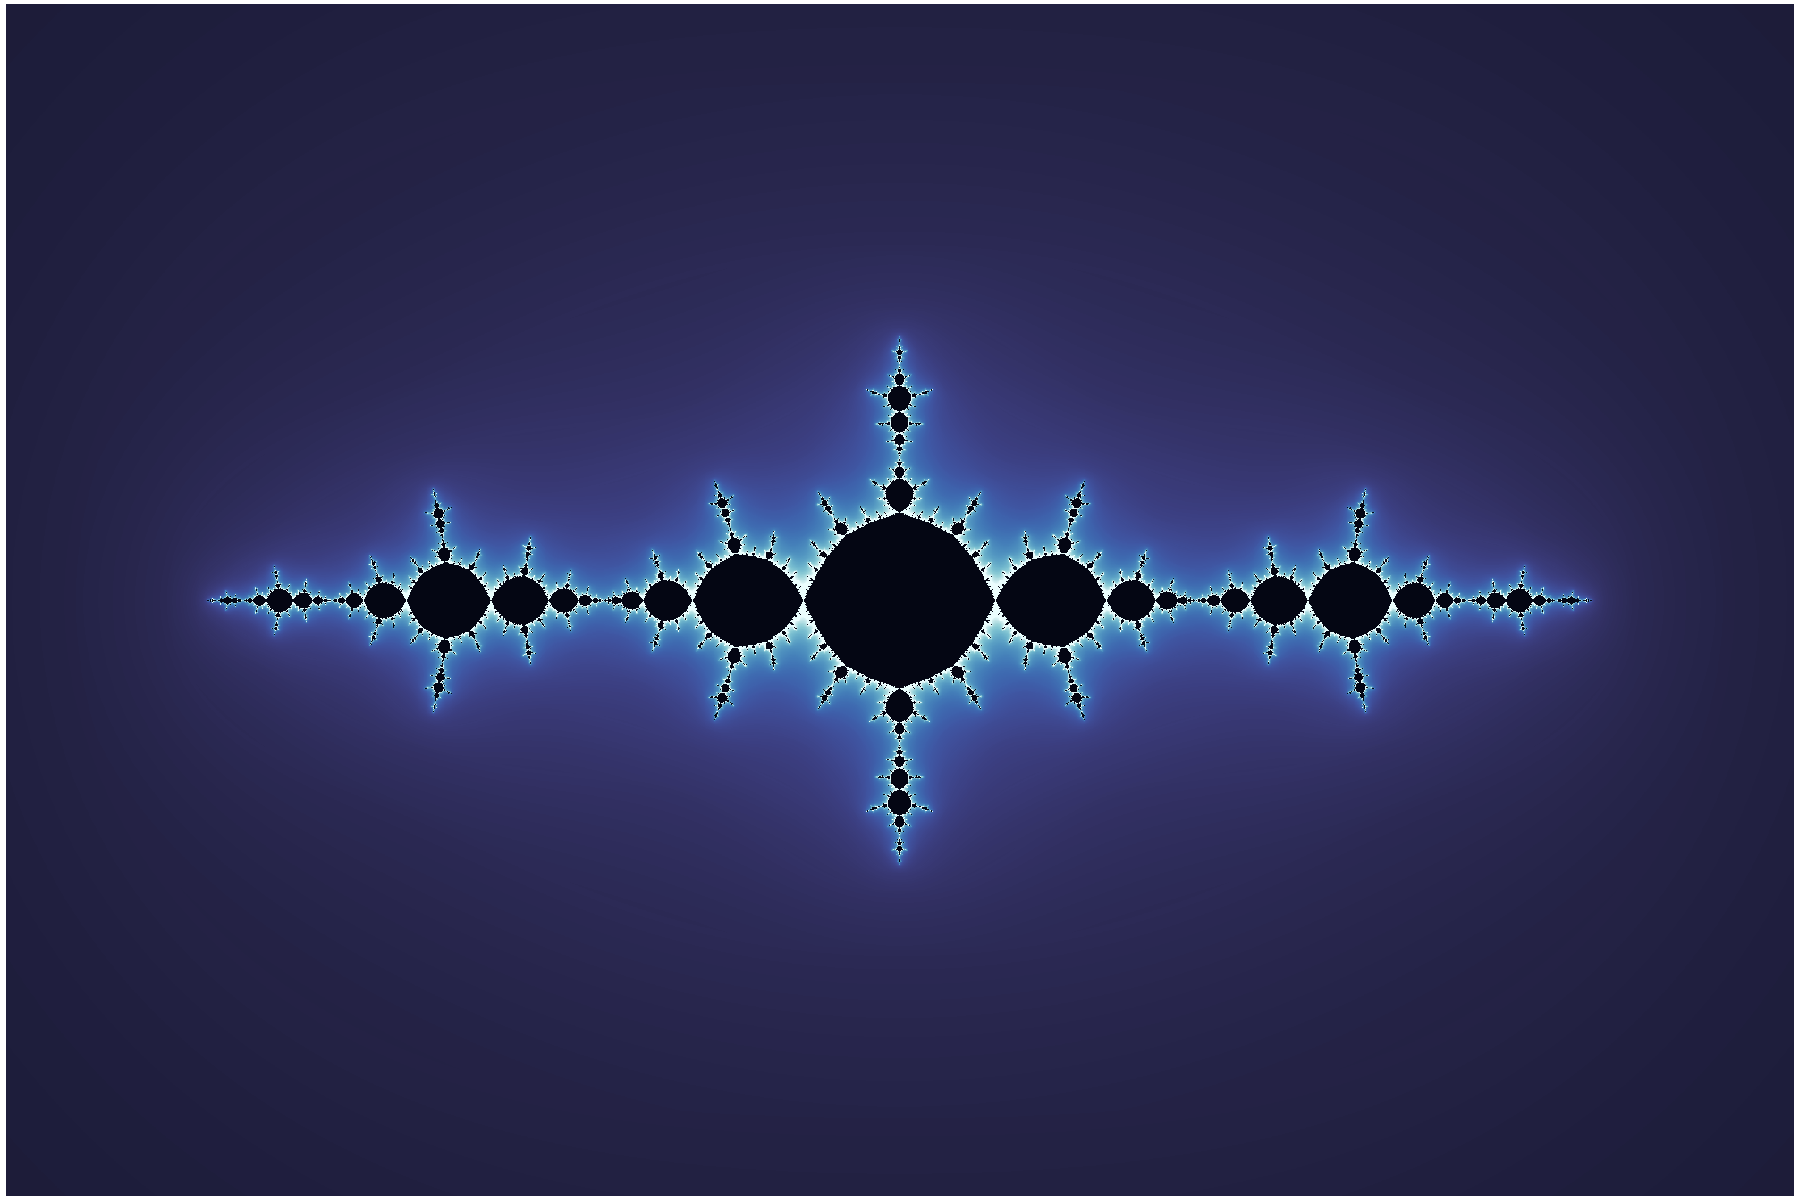
\includegraphics[width=.6\textwidth]{Julia_set_5} \\
	\medskip
	Julia set for $c = -1.3$.
	\vspace{1cm}
\end{frame}

\begin{frame}[t, c]{Julia sets}{Question}
	\centering
	\begin{block}{\centering \textbf{Question}}
		\centering
		Can we predict if, for a given $c$, the corresponding Julia set will be connected or not?
	\end{block}
	\vspace{1cm}
\end{frame}

\begin{frame}[t, c]{Julia sets}{Fundamental Dichotomy Theorem}
	\centering
	\begin{block}{\centering \textbf{Theorem}}
		If the orbit of $0$ under the iteration $z^2 + c$ escapes to infinity, the Julia set $J_c$ is topologically the same as the Cantor set (i.e.\ disconnected). Otherwise, $J_c$ is a connected Fatou set.
	\end{block}

	\bigskip

	\begin{block}{\centering \textbf{Proof}}
		\centering
		Beyond the scope of the present course.
	\end{block}

	\vspace{1cm}
\end{frame}

\begin{frame}[t, c]{Mandelbrot set}{Definition}
	\begin{itemize}
		\item Given $f_c = x^2 + c$, the Mandelbrot set $\mathcal{M}$ is defined as
		$$
		\mathcal{M} = \left\{ c \in \mathbb{C} : J(f_c) \text{ is connected.}\right\}
		$$
		\medskip
		\item Alternatively, we can define it as the set of points $c \in \mathbb{C}$ such that the iteration
		\begin{equation}
			\left\{
			\begin{aligned}
				& z_0 = 0 \\
				& z_{n+1} = z_n^2 + c
			\end{aligned}
			\right.
			\notag
		\end{equation}
		is bounded as $n \to \infty$.
	\end{itemize}

	\vspace{1cm}
\end{frame}

\begin{frame}[t, c]{Mandelbrot set}{$\mathcal{M}$ is included in the closed disk of radius 2}
	\begin{block}{\centering \textbf{Demonstration} }
		\centering
		Proove that the Mandelbrot set $\mathcal{M}$ is included in the closed disk of radius 2.
	\end{block}

	\bigskip

	\underline{\textbf{Hint}}: Show by induction that when $z_0 = 0$ and $z_{n+1} = z_n^2 + c$, with $\vert c \vert = 2 + \epsilon$ (for $\epsilon > 0$), that
	$$
	\vert z_n \vert \geq 2 + (2^n - 1) \epsilon
	$$
	for all integer $n>0$.

	\vspace{1cm}
\end{frame}

\begin{frame}[t, c]{Mandelbrot set}{The set of connected Julia sets}
	\begin{minipage}{.48\textwidth}
		\begin{itemize}
			\item It is one of the most incredible mathematical object ever discovered by mankind.
			\medskip
			\item All of its secrets have not been unveiled yet.
			\begin{itemize}
				\item[$\hookrightarrow$] Fibonacci sequence and $\pi$ are both embeded within the M-set.
			\end{itemize}
			\medskip
			\item You can find numerous zoom-in animations on Youtube.
		\end{itemize}
	\end{minipage}%
	\hfill
	\begin{minipage}{.48\textwidth}
		\centering
		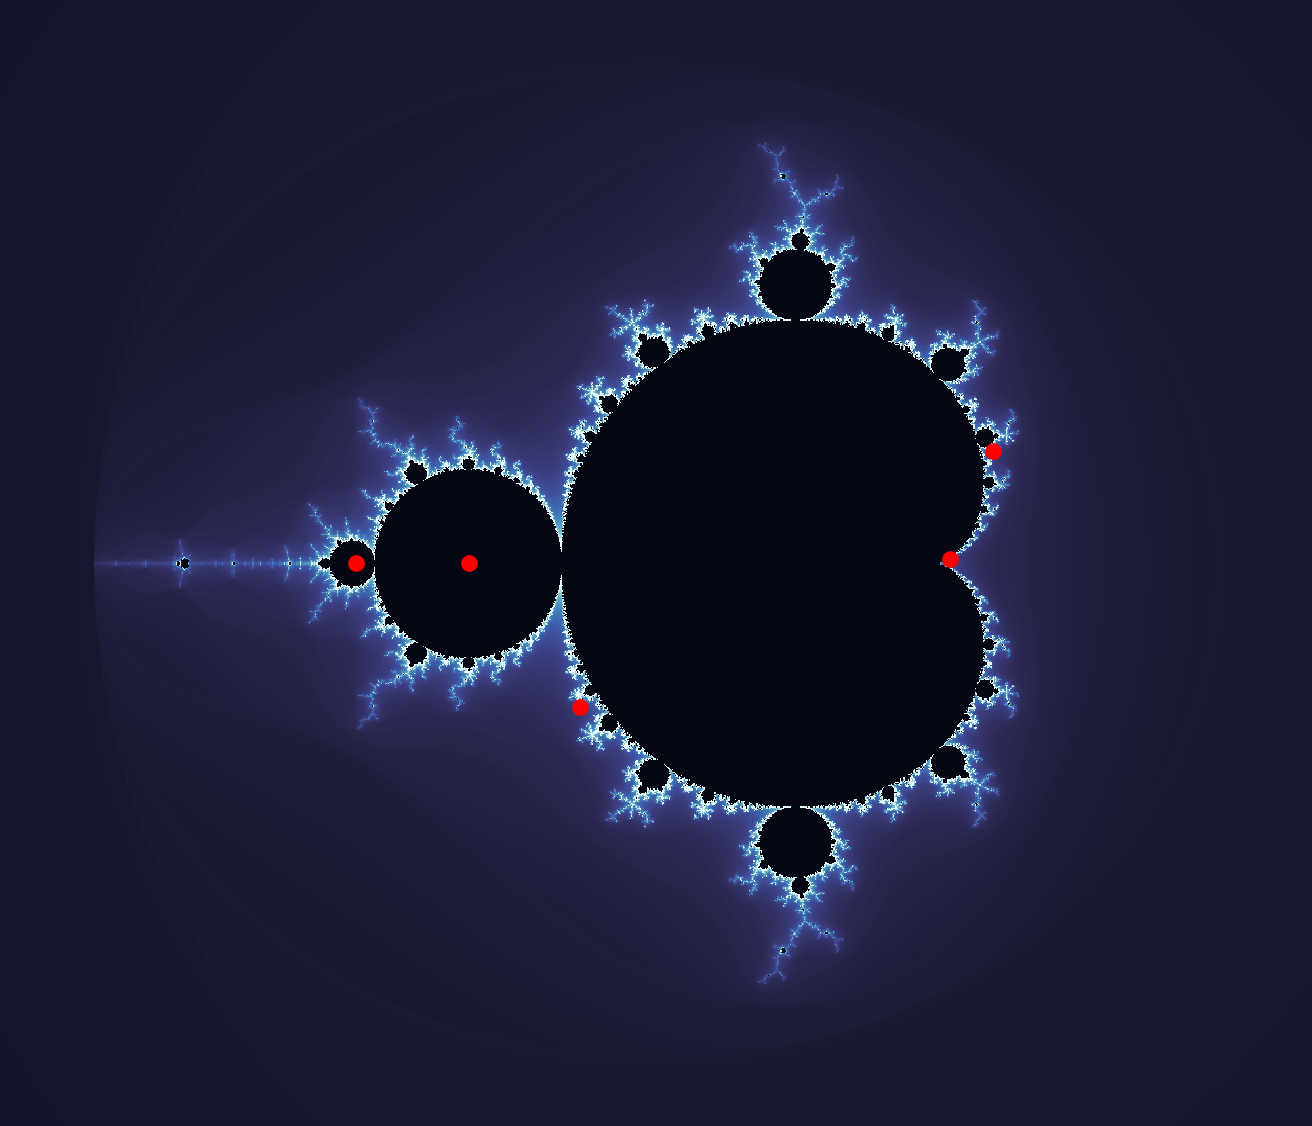
\includegraphics[width=\columnwidth]{Mandelbrot_set_bis}
	\end{minipage}

	\vspace{1cm}
\end{frame}


%-------------------------------------------------------------------------------
%                           ON THE CONNECTION BETWEEN M.S AND L.E
%-------------------------------------------------------------------------------


\begin{frame}[t, c]{}
	\centering
	\vspace{1cm}

	{\Large \textbf{Mandelbrot set and the Logistic equation}}

	\bigskip

	{\textgre{\textbf{A surprising connection}}}

\end{frame}

\begin{frame}[t, c]{Mandelbrot set}{Recap.}

	\begin{minipage}{.48\textwidth}
		\centering
		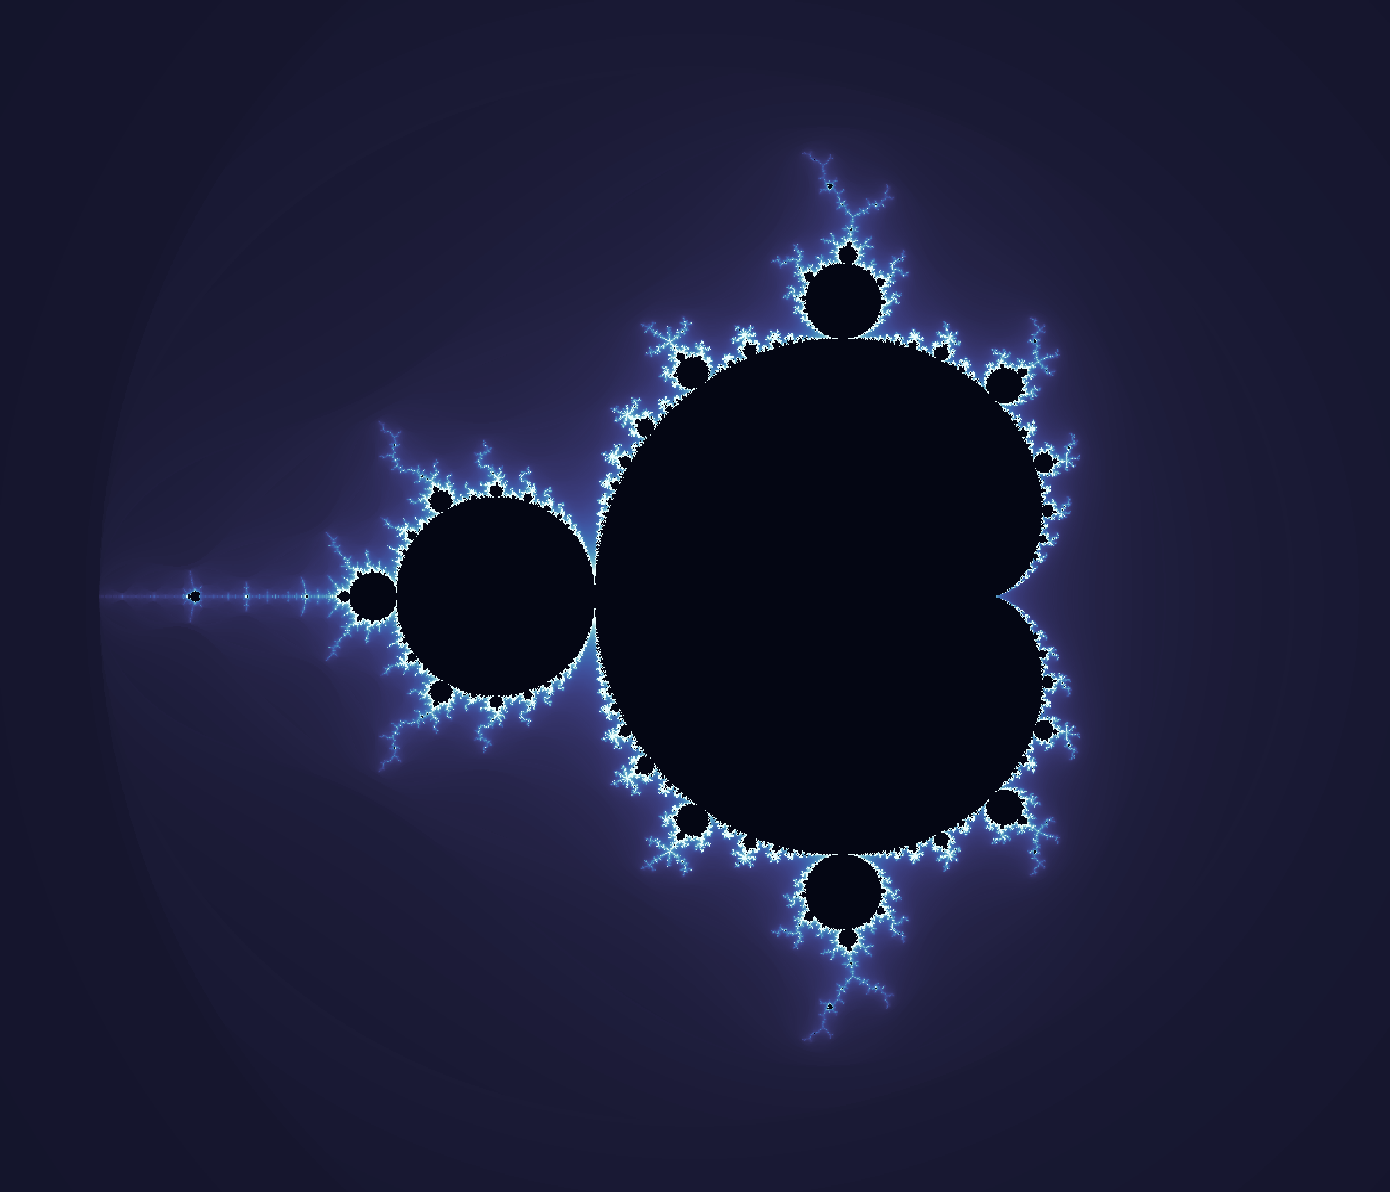
\includegraphics[width=\columnwidth]{Mandelbrot_set}
	\end{minipage}%
	\hfill
	\begin{minipage}{.48\textwidth}
		\begin{itemize}
			\item It is the set of points $c \in \mathbb{C}$ such that the iteration
			\begin{equation}
				\left\{
				\begin{aligned}
					& z_0 = 0 \\
					& z_{n+1} = z_n^2 + c
				\end{aligned}
				\right.
				\notag
			\end{equation}
			is bounded as $n \to \infty$.
		\end{itemize}
	\end{minipage}
	\vspace{1cm}
\end{frame}

\begin{frame}[t, c]{Logistic equation}{Recap.}
	\begin{minipage}{.48\textwidth}
		\begin{itemize}
			\item It is given by
			$$ x_{k+1} = \mu x_k \left( 1 - x_k \right).$$

			\item We have already studied it in Lecture 1, Lecture 5 and Lecture 7.

			\medskip

			\item Transition to chaos is through the \emph{subharmonic cascade}.
		\end{itemize}
	\end{minipage}%
	\hfill
	\begin{minipage}{.48\textwidth}
		\centering
		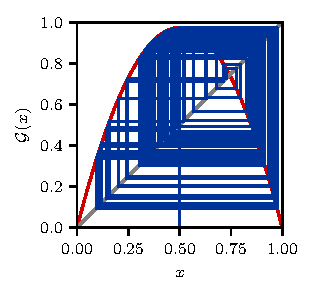
\includegraphics[width=.75\columnwidth]{logistic_map_cobweb_plot_9}\\
		Cobweb plot for the logistic map in a chaotic regime.
	\end{minipage}

	\vspace{1cm}
\end{frame}

\begin{frame}[t, c]{Logistic equation}{Bifurcation diagram}
	\centering
	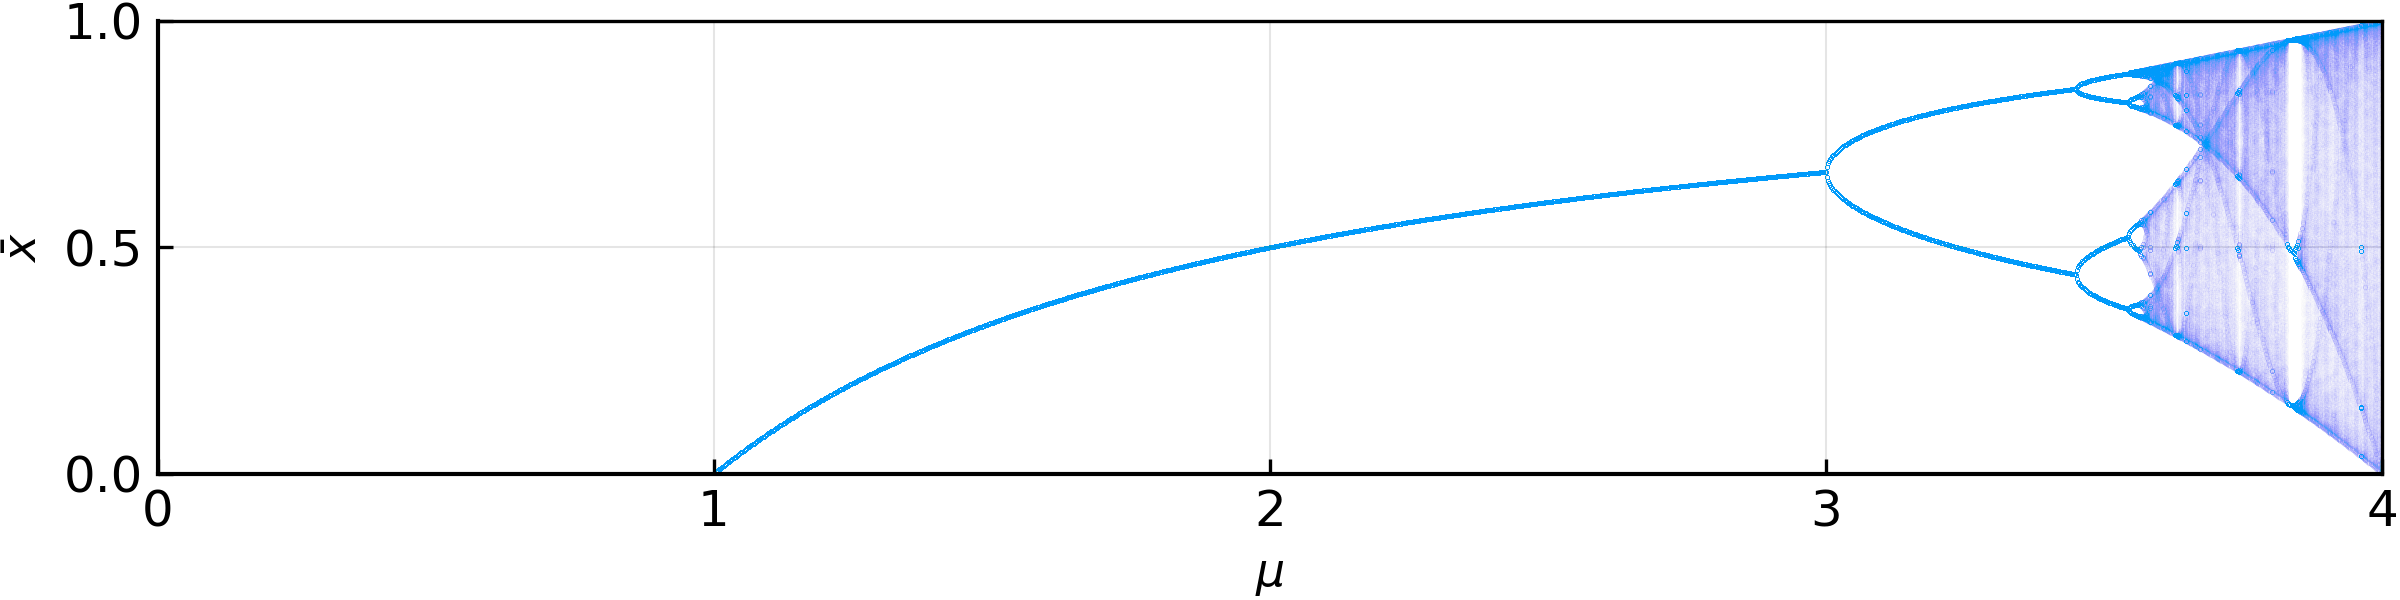
\includegraphics[width=.75\textwidth]{logistic_map_bifurcation_diagram}\\

	Bifurcation diagram of the logistic map $x_{k+1} = \mu x_k \left( 1 - x_k \right)$.
	\vspace{1cm}
\end{frame}

\begin{frame}[t, c]{How are they connected?}{Change of variable}
	\centering
	\begin{block}{\centering \textbf{Exercise}}
		Show that, under an appropriate change of variable $z = f(x)$, the logistic equation can be rewritten as
		$$
		z_{k+1} = z_k^2 + c.
		$$
	\end{block}
	\bigskip
	\underline{\textbf{Hint}}: Assume that $f(x) = \alpha x + \beta$.
	\vspace{1cm}
\end{frame}

\begin{frame}[t, c]{How are they connected?}{Bifurcation diagram ($c$ and $z_0 \in \mathbb{R}$)}
	\centering
	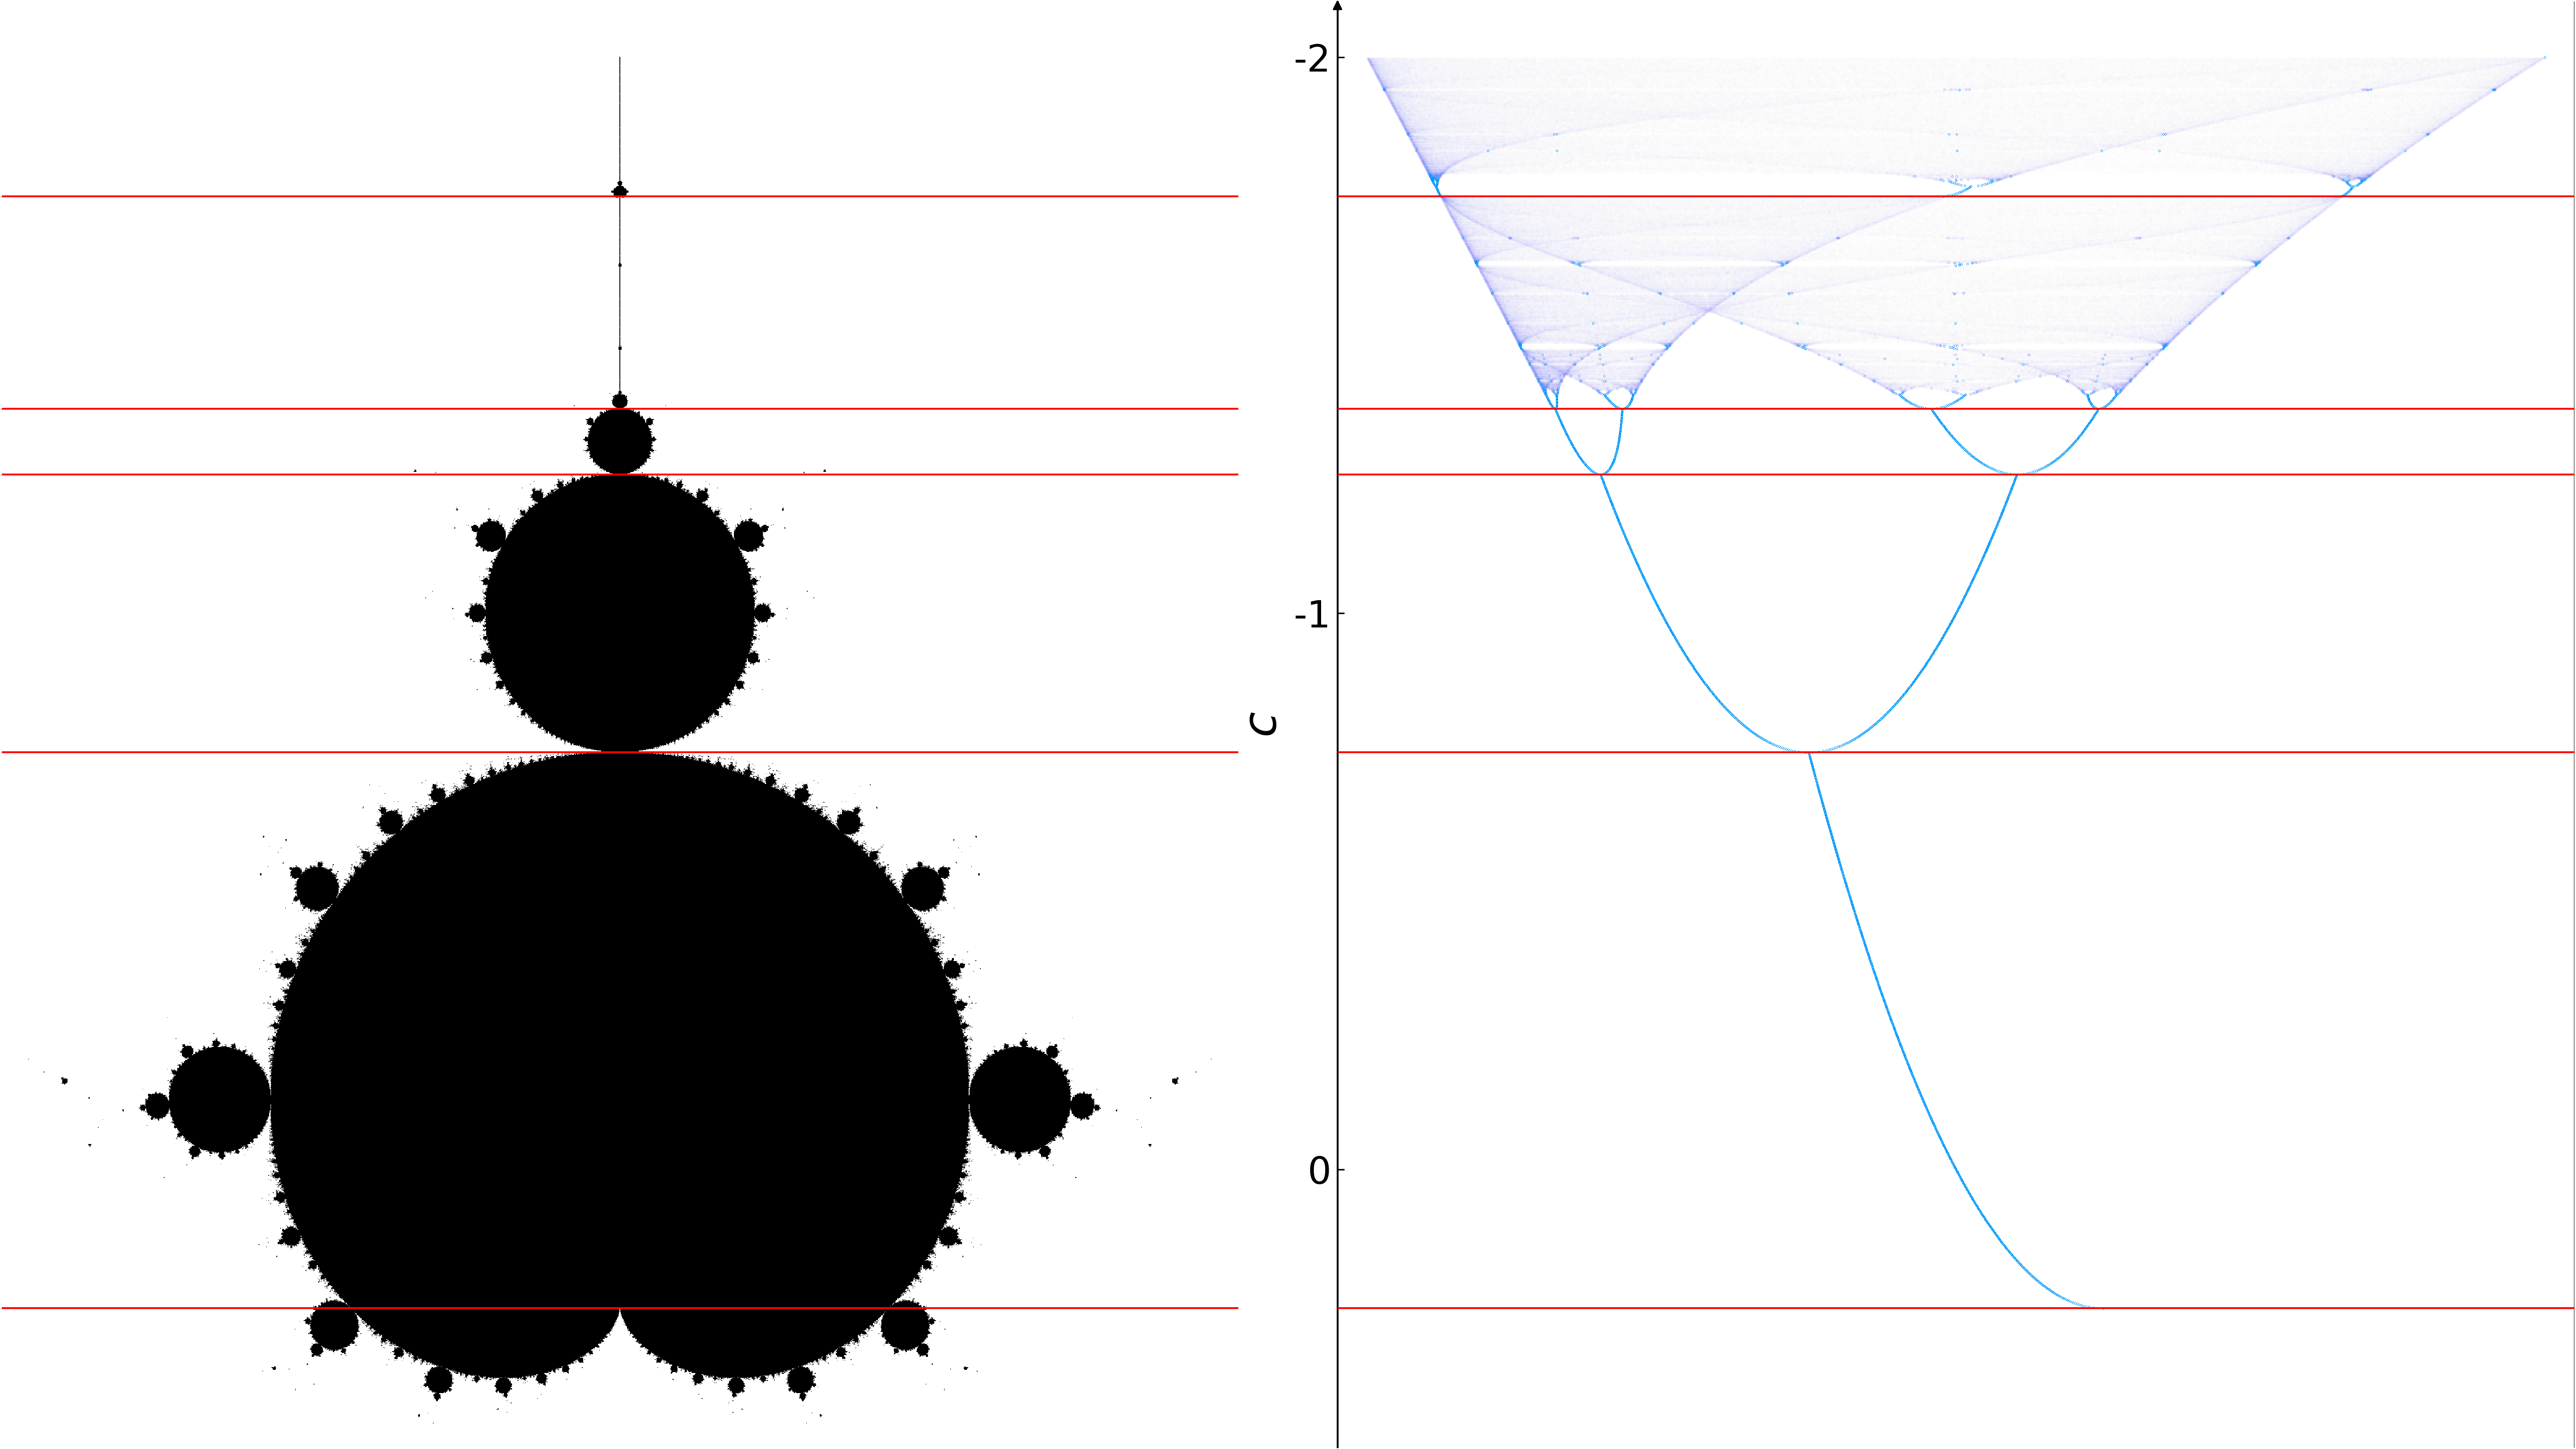
\includegraphics[width=.8\textwidth]{mandelbrot_logistic_bifurcation}
	\vspace{1cm}
\end{frame}

\begin{frame}[t, c]{How are they conected?}{Mandelbrot set and the logistic equation}
	\begin{itemize}
		\item A simple linear change of variable transform the logistic equation into the iteration generating the Mandelbrot set.
		\medskip
		\item The fractal structure of the bifurcation diagram is inherited from that of the Mandelbrot set.
		\begin{itemize}
			\item[$\hookrightarrow$] The Feigenbaum constant also exists within the Mandelbrot set.
			\item[$\hookrightarrow$] Islands of stability correspond to the position of mini-Mandelbrots.
		\end{itemize}
		\medskip
		\item This whole process can be generalized to other unimodel discrete-time dynamical systems, e.g.\ the $\sin$ map.
	\end{itemize}

	\vspace{1cm}
\end{frame}


%-------------------------------------------------------------------------------
%                           CHAOS GAME
%-------------------------------------------------------------------------------


\begin{frame}[t, c]{}
	\centering
	\vspace{1cm}

	{\Large \textbf{Chaos Game}}

	\bigskip

	{\textgre{\textbf{Generating fractal images with simple rules}}}

\end{frame}

\begin{frame}[t, c]{Chaos Game}{Sierpinski Triangle}
	\centering
	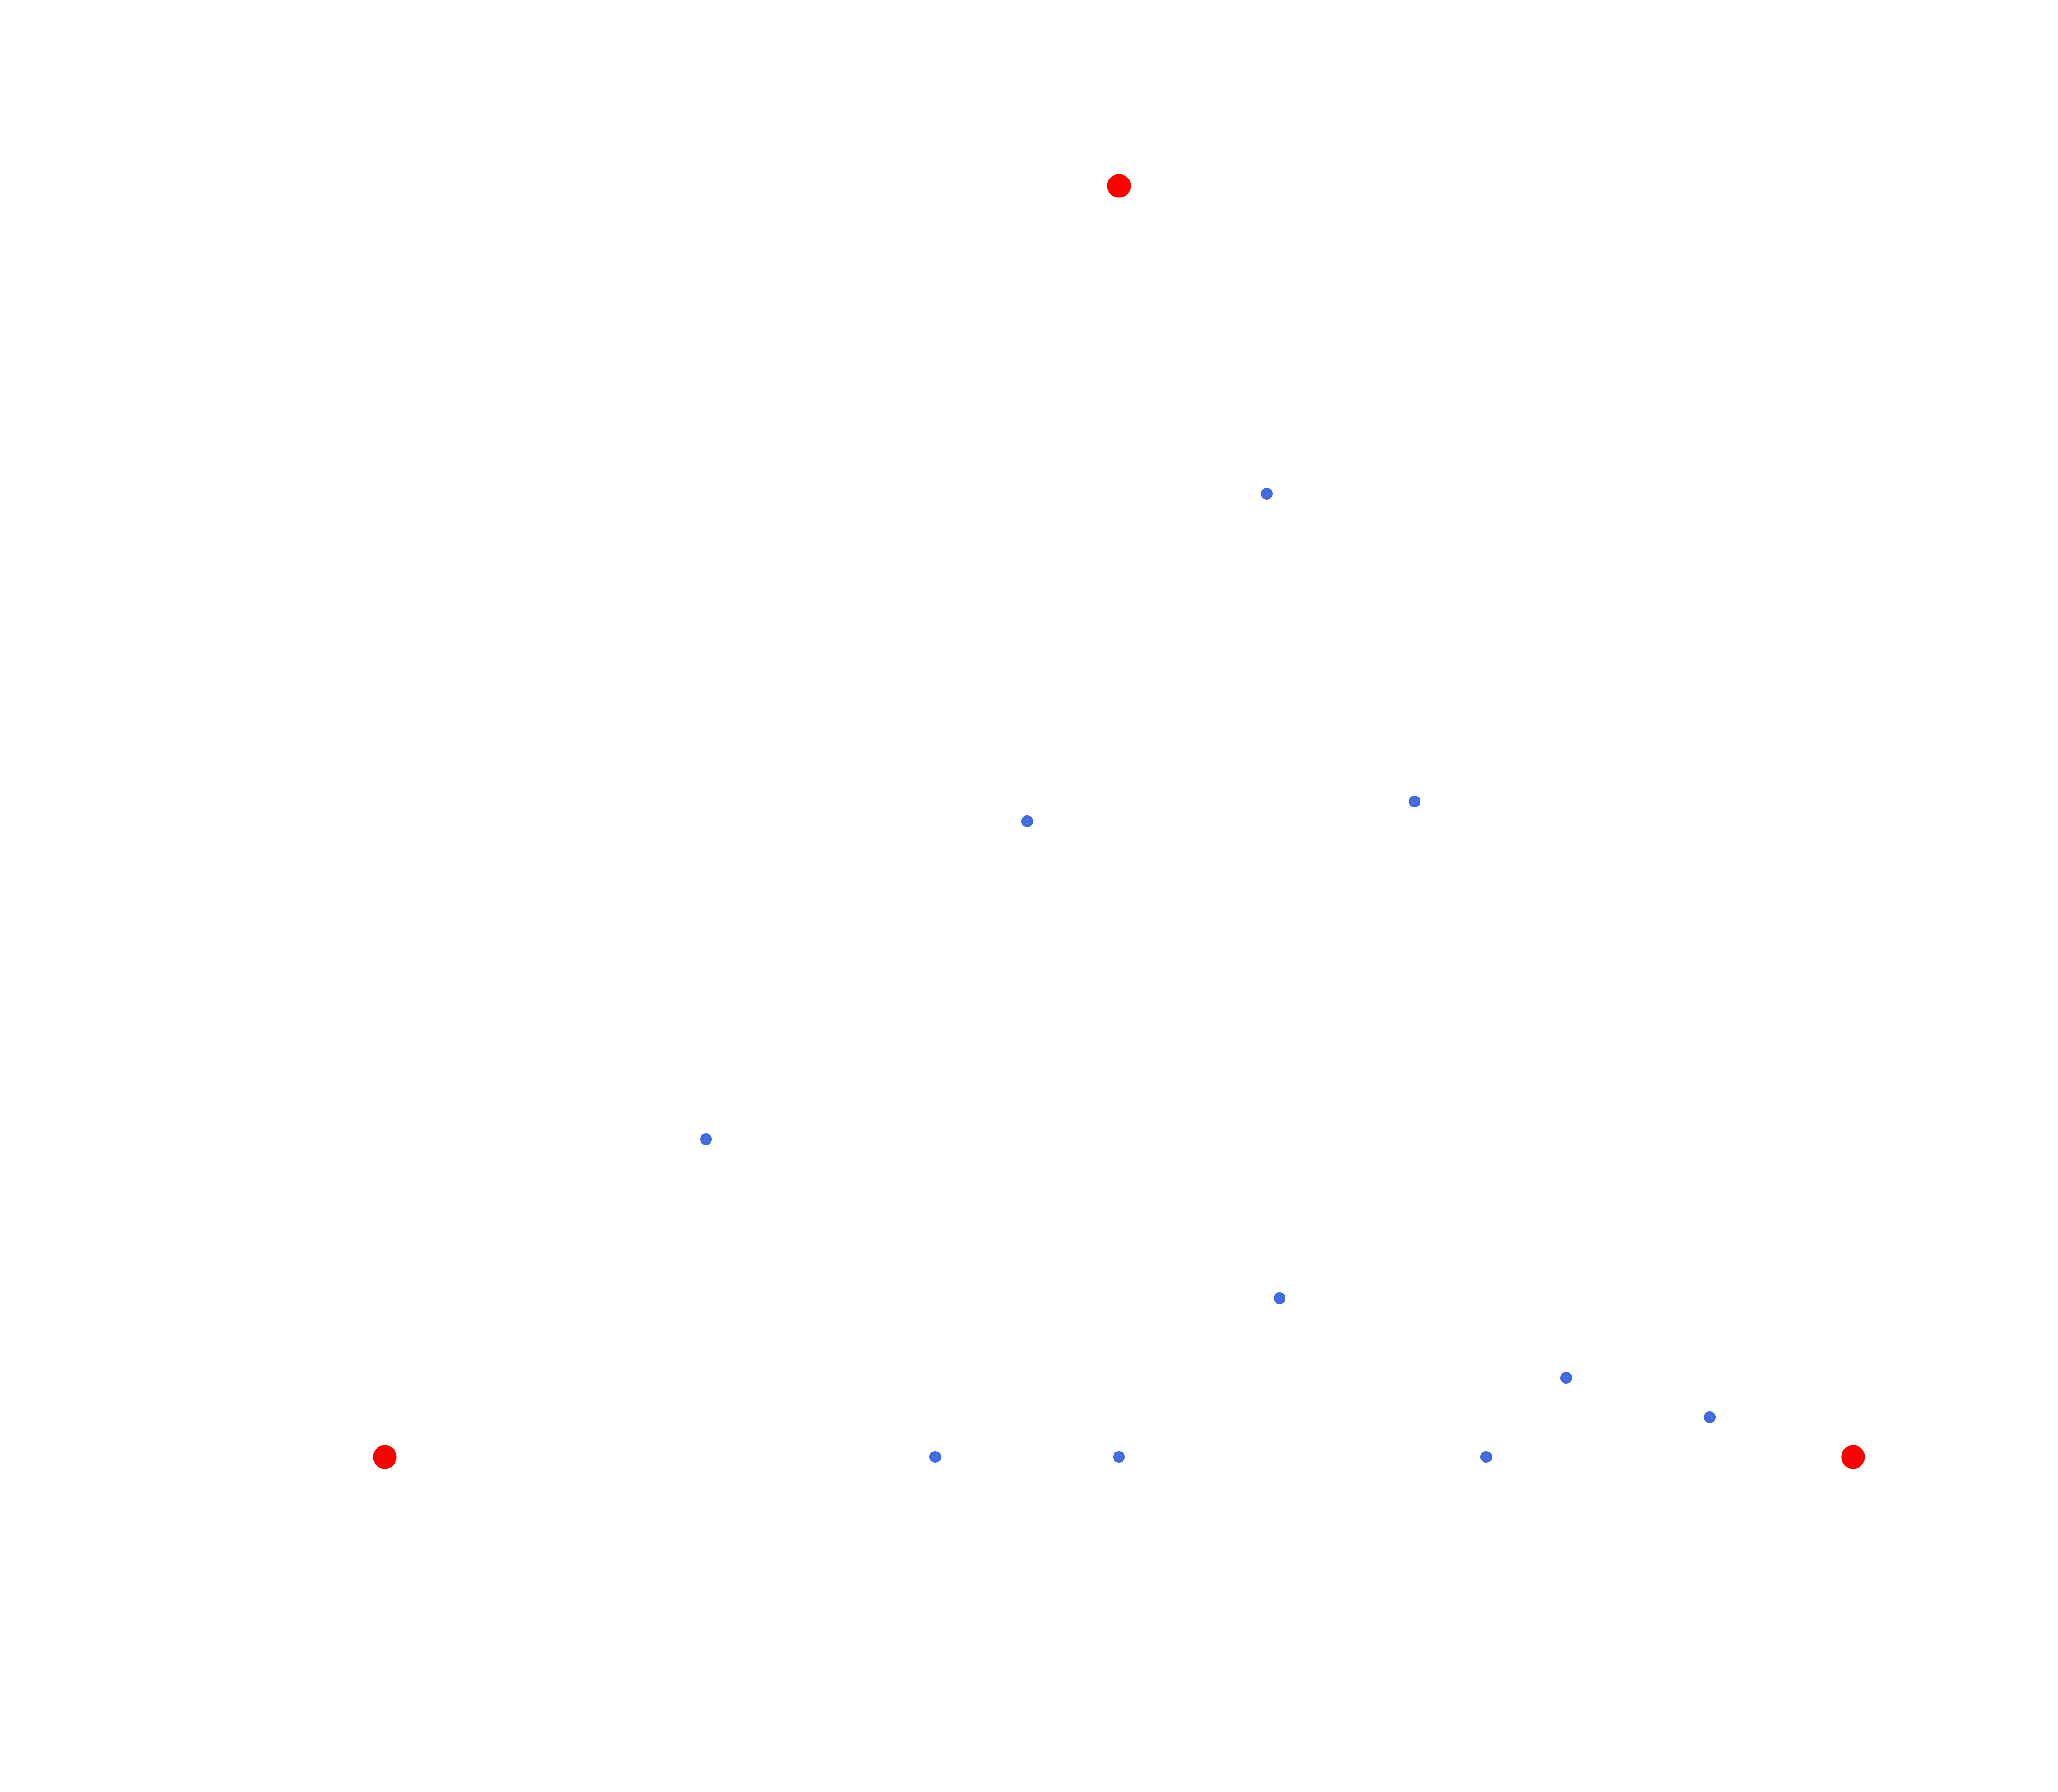
\includegraphics[height=.9\textheight]{sierpinsky_0}
	\vspace{2cm}
\end{frame}

\begin{frame}[t, c]{Chaos Game}{Sierpinski Triangle}
	\centering
	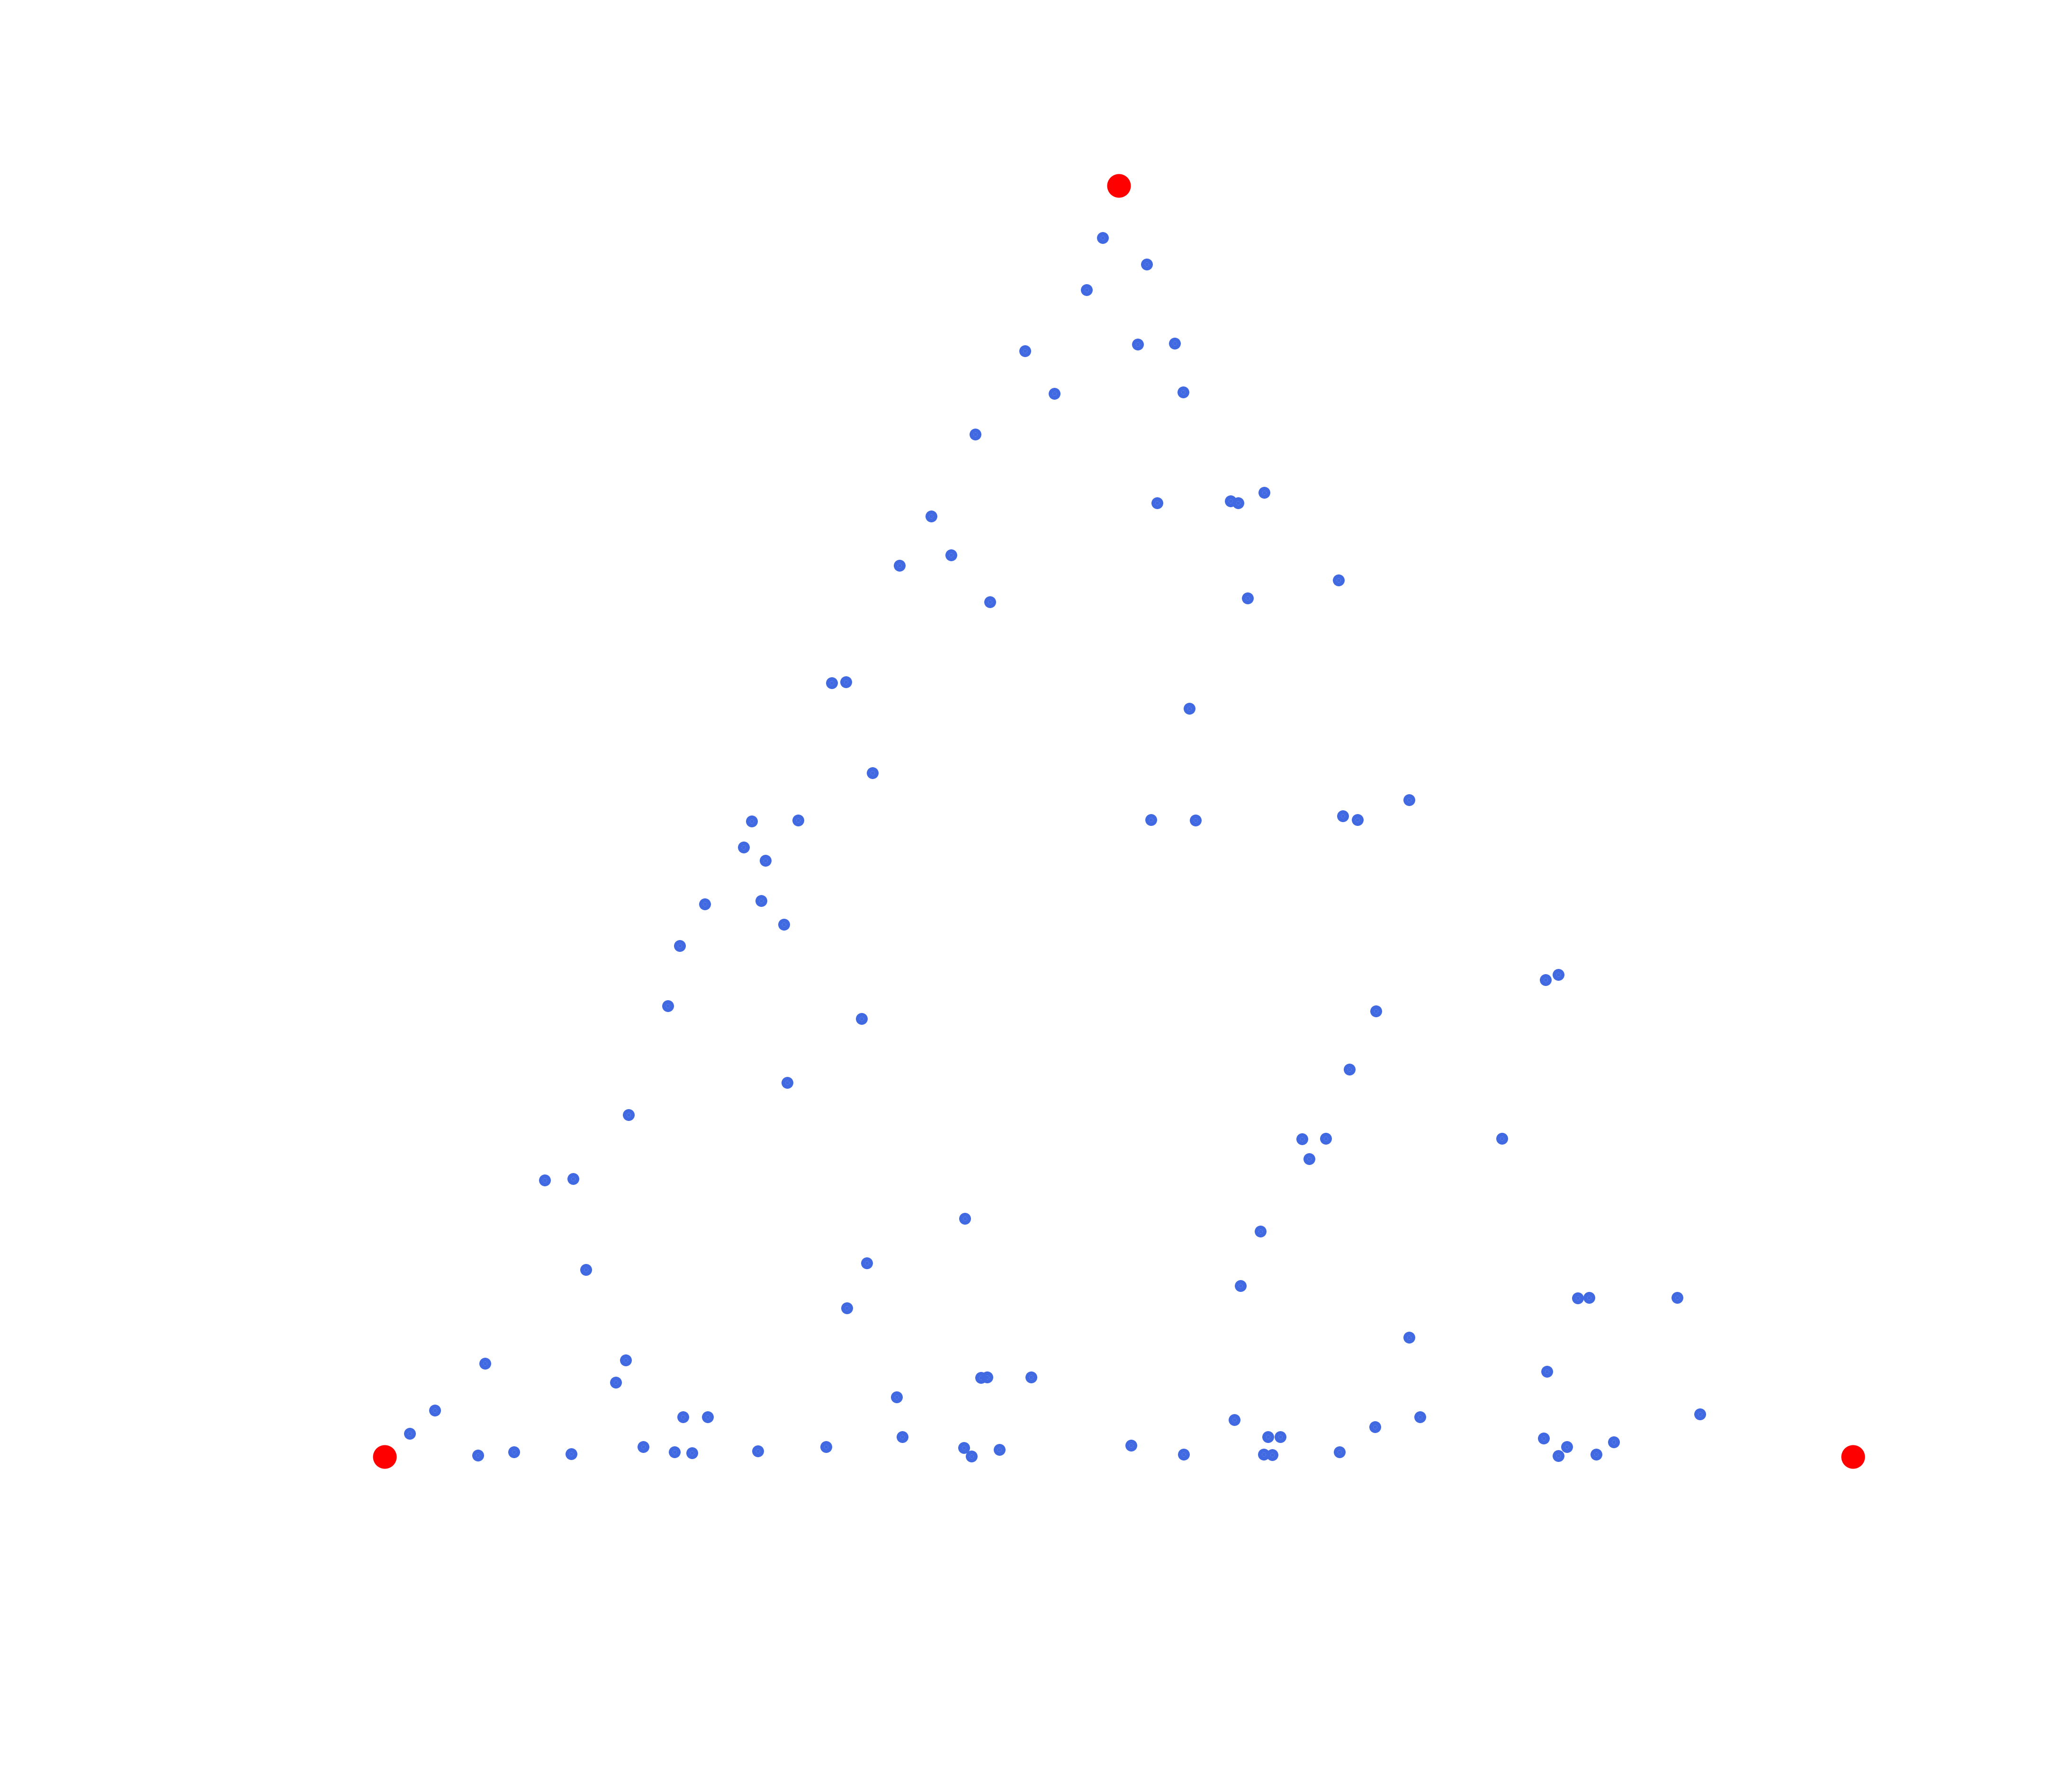
\includegraphics[height=.9\textheight]{sierpinsky_1}
	\vspace{2cm}
\end{frame}

\begin{frame}[t, c]{Chaos Game}{Sierpinski Triangle}
	\centering
	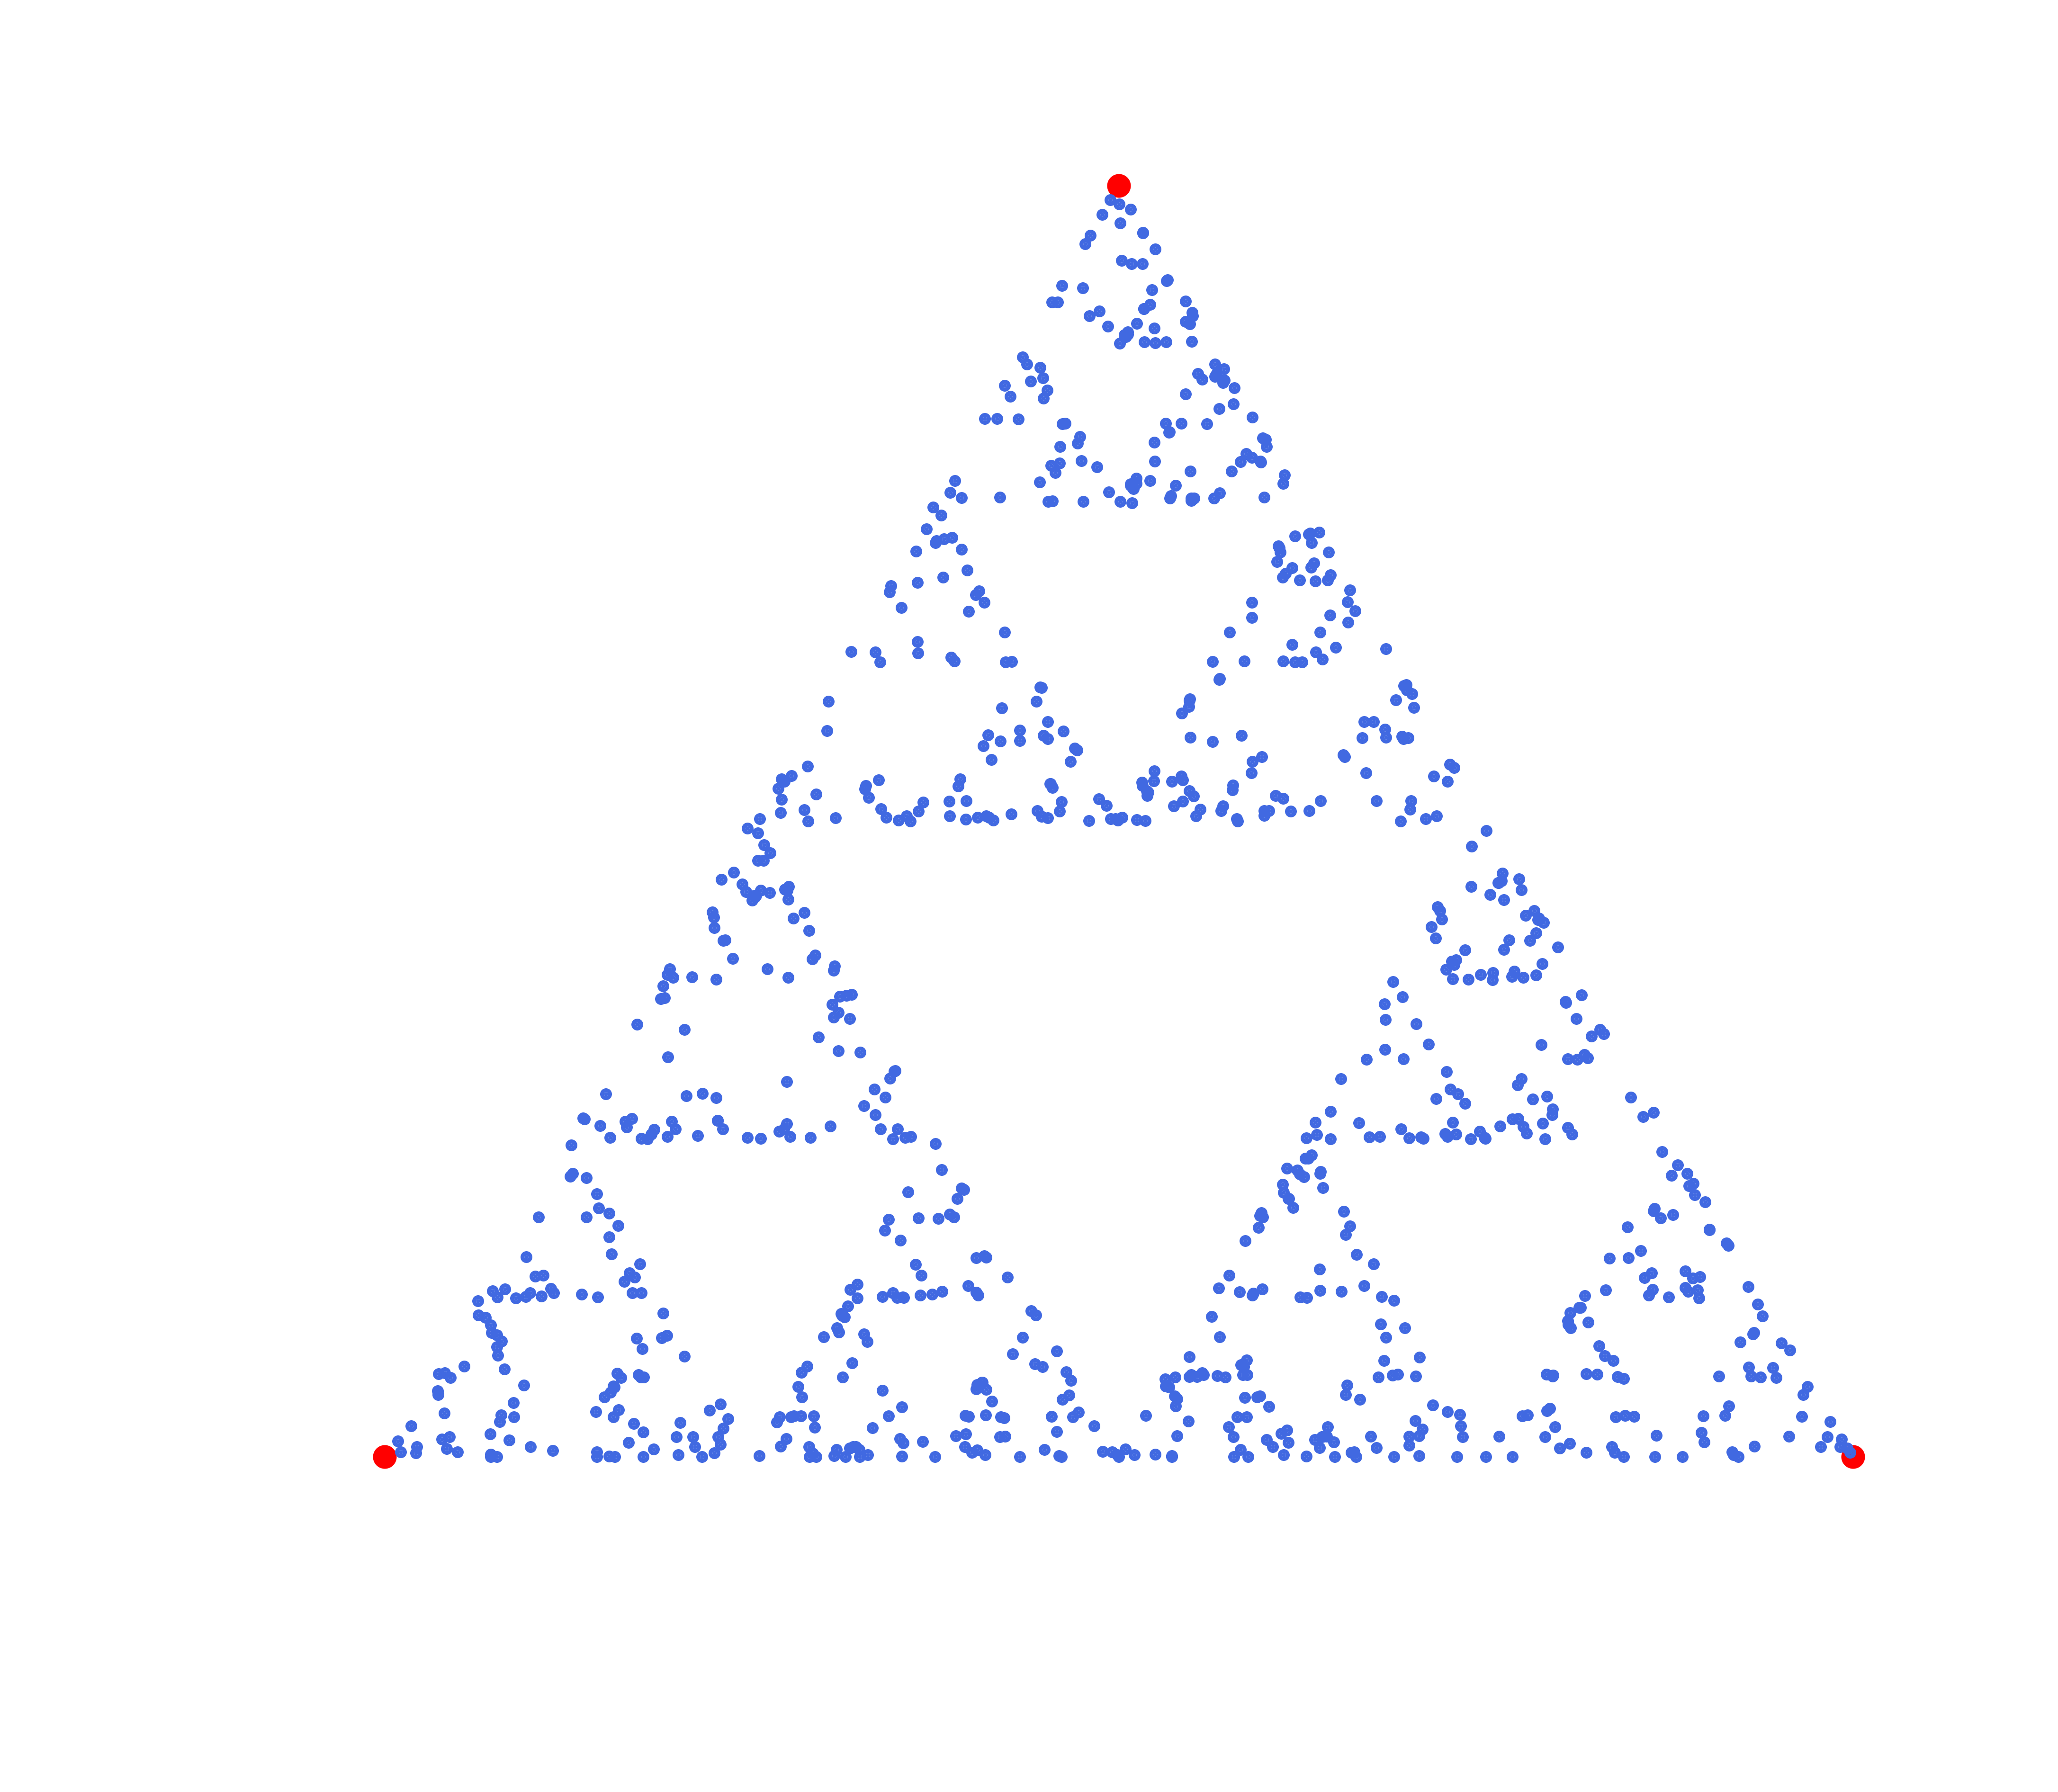
\includegraphics[height=.9\textheight]{sierpinsky_2}
	\vspace{2cm}
\end{frame}

\begin{frame}[t, c]{Chaos Game}{Sierpinski Triangle}
	\centering
	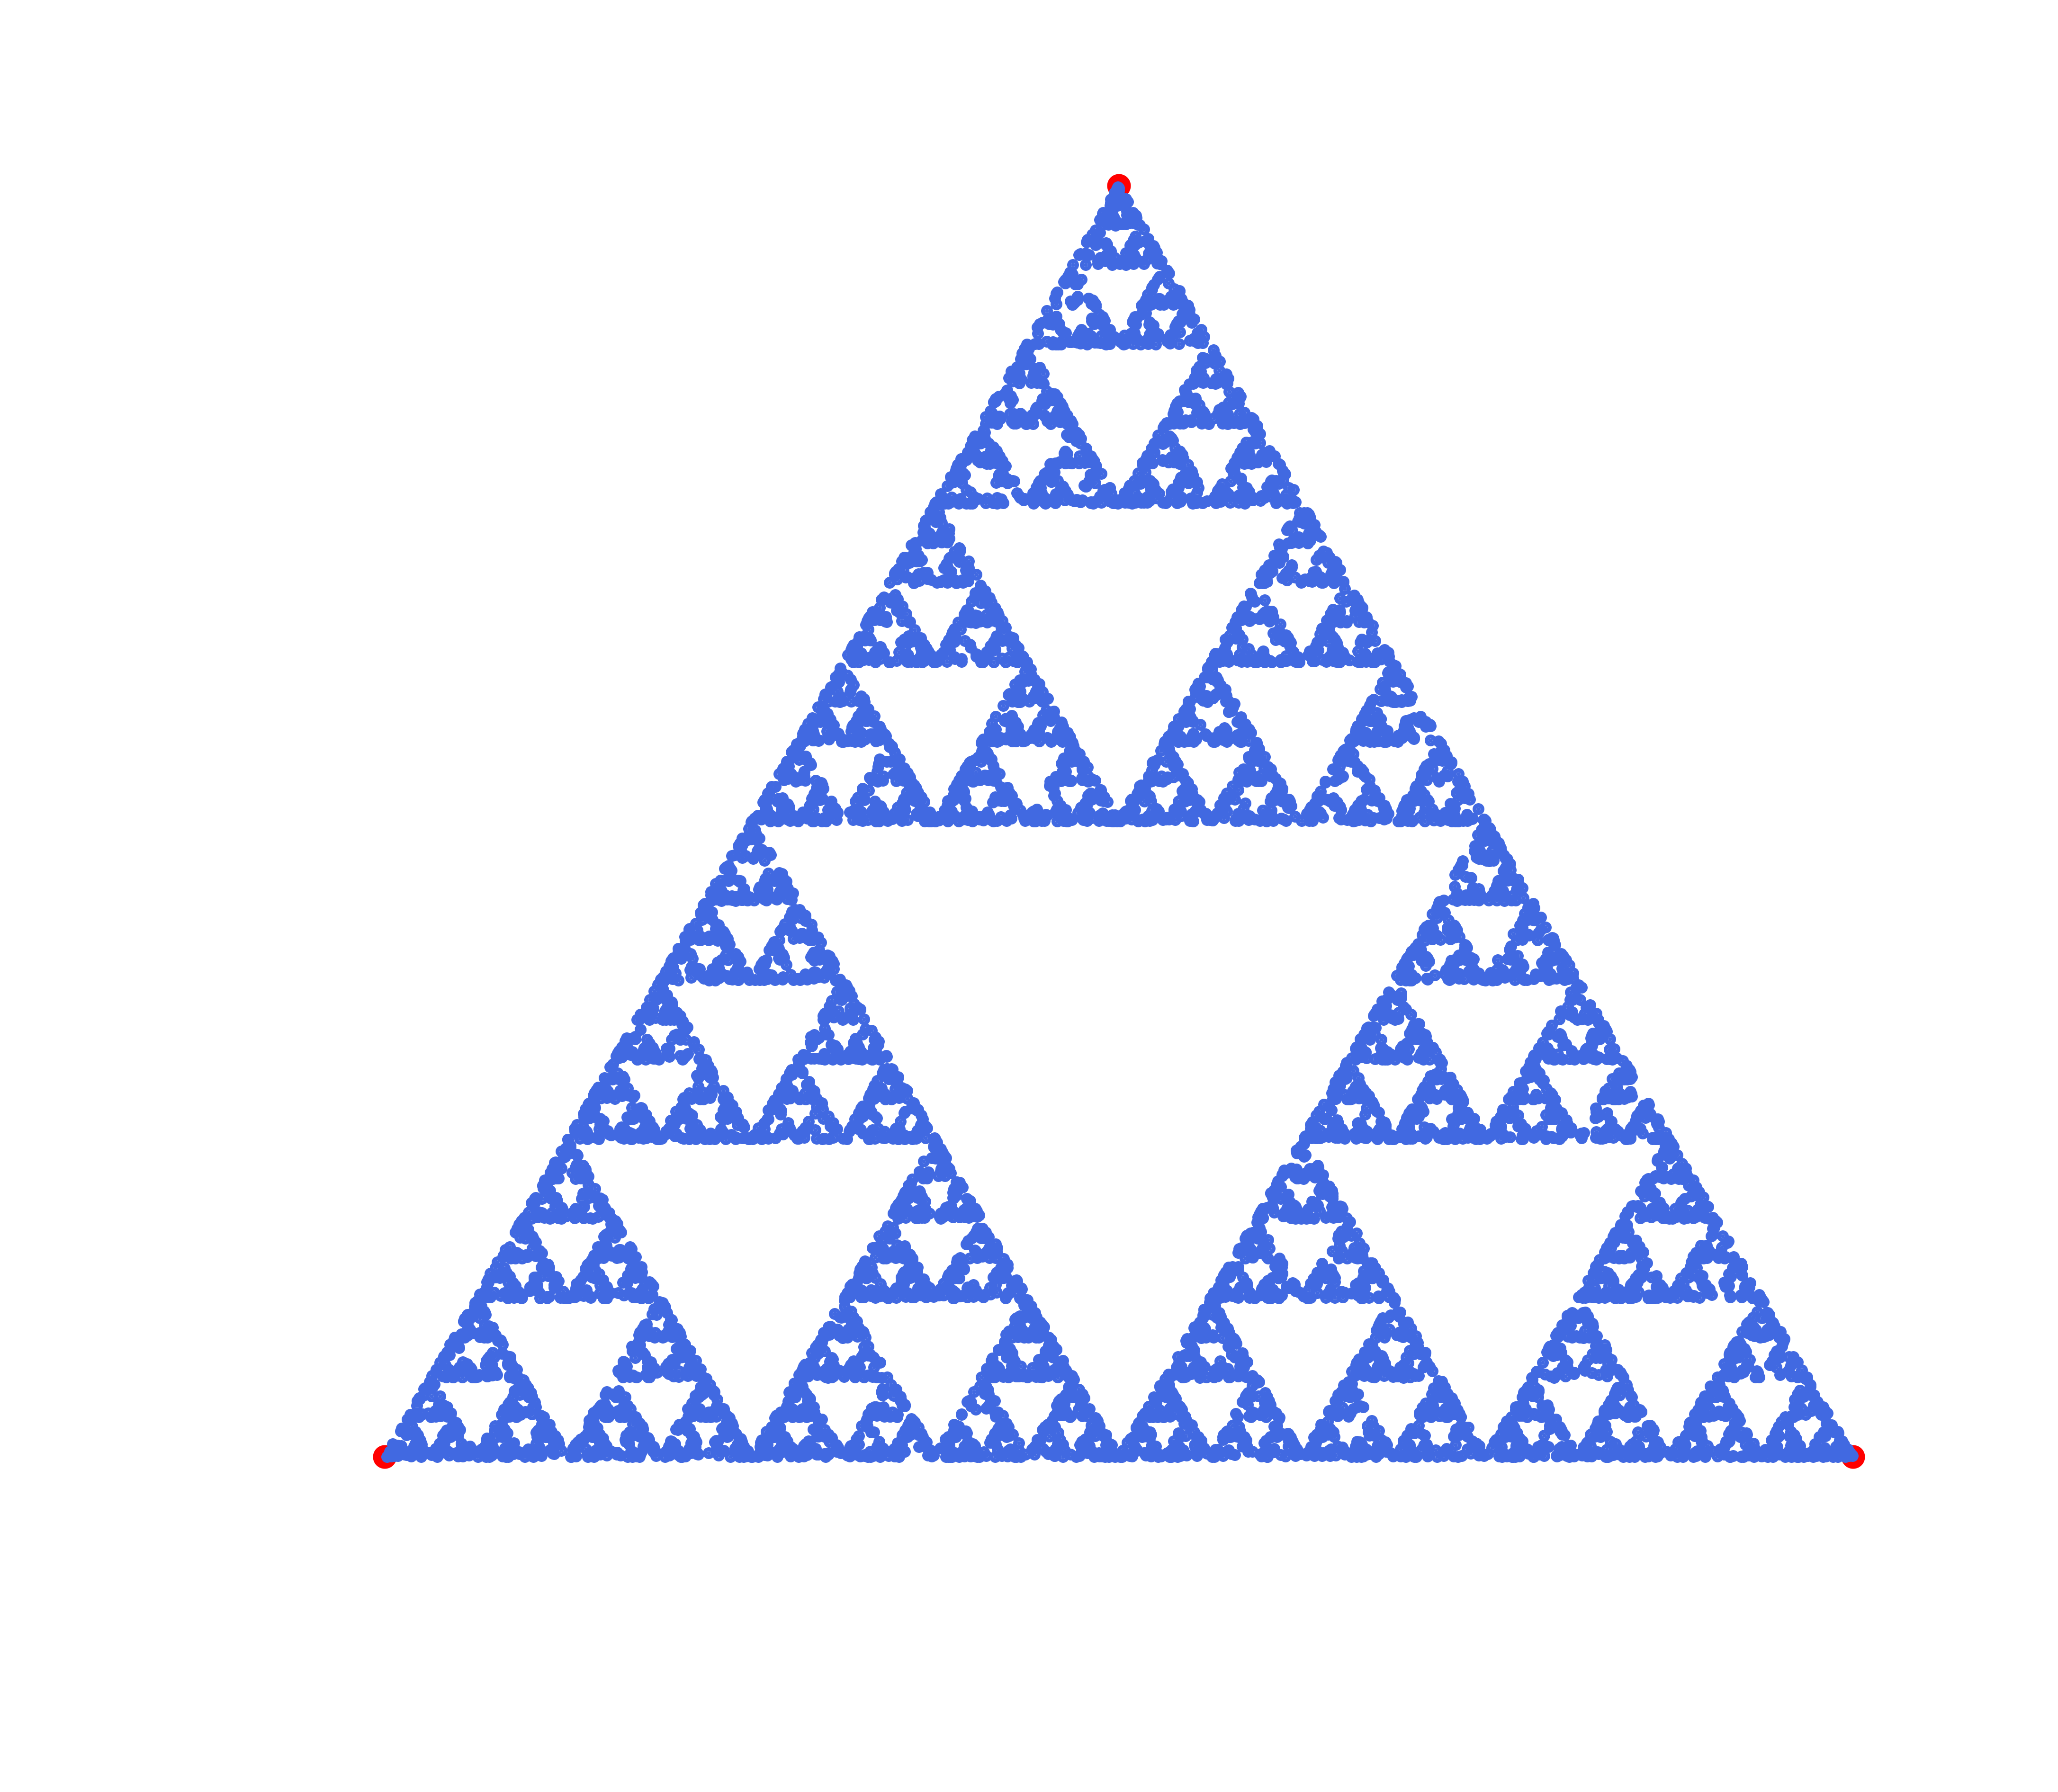
\includegraphics[height=.9\textheight]{sierpinsky_3}
	\vspace{2cm}
\end{frame}

\begin{frame}[t, c]{Chaos Game}{Barnsley Fern}
	\begin{itemize}
		\item Let us consider the following four affine transformations
		\begin{center}
			\begin{tabular}{cccc}
				$f_1(x, y) = \begin{bmatrix} 0 & 0 \\ 0 & 0.16 \end{bmatrix}\begin{bmatrix} x \\ y \end{bmatrix}$ & $f_2(x, y) = \begin{bmatrix} 0.85 & 0.04 \\ -0.04 & 0.85 \end{bmatrix}\begin{bmatrix} x \\ y \end{bmatrix} + \begin{bmatrix} 0 \\ 1.6 \end{bmatrix}$ \\
				\\
				$f_3(x, y) = \begin{bmatrix} 0.2 & -0.26 \\ 0.23 & 0.22 \end{bmatrix}\begin{bmatrix} x \\ y \end{bmatrix} + \begin{bmatrix} 0 \\ 1.6 \end{bmatrix}$ & $f_4(x, y) = \begin{bmatrix} -0.15 & 0.28 \\ 0.26 & 0.24 \end{bmatrix}\begin{bmatrix} x \\ y \end{bmatrix} + \begin{bmatrix} 0 \\ 0.44 \end{bmatrix}$
			\end{tabular}
		\end{center}

		\medskip

		\item Starting from $\bm{x}_0 = (0, 0)$, the point $\bm{x}_{k+1}$ is generated by one of these affine transformation chosen with the following probabilities
		\begin{center}
			\begin{tabular}{cccc}
				$p(f_1) = 0.01$ & $p(f_2) = 0.85$ & $p(f_3) = 0.07$ & $p(f_4) = 0.07$
			\end{tabular}
		\end{center}
	\end{itemize}
\end{frame}

\begin{frame}[t, c]{Chaos Game}{Barnsley Fern}
	\centering
	
\includegraphics[width=.8\textwidth]{Barnsley_fern_0}
	\vspace{1cm}
\end{frame}

\begin{frame}[t, c]{Chaos Game}{Barnsley Fern}
	\centering
	
\includegraphics[width=.8\textwidth]{Barnsley_fern_1}
	\vspace{1cm}
\end{frame}

\begin{frame}[t, c]{Chaos Game}{Barnsley Fern}
	\centering
	
\includegraphics[width=.8\textwidth]{Barnsley_fern_2}
	\vspace{1cm}
\end{frame}

\begin{frame}[t, c]{Chaos Game}{Barnsley Fern}
	\centering
	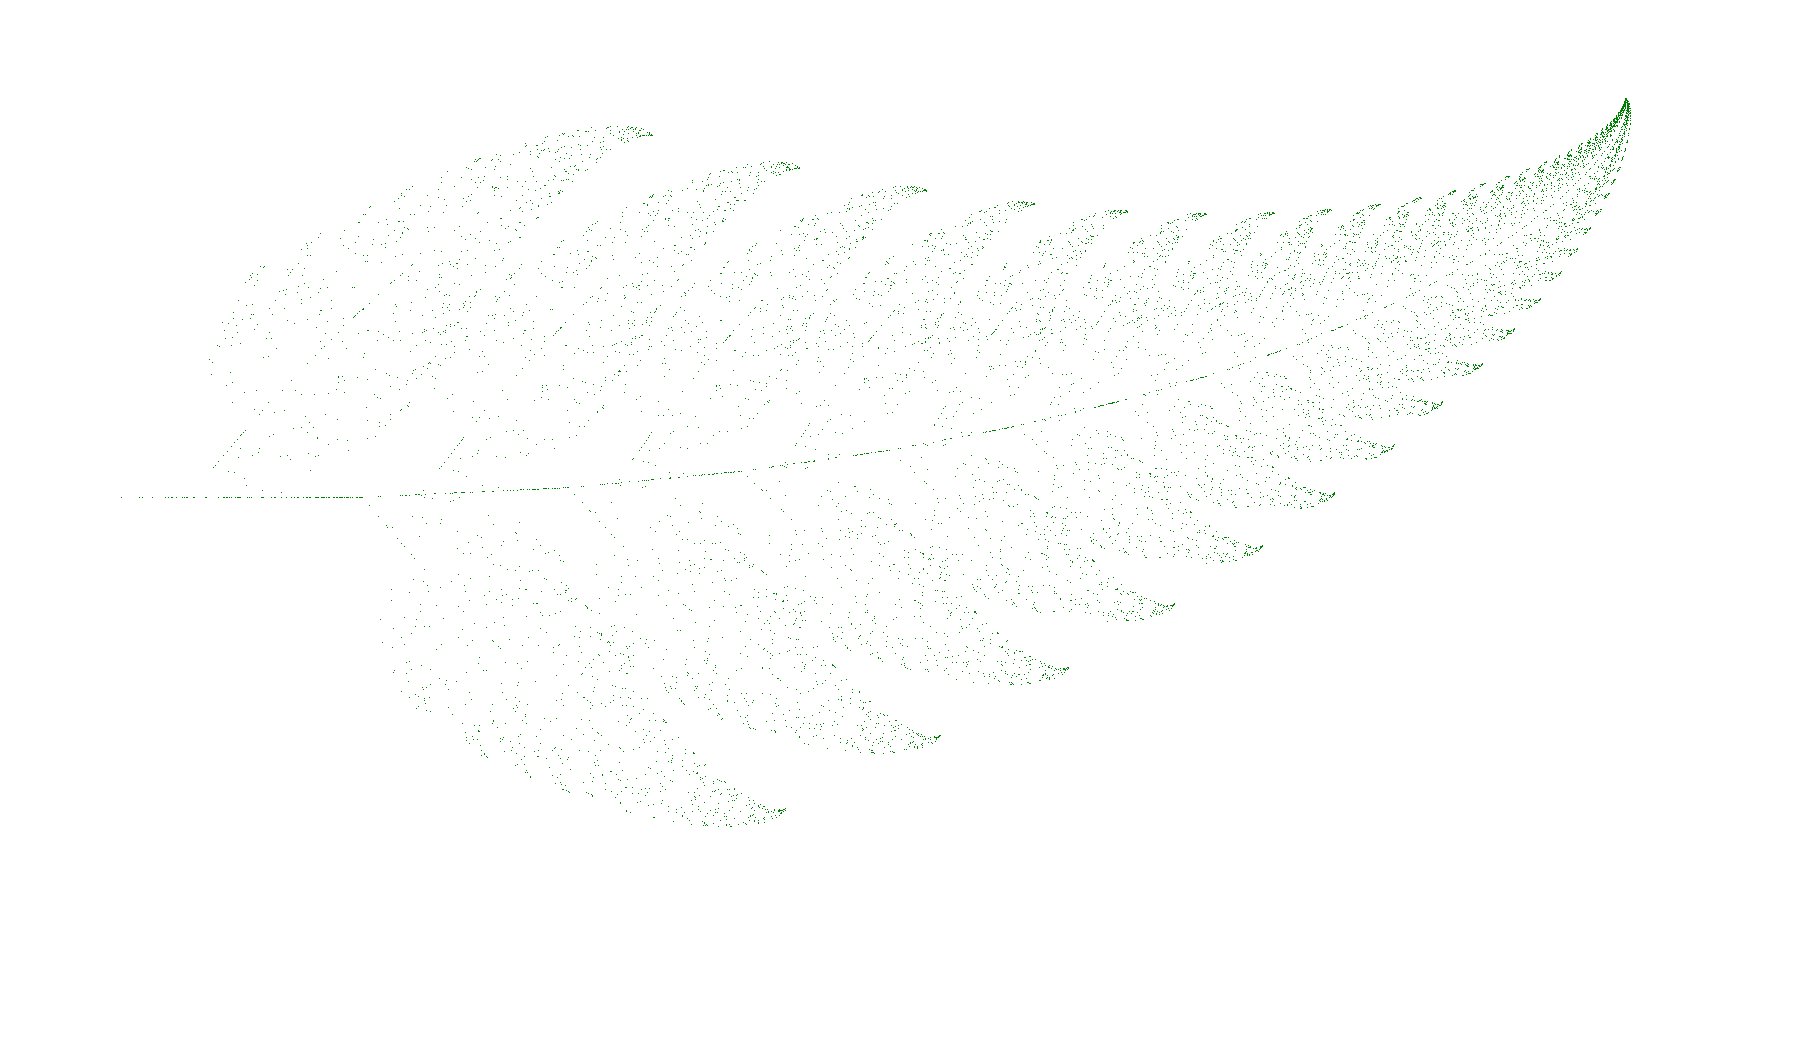
\includegraphics[width=.8\textwidth]{Barnsley_fern_3}
	\vspace{1cm}
\end{frame}

\begin{frame}[t, c]{Chaos Game}{Barnsley Fern}
	\centering
	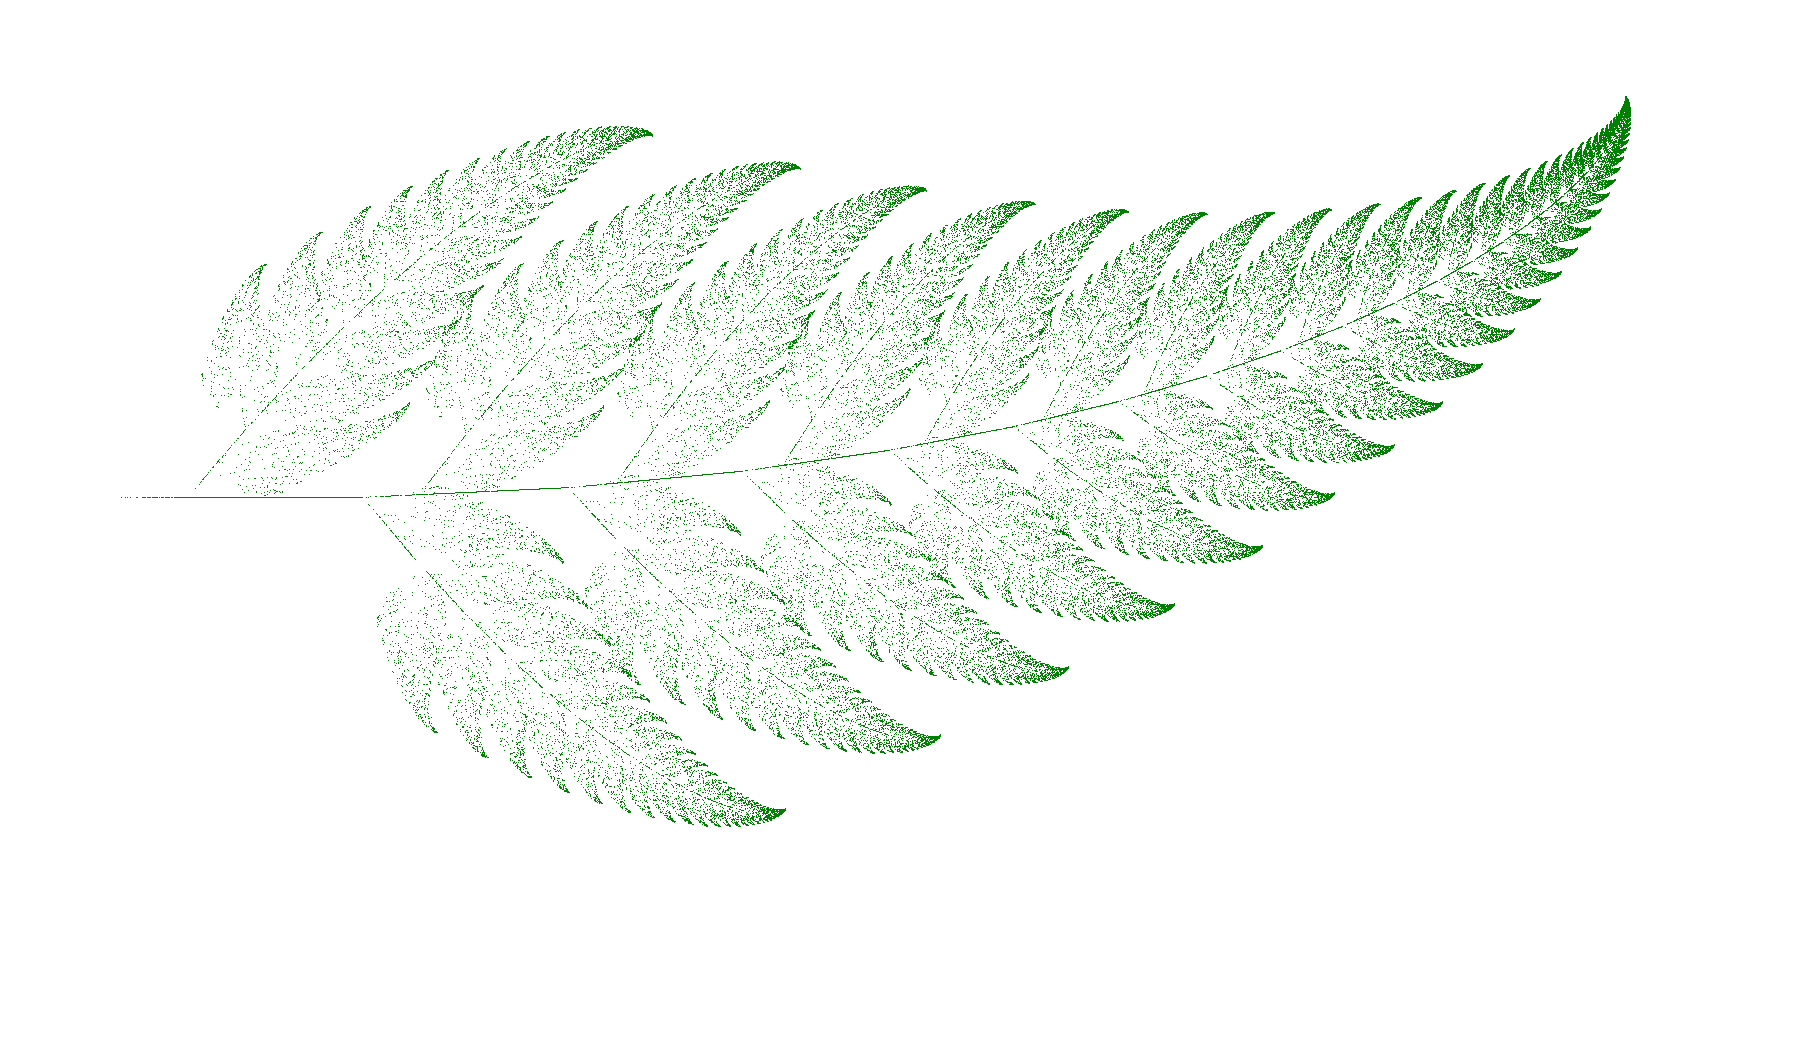
\includegraphics[width=.8\textwidth]{Barnsley_fern_4}
	\vspace{1cm}
\end{frame}

\begin{frame}[t, c]{Chaos Game}{Barnsley Fern}
	\centering
	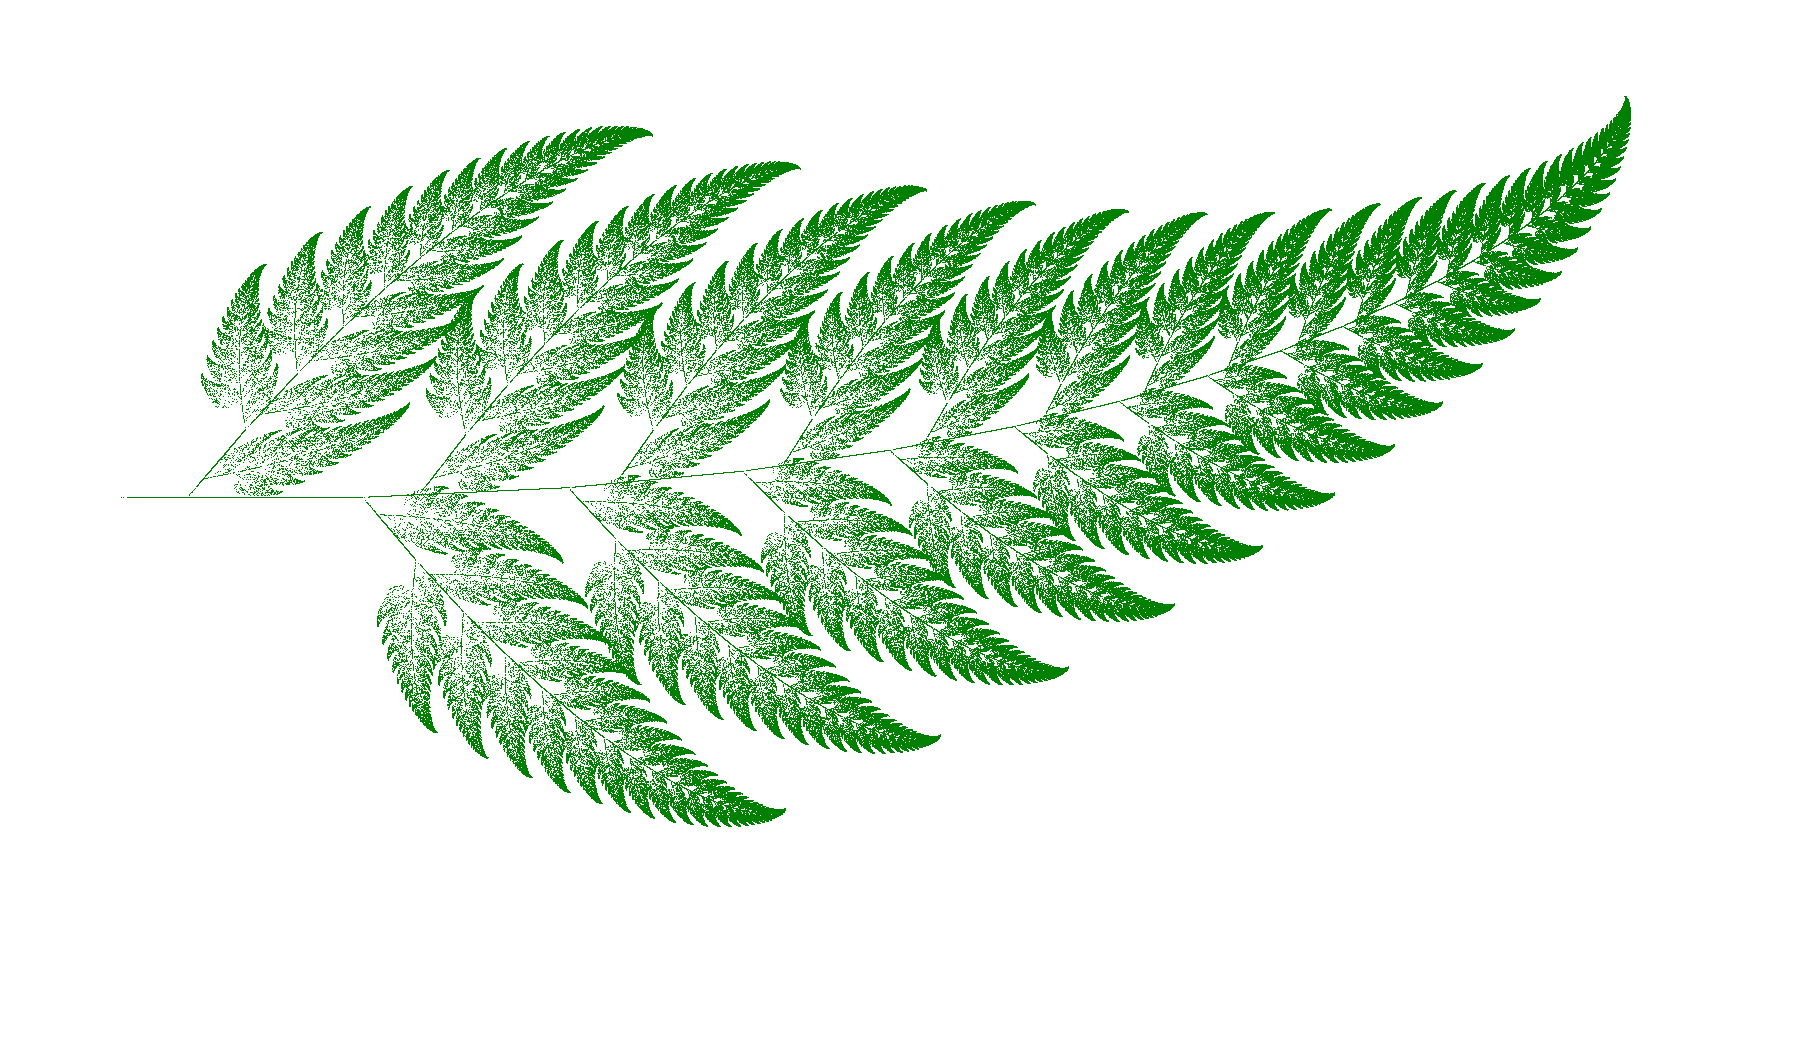
\includegraphics[width=.8\textwidth]{Barnsley_fern_5}
	\vspace{1cm}
\end{frame}

\begin{frame}[t, c]{Chaos Game}{Barnsley Fern}
	\centering
	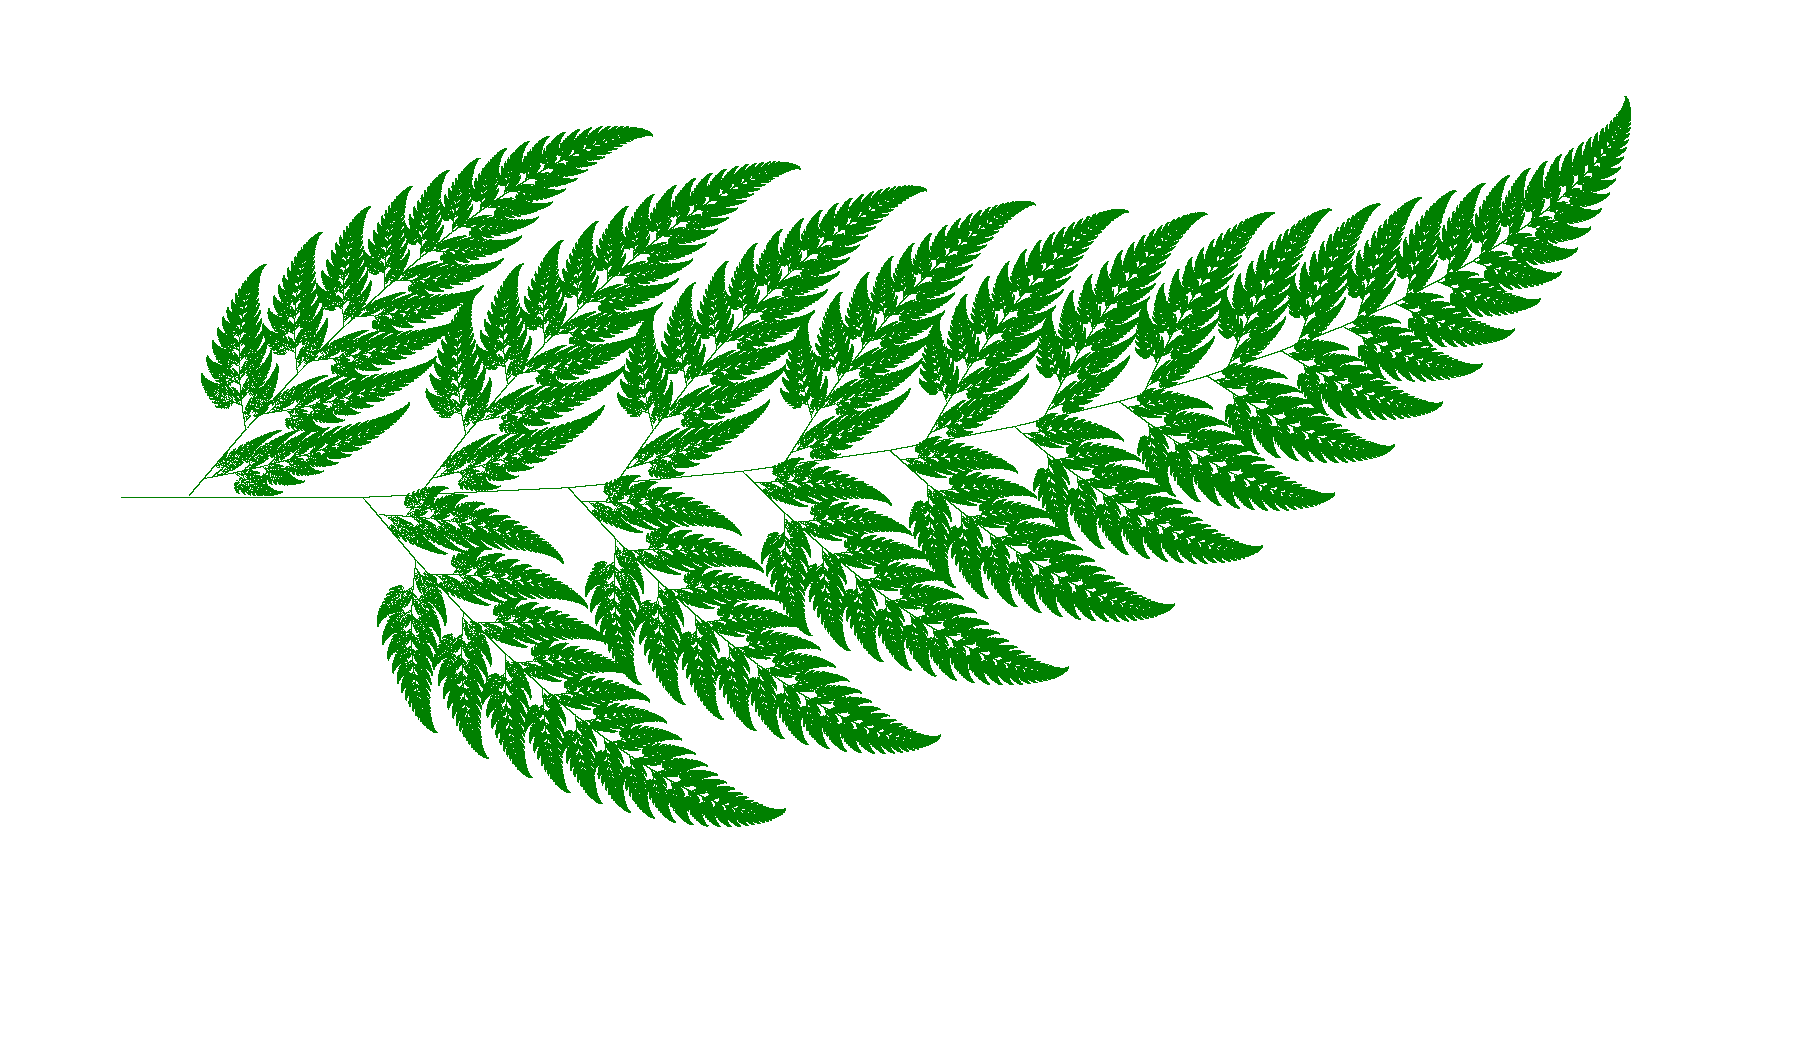
\includegraphics[width=.8\textwidth]{Barnsley_fern_6}
	\vspace{1cm}
\end{frame}



\begin{frame}[t, c]{Chaos Game}{Mapple leaf}
	\begin{itemize}
		\item Let us consider the following four affine transformations
		\begin{center}
			\begin{tabular}{cccc}
				$f_1(x, y) = \begin{bmatrix} 0.14 & 0.01 \\ 0 & 0.51 \end{bmatrix}\begin{bmatrix} x \\ y \end{bmatrix} + \begin{bmatrix} -0.08 \\ -1.31 \end{bmatrix}$ & $f_2(x, y) = \begin{bmatrix} 0.43 & 0.52 \\ -0.45 & 0.5 \end{bmatrix}\begin{bmatrix} x \\ y \end{bmatrix} + \begin{bmatrix} 1.49 \\ -0.75 \end{bmatrix}$ \\
				\\
				$f_3(x, y) = \begin{bmatrix} 0.45 & -0.49 \\ 0.47 & 0.47 \end{bmatrix}\begin{bmatrix} x \\ y \end{bmatrix} + \begin{bmatrix} -1.62 \\ -0.74 \end{bmatrix}$ & $f_4(x, y) = \begin{bmatrix} 0.49 & 0 \\ 0 & 0.51 \end{bmatrix}\begin{bmatrix} x \\ y \end{bmatrix} + \begin{bmatrix} 0.02 \\ 1.62 \end{bmatrix}$
			\end{tabular}
		\end{center}

		\medskip

		\item Starting from $\bm{x}_0 = (0, 0)$, the point $\bm{x}_{k+1}$ is generated by one of these affine transformation chosen with the following probabilities
		\begin{center}
			\begin{tabular}{cccc}
				$p(f_1) = 0.1$ & $p(f_2) = 0.35$ & $p(f_3) = 0.35$ & $p(f_4) = 0.2$
			\end{tabular}
		\end{center}
	\end{itemize}
\end{frame}

\begin{frame}[t, c]{Chaos Game}{Mapple leaf}
	\centering
	
\includegraphics[height=.8\textheight]{Mapple_leaf_0}
	\vspace{1cm}
\end{frame}

\begin{frame}[t, c]{Chaos Game}{Mapple leaf}
	\centering
	
\includegraphics[height=.8\textheight]{Mapple_leaf_1}
	\vspace{1cm}
\end{frame}

\begin{frame}[t, c]{Chaos Game}{Mapple leaf}
	\centering
	
\includegraphics[height=.8\textheight]{Mapple_leaf_2}
	\vspace{1cm}
\end{frame}

\begin{frame}[t, c]{Chaos Game}{Mapple leaf}
	\centering
	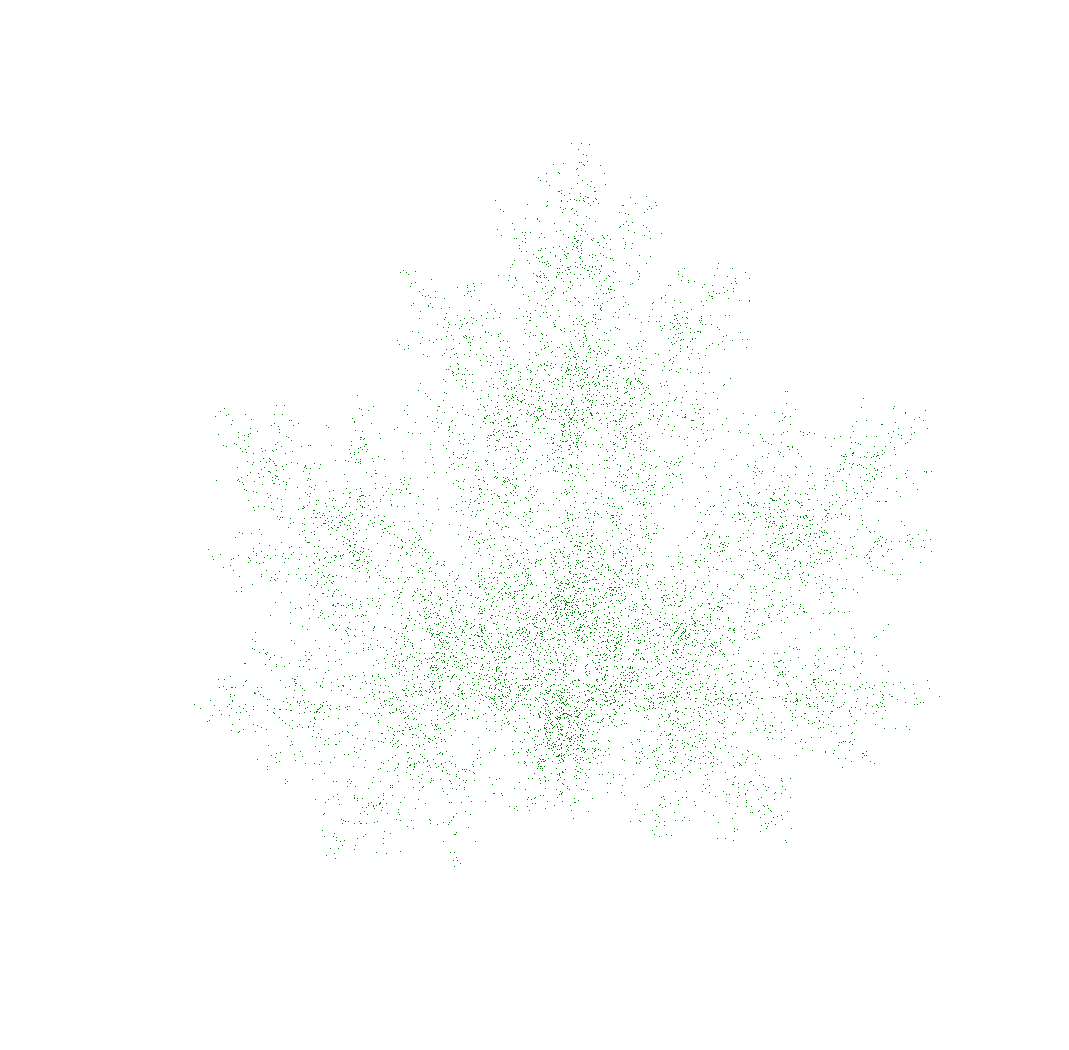
\includegraphics[height=.8\textheight]{Mapple_leaf_3}
	\vspace{1cm}
\end{frame}

\begin{frame}[t, c]{Chaos Game}{Mapple leaf}
	\centering
	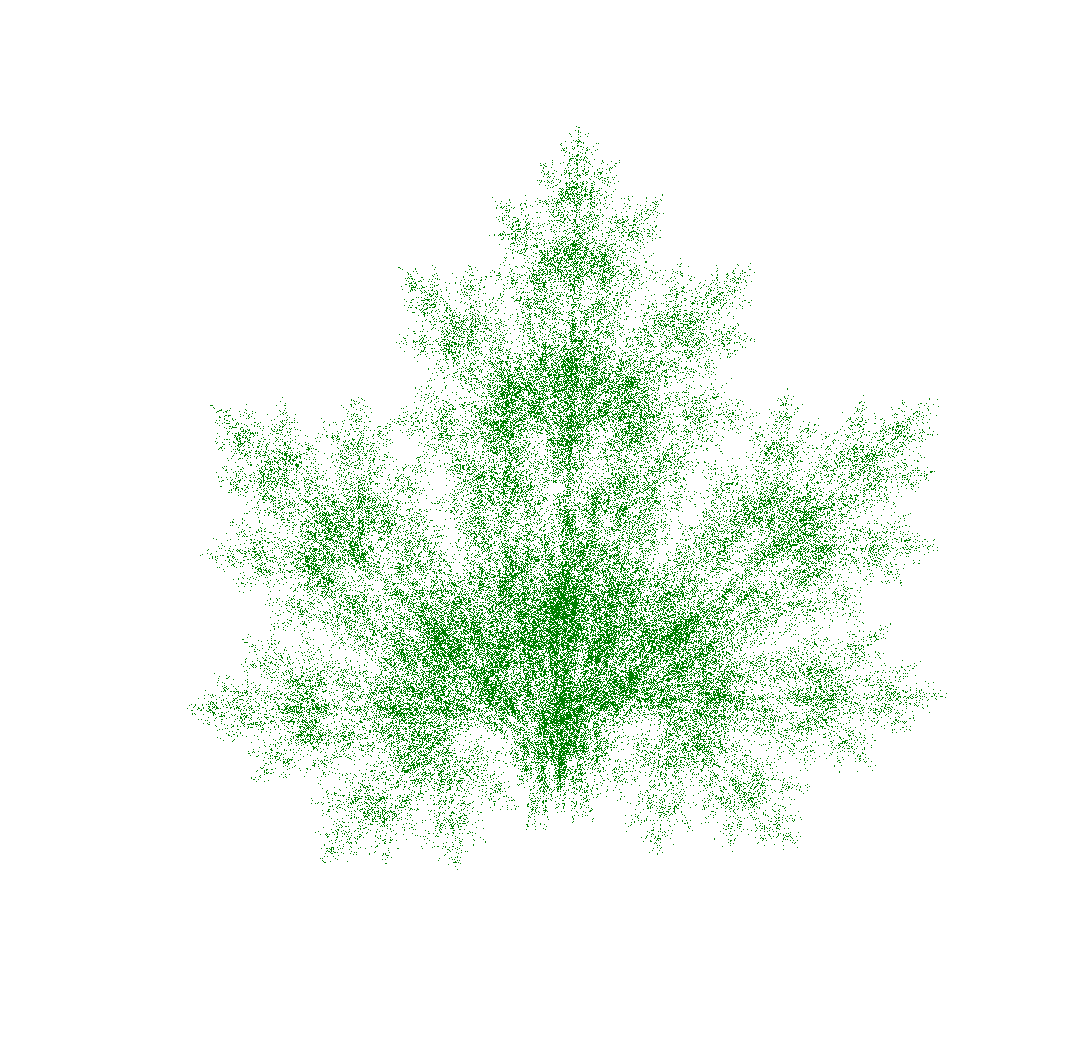
\includegraphics[height=.8\textheight]{Mapple_leaf_4}
	\vspace{1cm}
\end{frame}

\begin{frame}[t, c]{Chaos Game}{Mapple leaf}
	\centering
	\includegraphics[height=.8\textheight]{Mapple_leaf_5}
	\vspace{1cm}
\end{frame}

\begin{frame}[t, c]{Chaos Game}{Mapple leaf}
	\centering
	\includegraphics[height=.8\textheight]{Mapple_leaf_6}
	\vspace{1cm}
\end{frame}


%-------------------------------------------------------------------------------
%                           PLOT IMAGES
%-------------------------------------------------------------------------------


\begin{frame}[t, c]{}
	\centering
	\vspace{1cm}

	{\Large \textbf{How to plot these images?}}

	\bigskip

	{\textgre{\textbf{Computer time}}}

\end{frame}


\end{document}
